\documentclass[twoside,11pt]{report}
\usepackage{tabularx} % extra features for tabular environment
\usepackage{amsmath}  % improve math presentation
\usepackage{graphicx, subcaption} % takes care of graphic including machinery
\usepackage{fancyhdr}
\pagestyle{fancy}
\setlength{\headheight}{13.59999pt}
\usepackage[top=2.5cm, bottom=2.5cm, left=4.0cm, right=2.5cm]{geometry}
% \usepackage[margin=1in,letterpaper]{geometry} % decreases margins
\usepackage{xspace}
\usepackage{ANA-FTAG-2020-08-PAPER-defs}
\usepackage[style=numeric, sorting=none]{biblatex}
\addbibresource{ANA-FTAG-2020-08-PAPER.bib}
\addbibresource{Detector.bib}
\addbibresource{reconstruction.bib}
\addbibresource{bib/ATLAS.bib}
\addbibresource{bib/ATLAS-useful.bib}
\addbibresource{bib/PubNotes.bib}
\addbibresource{bib/ConfNotes.bib}
\addbibresource{bib/ATLAS-SUSY.bib}

\usepackage[final]{hyperref} % adds hyper links inside the generated pdf file
\usepackage[T1]{fontenc}
\usepackage{setspace}
\usepackage{float}
\usepackage{makeidx}
\usepackage{titlesec}
\usepackage{multirow}
\usepackage{titling}
\newcommand\bjetineq{\mathop{\mbox{$b$ $\rm{jet}$}}}
\newcommand\bjetunder{\mathop{\footnotesize{\mbox{$b$ $\rm{jet}$}}}\normalsize}
\newcommand\cjetineq{\mathop{\mbox{$c$ $\rm{jet}$}}}
\newcommand\cjetunder{\mathop{\footnotesize{\mbox{$c$ $\rm{jet}$}}}\normalsize}
\setcounter{secnumdepth}{4}
\newcommand{\specialcell}[2][c]{%
  \begin{tabular}[#1]{@{}c@{}}#2\end{tabular}}
\newcommand{\changefont}{\fontsize{9}{11}\selectfont}
\titleformat{\paragraph}
{\normalfont\normalsize\bfseries}{\theparagraph}{1em}{}
\titlespacing*{\paragraph}
{0pt}{3.25ex plus 1ex minus .2ex}{1.5ex plus .2ex}
\restylefloat*{figure}
\hypersetup{
	colorlinks=true,       % false: boxed links; true: colored links
	linkcolor=blue,        % color of internal links
	citecolor=blue,        % color of links to bibliography
	filecolor=magenta,     % color of file links
	urlcolor=blue         
}

%++++++++++++++++++++++++++++++++++++++++
\linespread{1.25}
\makeindex

% \pretitle{%
%   \begin{center}
% }
% \posttitle{
% 	\begin{figure}[htp]
% 		\centering
% 		
\includegraphics[width=.5\textwidth]{logo.png}
% 		\vspace{3em}
% 		\centering
% 		
\includegraphics[width=.45\textwidth]{ATLAS-Logo-Ref-RGB-H_1.jpg}
% 		\end{figure}
% 	\end{center}}

\begin{document}
\pagenumbering{roman}
\fancyhead{}
% \title{\Huge Search for Higgs boson pair-production in the $bb\tau\tau$ final state using proton-proton collisions at $\sqrt{s}$ = 13 \TeV\ data with the ATLAS detector}%Fake Factors Calculation and Implementation in H$\rightarrow$ bb$\tau^+\tau^-$ analysis with MC16a/MC16d in Release 21 with the ATLAS detector
% \author{\Huge Zhiyuan Li}
% \date{\today}
% \maketitle
\begin{titlepage}
	\centering
	{\LARGE \textbf{Search for Higgs boson pair-production in the $bb\tau\tau$ final state using proton-proton collisions at $\sqrt{s}$ = 13 \TeV\ data with the ATLAS detector} \par}
	\vspace{1cm}
	{\LARGE \textbf{Zhiyuan Li} \par}
	\vspace{0.2cm}
	\today
	\vspace{3cm}
	\begin{figure}[htp]
		\centering
		
\includegraphics[width=.5\textwidth]{logo.png}
		\vspace{3em}
		\centering
		
\includegraphics[width=.45\textwidth]{ATLAS-Logo-Ref-RGB-H_1.jpg}
		\end{figure}
\end{titlepage}

\tableofcontents{}
\printindex{}

\newpage
\pagenumbering{arabic}
\fancyhead[RO,LE]{\changefont }
\fancyhead[RE,LO]{\changefont \leftmark}
\large
\chapter{Introduction}
\chapter{Theory and Motivation}
\section{The Standard Model and the Higgs boson}
\section{Beyond the Standard Model}
\large
\section{The ATLAS experiment at the Large Hadron Collider}
\subsection{The Large Hadron Collider}

The Large Hadron Collider~\cite{Evans:2008zzb} is the world's 
largest and most powerful particle accelerator. 
It started in 2008 and remains its crucial role in the many 
accelerators at CERN and in the world.
The main body of the collider consists of a ring tunnel of 
perimeter of 26.7 km, lies beneath the France-Switzerland near
Geneva,with superconducting magnets along the tunnel to keep the 
particle beam in direction
 and a large number of accelerating structures to boost the 
 beam to the desired energy.

Inside the tunnel, two beams of particles travelling at close 
to the speed of light 
in opposite direction are made to collide. 
These two beams are kept in separate beam pipes,
cooled to $-271.3^\circ C$ ($1.9\ K$) with liquid 
helium distributed by dedicated system, 
 and ultra-high vacuum, a vacuum thinner than 
interstellar void, matianed for 48 km of low-temperature 
section and 6 km of room-temperature 
section. 

Thousands of magnets are used to direct the beams 
along the beam pipe, either to bend the beams or
to focus. The particles are so small that making them collide is akin to 
firing two needles 10 kilometers away and meet halfway. 

All the controls for the accelerator, its services and technical infrastructure 
are located at the CERN Control Centre. 
From here, the beams inside the LHC are made to collide 
at four locations around the accelerator ring, 
corresponding to the positions of four particle 
detectors – ATLAS (A Toroidal LHC ApparatuS)~\cite{PERF-2007-01}, 
CMS~\cite{CMS-2008xjf} (Compact Muon Solenoid), ALICE (A Large Ion Collider Experiment) 
\cite{ALICE-2008ngc} and LHCb (b stands for beauty)~\cite{LHCb-2008vvz}.


	\subsubsection{Design and performance}

	The LHC is a two-ring-superconducting-hadron accelerator and collider
	installed in the existing tunnel that was 
	constructed between 1984 and 1989 
	for the CERN LEP machine. The LEP tunnel has 
	eight straight sections and eight arcs 
	and lies between 45 m and 170 m below the 
	surface on a plane inclined at 1.4\% sloping towards the Léman lake.
	Approximately 90\% of its length is in molasse rock, 
	which has excellent characteristics for this application,
	and 10\% is in limestone under the Jura mountain. 
	There are two transfer tunnels, 
	each approxi-mately 2.5 km in length, linking the 
	LHC to the CERN accelerator complex that acts as injector.
	As mentioned before, the beam piples are maintained in 
	vacuum for low and high temperature section.
	For the low temperature section, the vacuum is achieved 
	by pumping in 9000 $m^3$ of cryogenic
	gas, which later will be condensed and adhered to the 
	surface of the beampipe. For the room temperature
	section, the vacuum is achieved by use of 
	non-evaporable getter (NEG) that absorbs residue gas particles 
	when heated. More residue is absorbed by ion pumper. 
	
	The proton-proton collider has advantages 
	and disadvantages compared to a
	proton-anti-proton collider or an electron-positron collider. 
	Two rings are needed to accommodate the two 
	counter-rotation beams, unlike particle-antiparticle 
	colliders that can have both beams sharing the same 
	phase space in a single ring.
	However it would not be possible to to 
	achieve such high luminosity using
	anti-proton beams. 
	
	In principle, the mass of the proton is much larger than 
	the mass of the electron, the
	synchrotron radiation losses will be much smaller, and 
	the long straight sections designed for
	compensate the losses (as designed in the LEP) can be reduced. 
	However these sections are kept 
	as the LEP has as a cost-effective solution. 
	The tunnel in the arcs has a finished internal diameter of 3.7~m. 
		
	\begin{figure}[bht]
		\begin{centering}	
		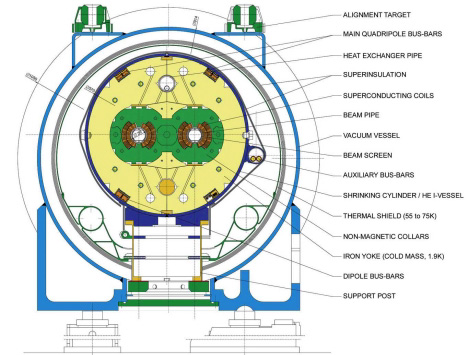
\includegraphics[width=.7\textwidth]{Detector_plots/LHC-double-bore-magnet.jpg}
		\caption{ Double-bore magnet configuration of the LHC 
		superconducting magnets~\cite{rossi2003lhc}.}
		\label{fig:double-bore-magnet}
		\end{centering}
	\end{figure}

	Due to the technical difficulties to install 
	two separate rings in such small space,
	LHC adopted the twin-bore magnet design~\cite{rossi2003lhc}, 
	as shown in Figure~\ref{fig:double-bore-magnet}.
	It was proposed by John Blewett at the Brookhaven 
	laboratory in 1971 first for
	cost consideration~\cite{Blewett:1971zzb},
	but in the case of the LHC the overriding reason for adopting this solution
	is the lack of space in the tunnel. 

	The aim of the LHC is to reveal the physics beyond
	the Standard Model with centre of mass 
	collision energies of up to 14 TeV.
	The number of events per second generated in the LHC collisionsis given by:
	\[
		N_{event} = L\sigma_{event},\]
	where $\sigma_event$ is the cross section 
	for the event under study and $L$ the machine luminosity. 
	The machine luminosity depends on the beam parameters 
	and can be written for a Gaussian beam distribution as:
	\[
	L = \frac{N_b^2 n_b f_{rev} \gamma_r}{4\pi \epsilon_n \beta*} F,
	\]

	where $N_b$ refers to the number of particles per bunch,
	$n_b$ number of bunches per beam,
	$f_{rev}$ revolution frequency, 
	$\gamma_r$ relativistic gamma factor, 
	$\epsilon_r$ normalized transverse beam emittance, 
	$\beta*$~beta function at the collision point which
	describes the size of the beam, 
	and	$F$ refers to the geometric luminosity reduction factor due to the 
	crossing angle at the interaction point~(IP).

	The two high luminosity experiments, ATLAS and CMS are
	both aiming at a peak luminosity of $L$ = $10^{34}cm^2s^1$ for proton operation.
	The two low luminosity experiments: LHCB for 
	B-physics, is aiming at a peak luminosity of $L$ = $10^{32}cm^2s^1$, 
	and the dedicated ion experiment, ALICE, is aiming at apeak luminosity of
	$L$ = $10^{27}cm^2s^1$ for nominal lead-lead ion operation.


	\begin{figure}[bht]
		\begin{centering}	
		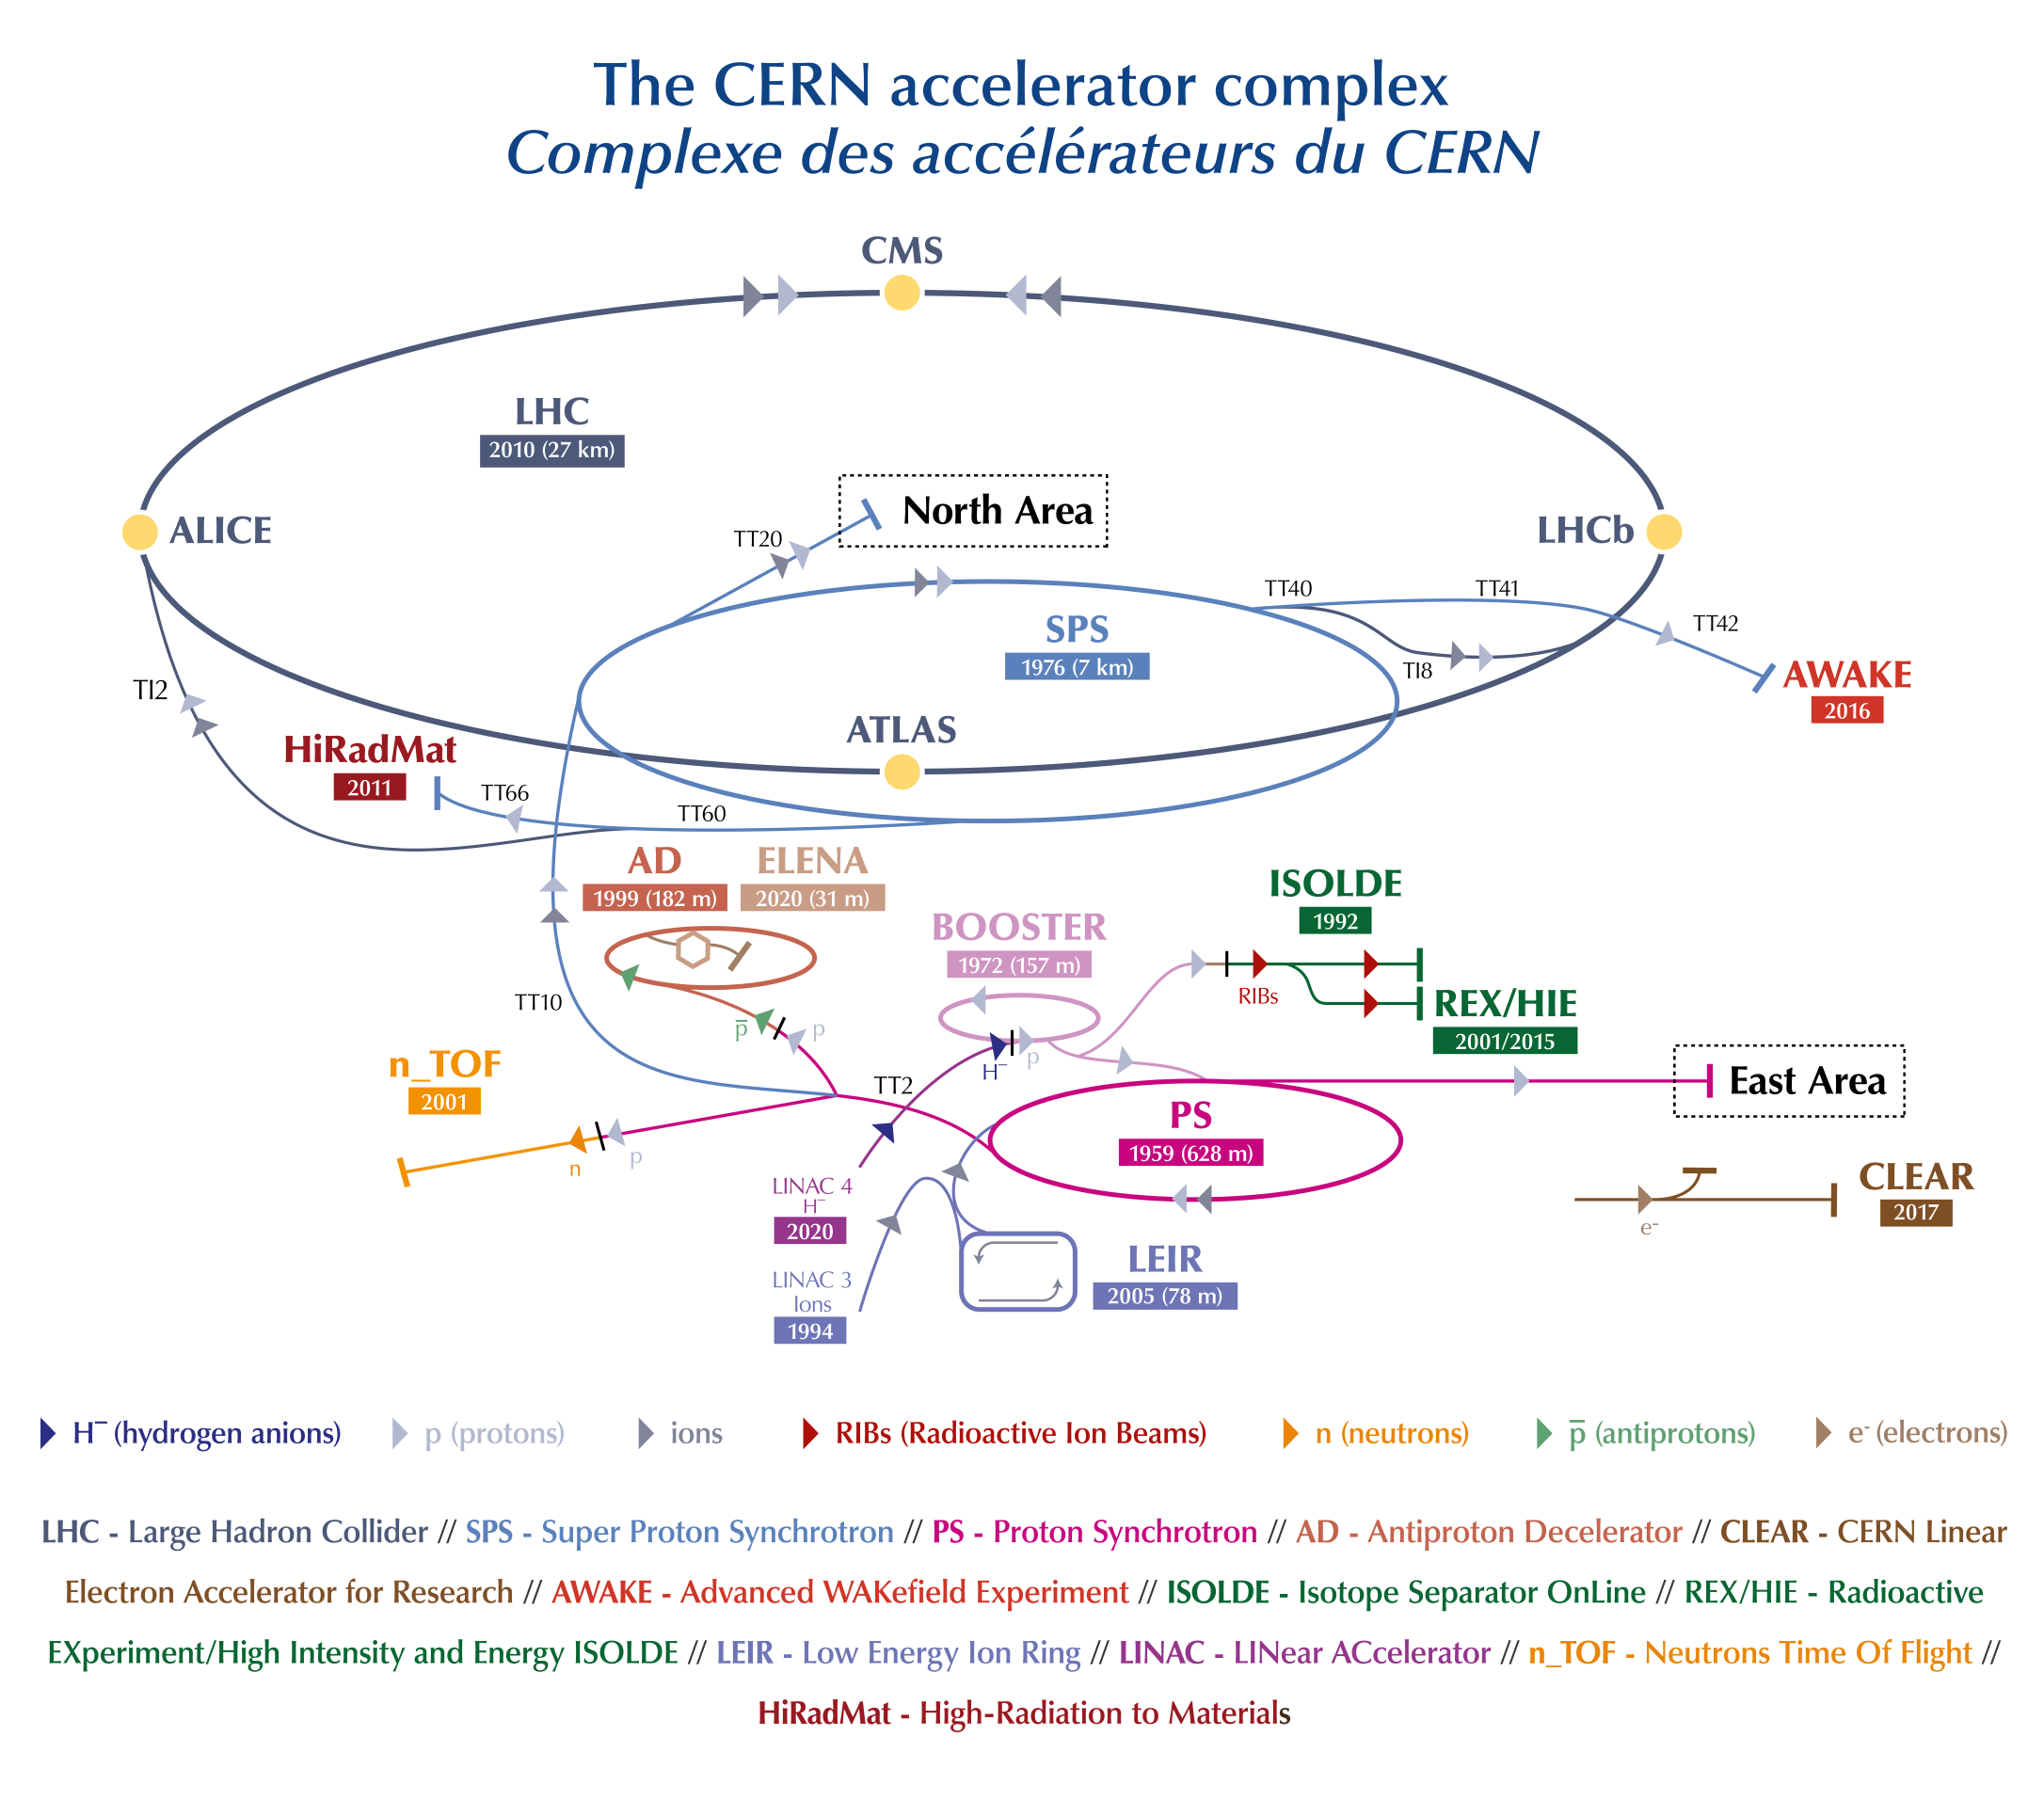
\includegraphics[width=.75\textwidth]{Detector_plots/accelerator_complex_smaller.png}
		\caption{The LHC is the last ring (dark blue line) in a complex chain of 
		particle accelerators. The smaller machines are used in a chain to help boost 
		the particles to their final energies and provide beams to a whole set of smaller experiments.
			}
		\label{fig:accelerator_complex}
		\end{centering}
	\end{figure}
	The proton beams are designed to carry energy of the order of a few TeV.
	To reach such high energy, a series of acceleration is required for the beams before
	entering the LHC ring. The protons are supplied by the injector chain 
	Linac2 — Proton Synchrotron Booster (PSB) — Proton Synchrotron (PS) — Super Proton Synchrotron (SPS), 
	as shown in Figure~\ref{fig:accelerator_complex}, 
	reaching an energy of 450 GeV when leaving the SPS. 
	Each proton beam contains 2808 ``bunches'' of approximately 
	$1.15 \times 10^{11}$ protons, arranged in 
	``trains'' of bunches with 72 bunches each ``carriage''. 
	Inside the ``carriage'', each beam has a spacing of 24.95 ns and between each 
	``carriage'' there is a gap of \~ 320 ns. 
	The beams are required to have well defined transverse and longitudinal emittance. 


	\subsubsection{Runs and results}
	\label{sec:runs and results}
	Following the downtime after an incident in one of the main dipole circuits 
	during the first commissioning in 2008~\cite{lebrun2009report},
	the operation restarted at lower beam energy to minimize the risk. 
	Therefore, the first proton run (2010-2013)~\cite{alemany2013operation} was
	carried out at 3.5–4 TeV (centre of mass energy 7-8 TeV). Furthermore, a bunch spacing
	of 50 ns was used instead of the nominal 25 ns. 
	This implied fewer bunches with larger intensity and hence a 
	high peak luminosity (0.8 $\times$ 10$^{34}$ cm$^{-2}$s$^{-1}$ still smaller than
	the nominal 10$^{34}$ cm$^{-2}$s$^{-1}$ luminosity) but larger than nominal pileup. 
	Run 1 resulted in about 30~\fb of proton data and important physics results,
	most notably the discovery of the Higgs boson~\cite{HIGG-2012-27},~\cite{HIGG-2012-28}.
	Run 1 was followed by a long shutdown (LS1, 2013–2014)
	with a large number of consolidation and upgrade activities~\cite{bordry2013first}. 	
	The bus-bar splices between the superconducting magnets were improved, 
	in order to make sure that the LHC could operate at higher energy 
	without risk of repeating the 2008 incident. 

	\begin{figure}[bht]
		\begin{centering}	
		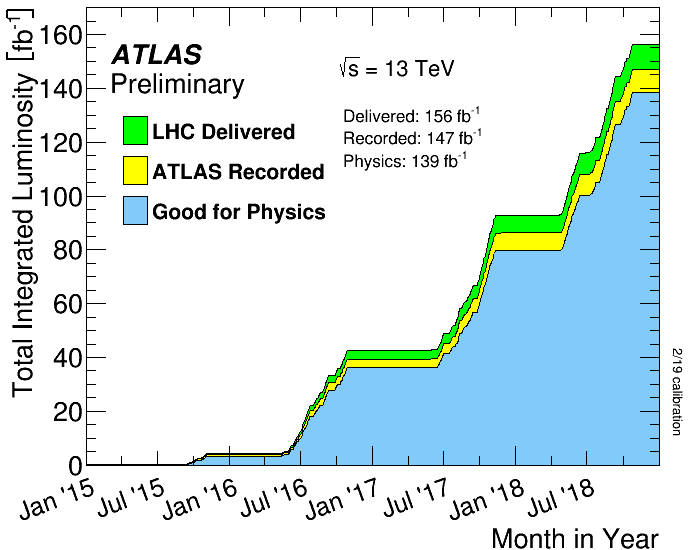
\includegraphics[width=.4\textwidth]{Detector_plots/Run2_lumi.png}
		\caption{Cumulative luminosity versus time delivered to 
		ATLAS (green), recorded by ATLAS (yellow), and certified to be 
		good quality data (blue) during stable beams for pp collisions 
		at 13 TeV centre-of-mass energy in Run 2. 
			}
		\label{fig:Run2_lumi}
		\end{centering}
	\end{figure}
	
	Run 2 (2016-2018) was carried out
	at 6.5 TeV (center of mass energy 13 TeV)~\cite{LHC-Run2-Operation}. 
	As shown in Figure~\ref{fig:Run2_lumi}, out of the 156~\fb 
	of data LHC has delivered, the ATLAS detector has recorded 
	147~\fb and \lumi of data is certified to be good quality data.
	The delivered luminosity accounts for the luminosity delivered from the start of 
	stable beams until the LHC requests ATLAS to put the detector in a 
	safe standby mode to allow a beam dump or beam studies. 
	The recorded luminosity is slightly smaller than the delivered luminosity, due 
	to the inefficiency of the Data Acquisition (DAQ) and the so called ``warm start'': 
	when the stable beam flag is raised, 
	the tracking detectors undergo a ramp of the high-voltage and, 
	for the pixel system, turning on the pre-amplifiers. 
	More details of the ATLAS detector can be found in the following sections. 
	The recorded data is checked carefully to exclude possible hardware or software  issues. 
	This is achieved by monitoring detector-level quantities 
	and reconstructed collision event characteristics at key stages of the data processing chain.
	This procedure led to high efficiency of good quality data: 95.6\%~\cite{aad2020atlas}.	

	\begin{figure}[bht]
		\begin{centering}	
		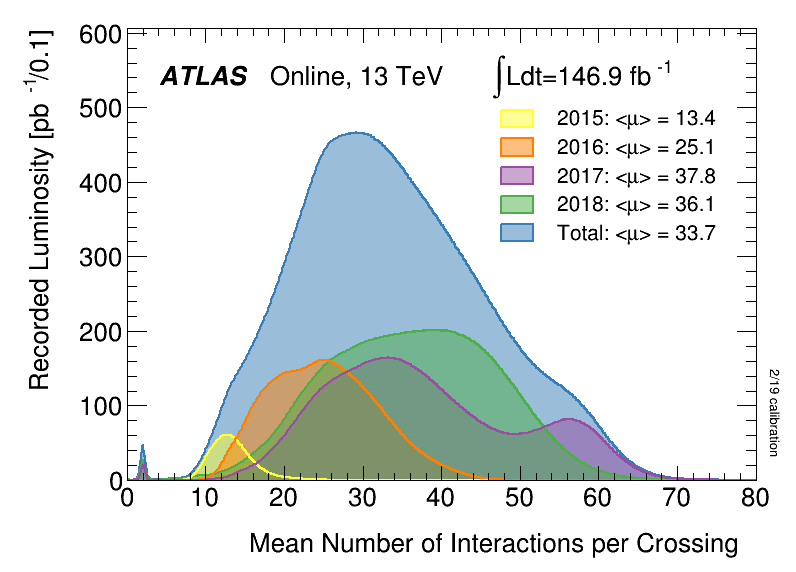
\includegraphics[width=.4\textwidth]{Detector_plots/Run2_pileup.png}
		\caption{ Shown is the luminosity-weighted distribution of the mean number of 
		interactions per crossing for the Run 2 data. All data recorded by ATLAS during 
		stable beams is shown, and the integrated luminosity and 
		the mean mu value are given in the figure. 
			}
		\label{fig:Run2_pileup}
		\end{centering}
	\end{figure}

	In this thesis the \lumi data recorded by the ATLAS detector of Run 2 is used.
	The nominal bunch spacing of 25 ns was used, with slightly less bunches (2500) each beam.
	The LHC experts have continually improved the running scenario to increase the luminosity,
	and during Run 2 the luminosity surpassed the designed luminosity by a factor of 2. 
	As well as improving the instantaneous luminosity, the availability of the machine
	was dramatically improved during Run 2 which is an important factor enabling the high efficiency 
	of good quality data as mentioned above.
	During Run 2, the machine was providing physics collisions during 50\% of 
	the allocated physics time, which is very impressive for a super conducting collider. 
	An important parameter for the LHC experiments is the pileup, 
	which is determined by the luminosity per bunch, and is a measure of 
	the number of inelastic pp interactions that occur per bunch crossing. 

	Higher pileup gives more luminosity (for a fixed number of bunches) 
	but makes physics analysis more difficult due to the signals in the detector 
	from the additional interactions. The distribution of the recorded luminosity over
	the pileup is shown in Figure~\ref{fig:Run2_pileup}. It's a challenging task for the 
	trigger and reconstruction algorithms to achieve robustness under such high pileup 
	condition.

	\begin{figure}[bht]
		\begin{centering}	
		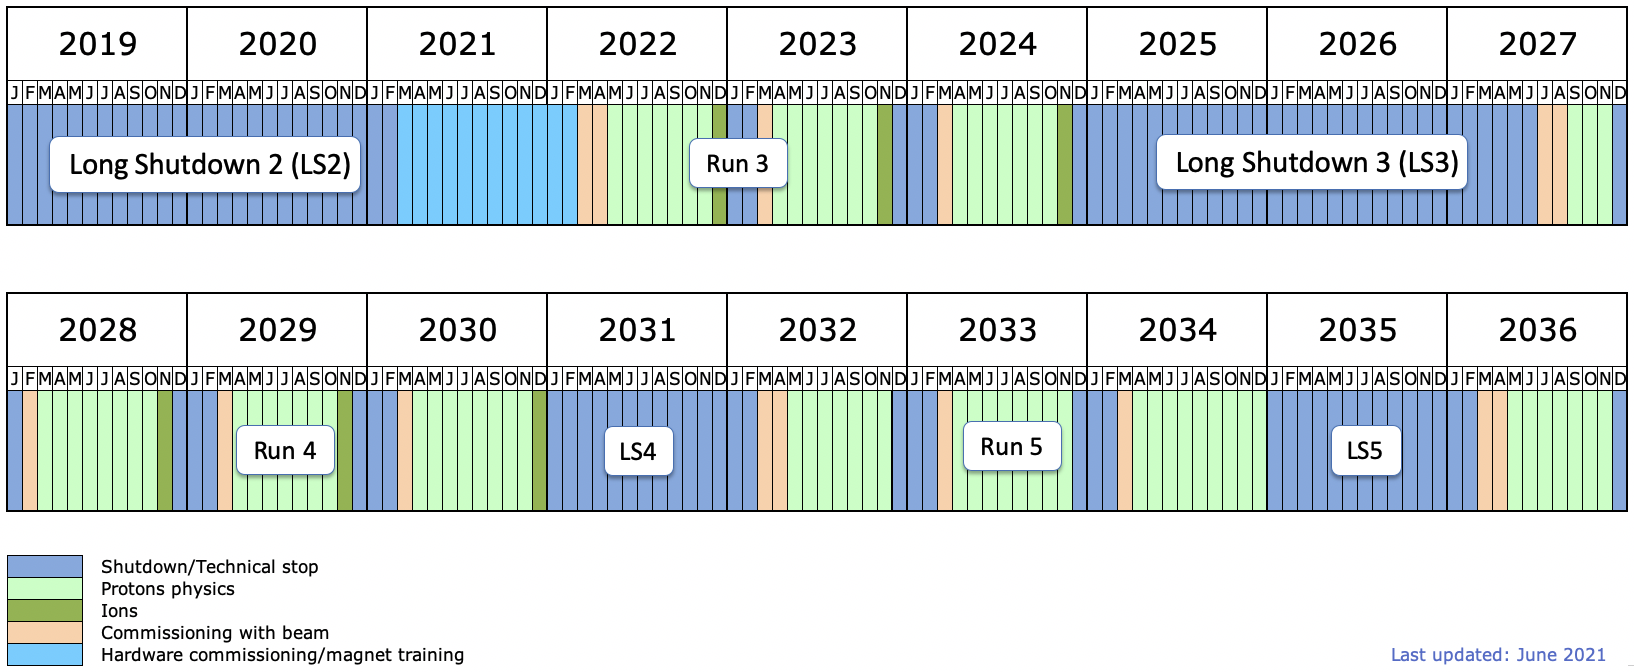
\includegraphics[width=.8\textwidth]{Detector_plots/LHC-longterm-schedule.png}
		\caption{Longer term LHC operation schedule.% [source: https://lhc-commissioning.web.cern.ch/schedule/LHC-long-term.htm]
			}
		\label{fig:LHC-longterm-schedule}
		\end{centering}
	\end{figure}
	
	\begin{figure}[bht]
		\begin{centering}
		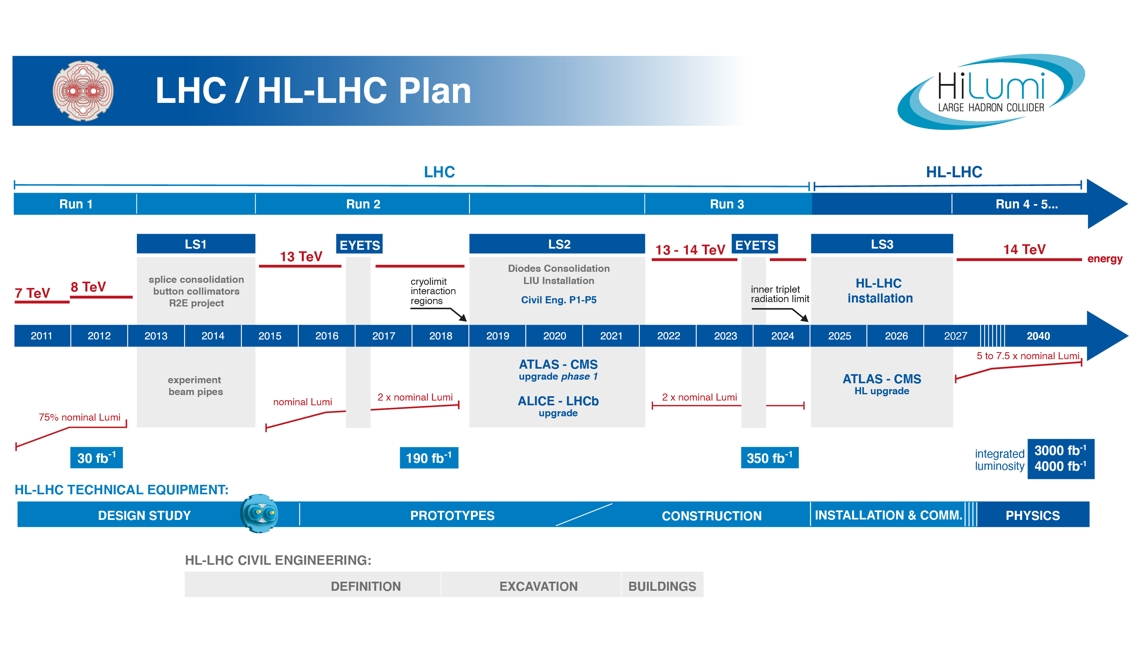
\includegraphics[width=.65\textwidth]{Detector_plots/LHC-schedule-lumi.jpg}
		\caption{LHC operation schedule and luminosity targets.  %[source:project HL-LHC, https://project-hl-lhc-industry.web.cern.ch/content/project-schedule ]
			}
		\label{fig:LHC-schedule-lumi}
		\end{centering}
	\end{figure}
	The LHC operation and shutdown schedule is shown 
	in Figure~\ref{fig:LHC-longterm-schedule}
	and Figure~\ref{fig:LHC-schedule-lumi}.
	The operation of CERN’s accelerators is subject to scheduled shutdowns 
	to allow important repair and upgrade work to take place. 
	The present shutdown, LS2, is devoted to preparations for Run 3 of the LHC, 
	which will have an integrated luminosity equal to the two previous runs combined, 
	and for the High-Luminosity LHC (HL-LHC), 
	the successor to the LHC, which will begin operation at the end of 2027,
	and eventually generate 10 times the integrated luminosity to
	all Run 1, 2, 3 combined!
	
	The LS2 schedule has had to be modified due to the COVID-19 pandemic, 
	which the new schedule anticipates that the first test beams will 
	circulate in the LHC 
	at the end of September 2021, four months later than the date 
	planned before the COVID-19 crisis, 
	to give the LHC’s main experiments – ATLAS, CMS, ALICE and LHCb – 
	time to prepare their own upgrade. 
	Run 3 of the LHC will begin at the start of March 2022.
	% No changes have been made to the schedule beyond 2022.
	The third long shutdown (LS3) will begin at the 
	start of 2025 and end in mid-2027. 
	This is when the equipment for the HL-LHC and 
	its experiments will be installed. 
	





\subsection{The ATLAS Detector}

\begin{figure}[bht]
	\begin{centering}	
	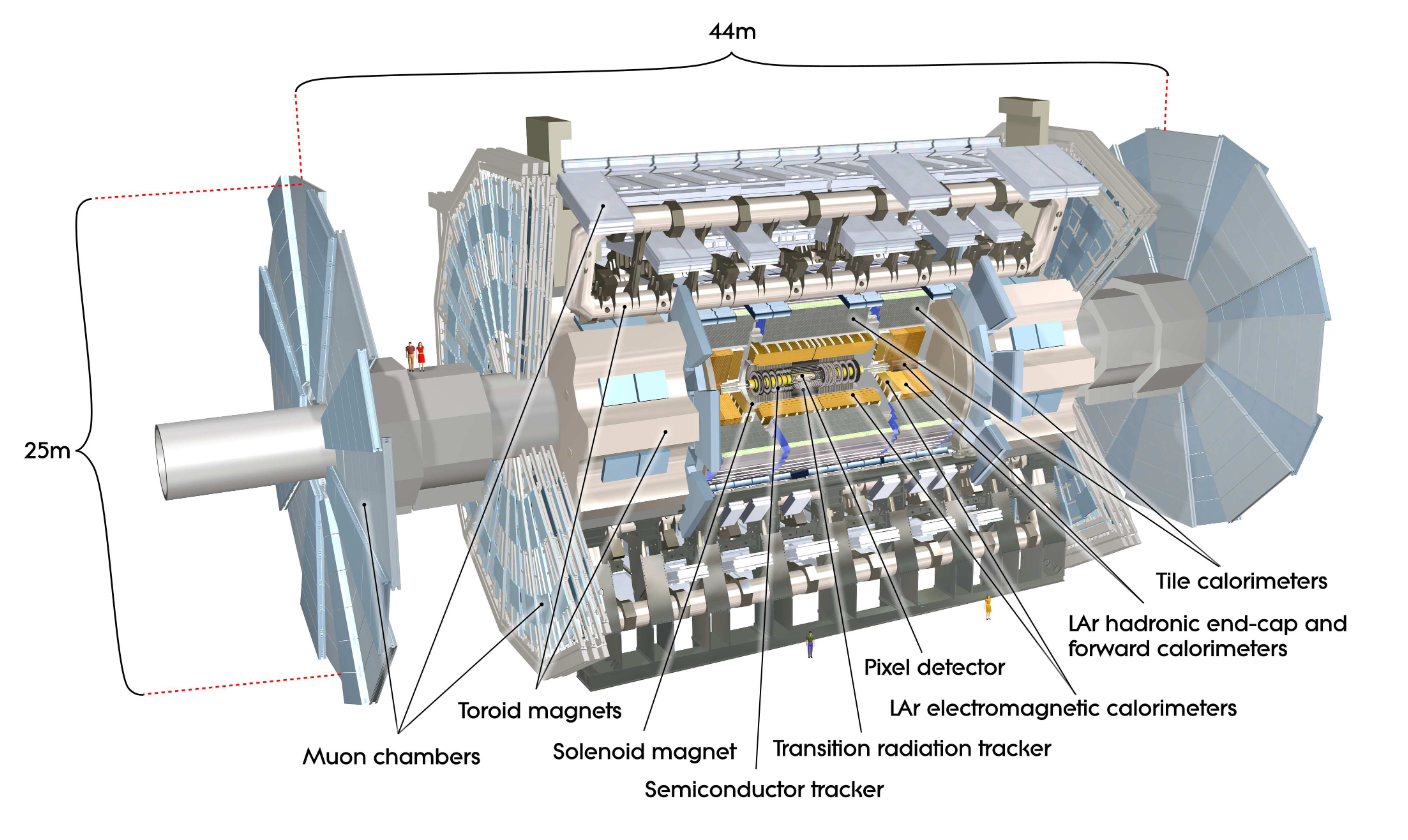
\includegraphics[width=.65\textwidth]{Detector_plots/Cut-away-view-of-the-ATLAS-detector.png}
	\caption{Cut-away view of the ATLAS detector. 
	The dimensions of the detector are 25 m in
	height and 44 m in length. The overall weight 
	of the detector is approximately 7000 tonnes.
		}
	\label{fig:ATLAS_cut_away}
	\end{centering}
\end{figure}

ATLAS is one of the 
two general purpose detectors built for probing proton-proton 
collision. This detector represents the work of a large collaboration 
of several thousand physicists, engineers, technicians,
and students over a period of fifteen years of dedicated 
design, development, fabrication, and installation.
A overall layout of the detector is shown in Figure~\ref{fig:ATLAS_cut_away}.

The high interaction rates, radiation doses, particle 
multiplicities and energies, as well as the
requirements for precision measurements have set strigent
standards on the design of the ATLAS detector. 
Therefore the ATLAS detector is designed to fufiled the following 
requirements:

\begin{table}[thb]
	\centering
	\small
	\setlength\tabcolsep{5pt} 
	\begin{tabular}{|c|c|c|c| }
	\hline
	\multirow{2}{*}{Detector component}&\multirow{2}{*}{Required resolution} & \multicolumn{2}{c|}{$\eta$ coverage} \\ \cline{3-4}
	
	  & & Measurement &  Trigger\\ 
	 \hline
	Tracking         &    $\sigma_{p_T}/p_T = 0.05\%p_T\bigoplus 1\% $        &  $\pm 2.5$  & None \\  
	\hline
	EM calorimetry      &  $\sigma_E/E = 10\%/E\bigoplus 0.7\% $       & $\pm 3.2$ &  $\pm 2.5$\\
	\hline
	Hadronic calorimetry (jets)   &        & &      \\
	\hline
	barrel and end-cap &  $\sigma_E/E = 50\%/E\bigoplus 3\% $       & $\pm 3.2$ &  $\pm 3.2$\\
	forward   &  $\sigma_E/E = 100\%/E\bigoplus 10\% $       & $ 3.1 < |\eta | < 4.9 $ &  $3.1 < |\eta | < 4.9 $\\
	\hline
	Muon spectrometer  &    $\sigma_{p_T}/p_T = 10\%$ at \pt $=\ 1$ TeV        &  $\pm 2.7$  & $\pm 2.4$ \\  
	\hline
	\end{tabular}
	\vspace{0.2cm}
	\caption{General performance goals of the ATLAS detector. Note that, for high-\pt\ muons,
	the muon-spectrometer performance is independent of the inner-detector system. The units for E
	and \pt\ are in GeV \cite{PERF-2007-01}.}
	\label{tab:ATLAS_performance}
\end{table}




\begin{itemize}
\item
The detector requires fast, radiation-resistant  
electronics and sensor elements and high detector granularity
to meet the requirements due to the high frequency of collision,
high particle fluxes and high radiation environment of the
detector.


\item
Due to the geometry of the detector, to collect most of the 
collision data, large acceptance in pseudorapidity (which will be defined
in the next subsection: \ref{sec:detector coordinate}) 
with almost full azimuthal angle coverage is required.


\item
Good energy and momentum resolution are required to 
enable accurate physical objects reconstruction. 
The high resolution of energy can be obtained 
with very good electromagnetic (EM) calorimetry for 
electron and photon identification and measurements,
complemented by full-coverage hadronic calorimetry 
for accurate jet and missingtransverse energy measurements.


\item
For offline tagging of $\tau$-leptons and b-jets, vertex 
detectors close to the interaction region are 
required to observe secondary vertices.


\item
Good muon identification and momentum resolution 
over a wide range of momenta and the ability 
to determine unambiguously the charge of high 
\pt\ muons are fundamental requirements.


\item

Triggering with high efficiency on \pt\  
objects with sufficient background rejection is a 
prerequisite to achieve an acceptable trigger rate 
for most physics processes of interest.
\end{itemize}


The main performance goals of the detector are 
listed in Table \ref{tab:ATLAS_performance}. 


\subsubsection{Coordinate system}
	\label{sec:detector coordinate}



	The ATLAS coordinate system is a right-handed Cartesian system
	with the nominal interaction point 
	defined as the origin of the coordinate system,  
	while the beam direction defines the z-axis and 
	the x-y plane is transverse to the beam direction.  
	The positive x-axis is defined as pointing from 
	the interaction point to the centre of the
	LHC ring and the positive y-axis is defined as 
	pointing upwards, as shown in Figure~\ref{fig:ATLAS_coordinate_system}. 

	\begin{figure}[bht]
		\begin{centering}	
		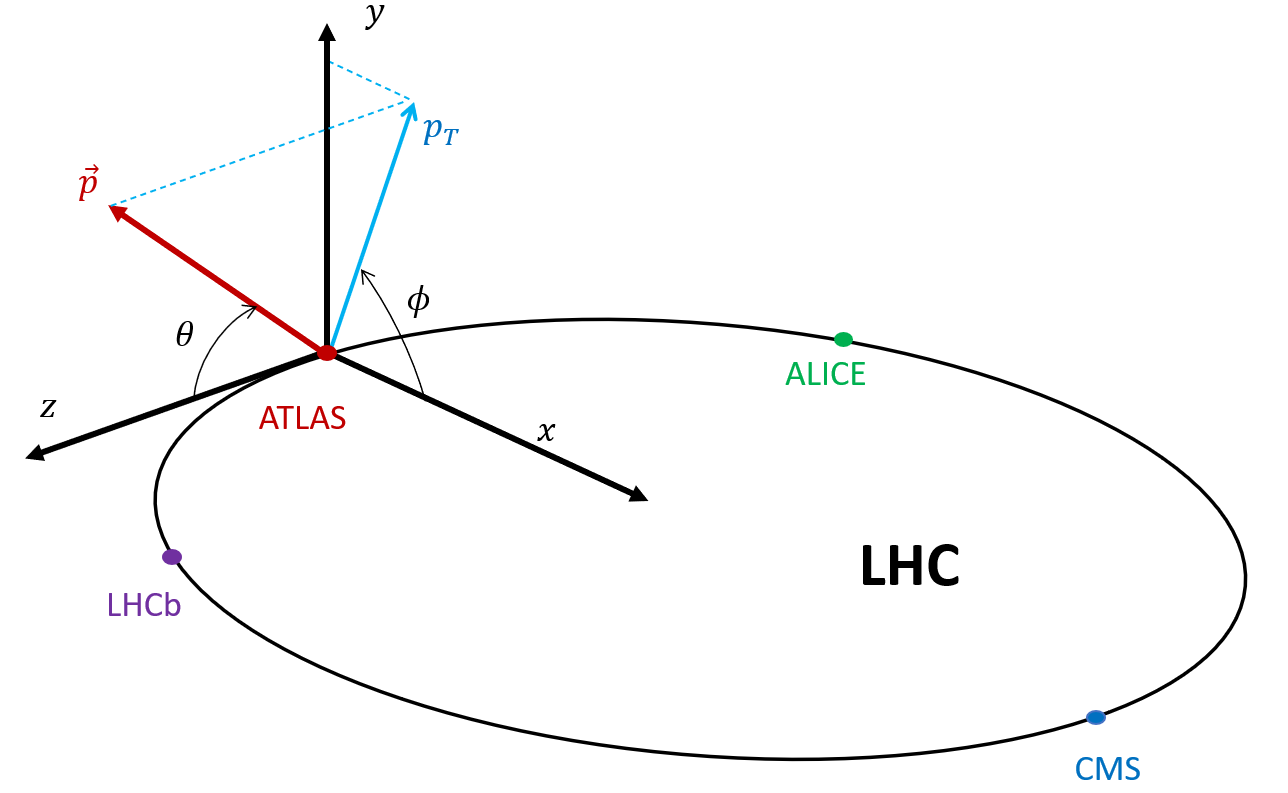
\includegraphics[width=.55\textwidth]{Detector_plots/ATLAS coordinate system.png}
		\caption{Illustration of the coordinate systems 
		used at the ATLAS experiment in the geographical context of the LHC.
			}
		\label{fig:ATLAS_coordinate_system}
		\end{centering}
	\end{figure}

	The azimuthal angle $\phi$ 
	is measured as usual around the beam axis, and 
	the polar angle $\theta$ is the angle from the beam axis.  
	In high energy physics, it's more common to use the 
	pseudorapidity instead of the
	polar angle $\theta$, defined as:

	\[ \eta = -ln\ tan(\theta/2). \]

	In the case of highly relativistic particles
	(which is the comman case in high energy physics), 
	the pseudorapidity approaches the rapidity, 

	\[ y=1/2ln[(E+p_z)/(E-p_z)], \]

	with E the energy of the particle, m its mass 
	and $p_z$ the momentum along the z axis.

	There are two main reasons for using pseudorapidity.
	The first reason is that the rapidity is invariant
	under Lorentz transformation, while capturing 
	the characteristic of the particle direction of travel:
	$y \rightarrow \pm \infty $ when the particle is  
	travelling close to the beam pipe (positive for along the
	beam pipe, negative for the opposite direction) and
	$y \rightarrow 0$ when $p_z$ is small.
	While the second reason is that due to the limited
	angle coverage of the detector, it's usually hard
	to determine the total energy and the momentum 
	along the z axis, especially when the direction of 
	the particles are close to the beam pipe. 
	While the pseudorapidity is determined only by
	the polar angle, which is much easier and faster 
	to compute. 

	The transverse momentum \pt, the transverse energy
	$E_T$, and the missing transverse energy $E_{miss}^T$ (MET) 
	are defined in the x-y plane unless stated otherwise.  
	The distance $\Delta R$ in the pseudorapidity-azimuthal angle 
	space is defined as:

	\[\Delta R = \sqrt{\Delta \eta^2+\Delta\phi^2}.\]

\subsubsection{Magnets}


	ATLAS has a unique hybrid system of four large superconducting 
	magnets~\cite{ATLAS-TDR-06}. This magnetic system is 22 m in diameter and 26 m in length, 
	with a stored energy of 1.6 GJ.
	Figure~\ref{fig:ATLAS_cut_away} shows the general layout, 
	the four main layers of detetors and the four superconducting 
	magnets which provide the magnetic
	field over a volume of approximately 12000 $m^3$.
	
	\begin{figure}[bht]
		\begin{centering}	
		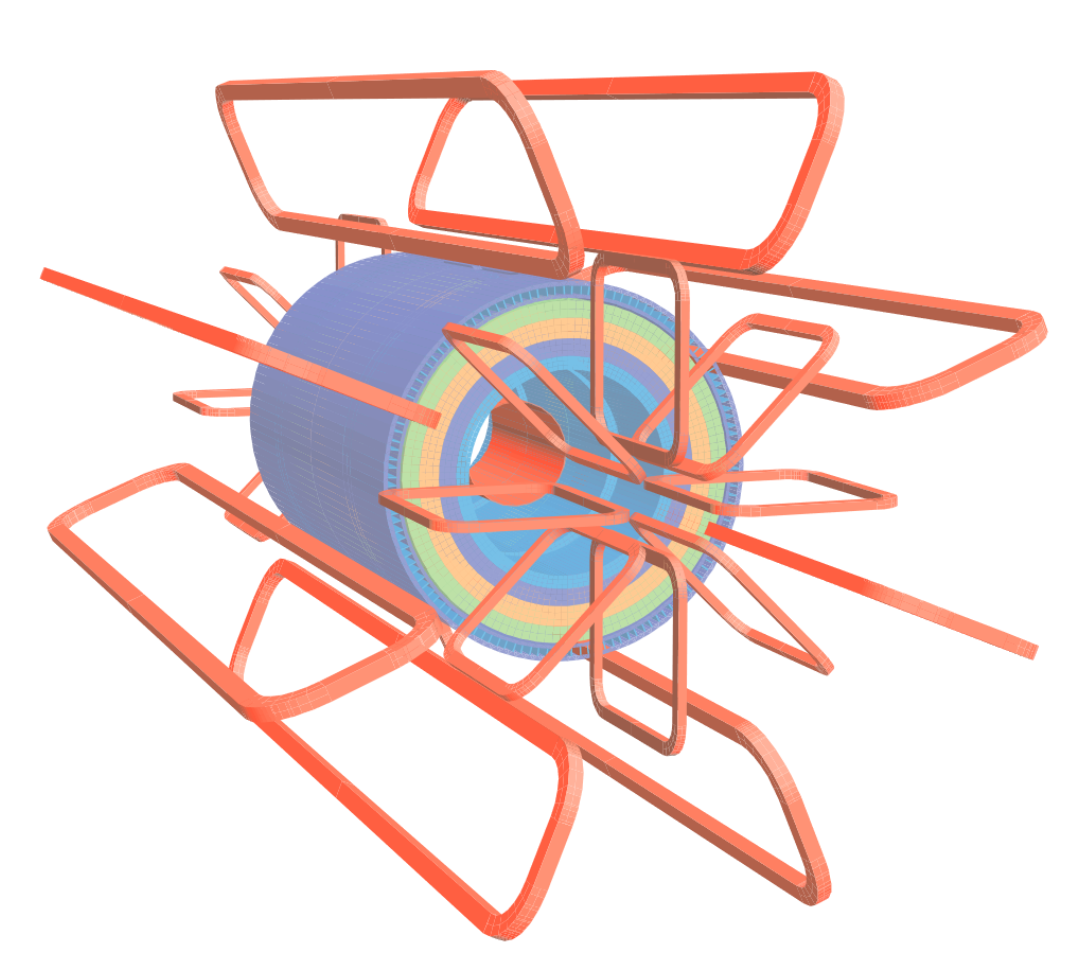
\includegraphics[width=.36\textwidth]{Detector_plots/ATLAS magnets.png}
		\caption{Geometry of magnet windings and
		tile calorimeter steel.	}
		\label{fig:ATLAS_magnets}
		\end{centering}
	\end{figure}

	The spatial arrangement of the coil windings is shown in 
	Figure~\ref{fig:ATLAS_magnets}. 
	The ATLAS magnet system consists of two parts:
	\begin{itemize}
		\item a solenoid, which is aligned on the beam axis and 
		provides a 2 T axial magnetic field in the z-direction. 
		For the inner detector, while minimising 
		the radiative thickness in front of the	barrel 
		electromagnetic calorimeter;
		\item  a barrel toroid and two end-cap toroids, 
		which produce a	toroidal magnetic field of approximately 
		0.5 T and 1 T for the muon detectors in the central 
		and end-cap regions, respectively. 
		The barrel toroid generates the magnetic field in the central zone 
		of the muon spectrometer, along the tangential direction of 
		the circumferences centered on the z-axis ($\phi$ direction). 
		The end-cap toroids are two smaller toroids designed to 
		provide the magnetic field in the forward areas of 
		the muon spectrometer. 
		
		
	\end{itemize}		
	Therefore in the ATLAS magnetic system, tracks in the inner detector
	is bended in the $\phi$ direction, while in the muon spectrometer 
	in the $\theta$ direction.


\subsubsection{Inner detector}	
	The innder detector~\cite{ATLAS-TDR-04} consists of three parts: the pixel detector~\cite{ATLAS-TDR-11}
	and	the insertable B-Layer (IBL)~\cite{ATLAS-TDR-19} (as one part),
	the silicon micro strip tracker (SCT)~\cite{}{ATLAS-TDR-04}, the transition radiation
	tracker (TRT)~\cite{ATLAS-TDR-04}. 
	Figure~\ref{fig:inner_detector} shows a 
	charge track traverses the sensors and structural
	elements. 
	\begin{figure}[bht]
		\begin{centering}	
		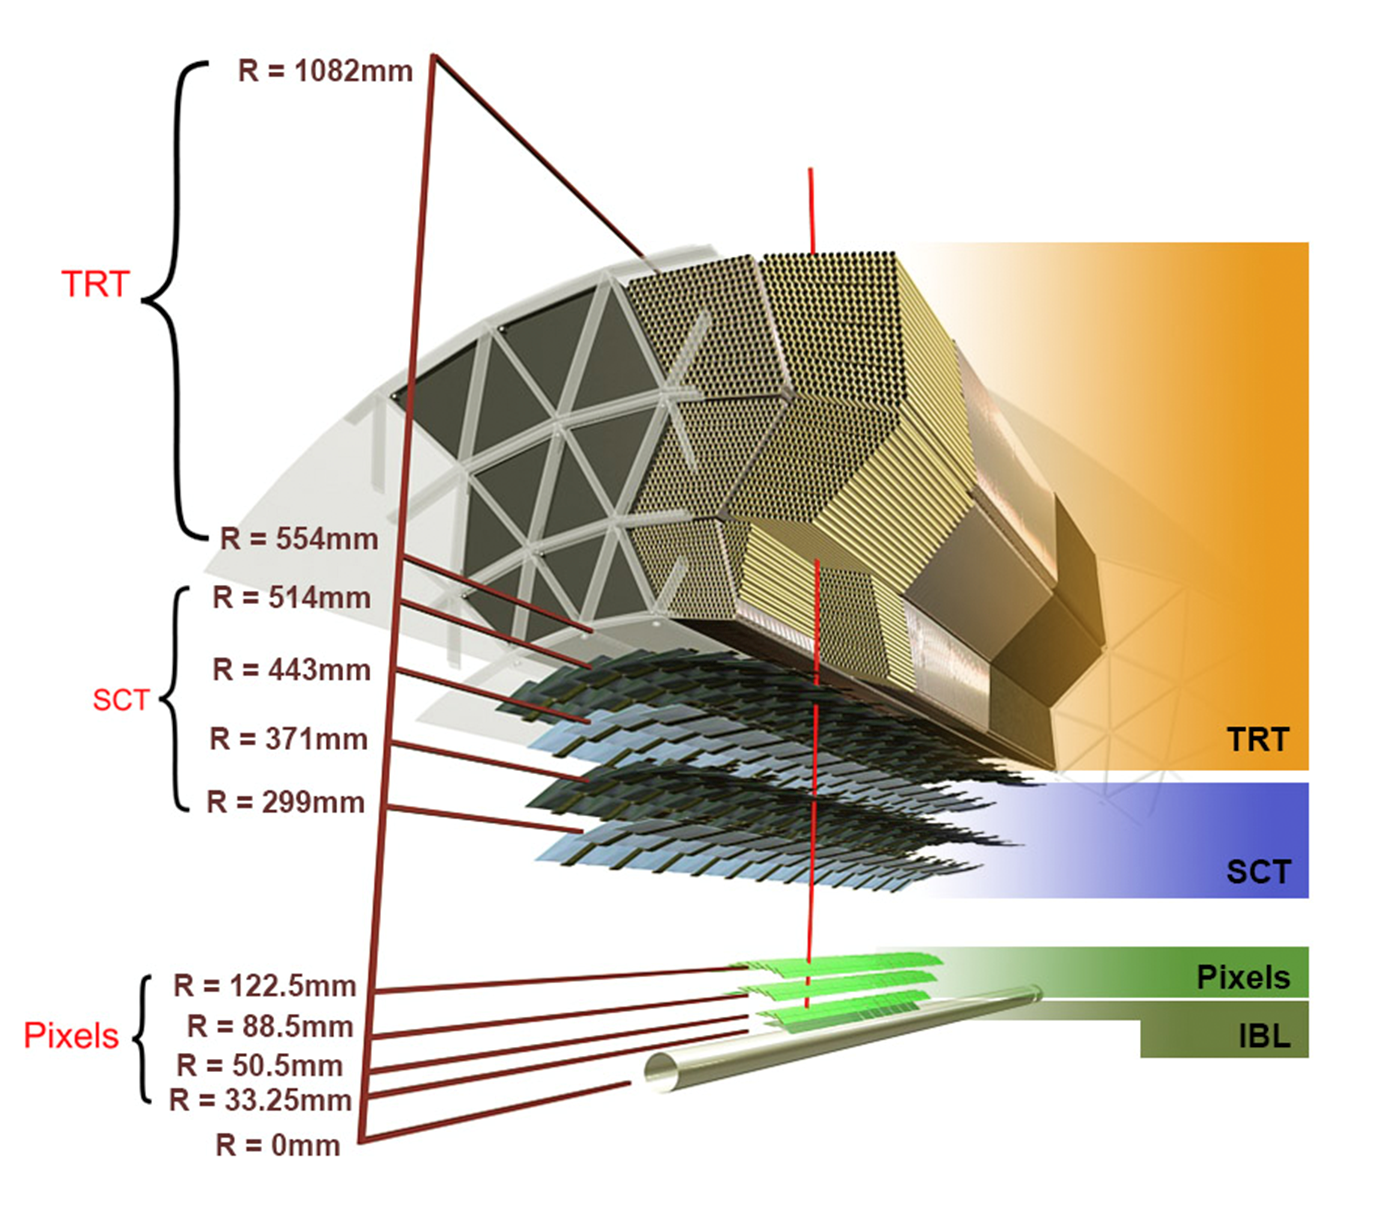
\includegraphics[width=.55\textwidth]{Detector_plots/Inner detector.png}
		\caption{Cut-away view of the inner detector.}
		\label{fig:inner_detector}
	\end{centering}
	\end{figure}
	The track traverses successively the beryllium
	beam-pipe, the four cylindrical silicon-pixel layers 
	with individual 
	sensor elements of 50$\times$400 $\mu m^2$, the four cylindrical double 
	layers of barrel SCT of pitch 80 $\mu m$, 
	and approximately 36 axial straws of 4 $mm$ diameter 
	contained in the barrel TRT
	modules within their support structure.
	\begin{itemize}
		\item \textbf{Pixel detector and IBL}\\
	The silicon pixel detector is the closest ATLAS 
	component to the collision. It is composed of layers of
	silicon pixels and designed to have a very 
	high granularity for reconstructing primary 
	and secondary interaction vertices. 
	The detector layers are formed of silicon sensor modules and 
	in total there are approximately 92 million pixels 
	(consequently, 92 million readout channels) in the system.
	It consists of three cylindrical layers in the 
	barrel region, positioned at the radial distances of 
	50.5, 88.5 and 122.5 mm 
	and on disks perpendicular to the beams in the end-caps at the
	longitudinal distances of 49.5, 58.0 and 65.0 mm. 
	% The B-layer, placed at a distance of 50.5mm, plays 
	% an important role in detecting secondary vertices 
	% for the identification of jets coming from 
	% b-quark hadronisation (\bjets). 
	In 2014, during the first LHC long shutdown, a fourth pixel 
	layer was installed inside the existing detector, 
	the insertable B-Layer (IBL) at a radius of 33 mm 
	from the beam axis.
	The new pixel layer provides an 
	additional space point very close to the interaction point, 
	which significantly improves the identification of jets coming from 
	b-quark hadronisation (\bjets). 
	\item \textbf{SCT} \\
	The next constituent of the inner detector is the SCT, 
	which consists of four layers of strips located axially on the 
	beam direction in the barrel region and placed along the 
	\mbox{R-direction} in the end-cap region. 
	Each layer of strip is glued back to back with an angle of
	40 mrad. The spatial resolution of the sensor is 
	$\sigma_\phi = 17\ \mu m$ in the bending direction ($R-\phi$)
	and $\sigma_\phi = 580\ \mu m$ in the z (barrel) and R (end-cap) direction. 
	\item \textbf{TRT} \\
	The most external part of the inner detector is the TRT. 
	It is a straw drift tube tracker, with additional electron identification
	capabilities from transition radiation. It consists of
	modules of 4 mm diameter straws, filled with a mixture of gas of
	70\% Xe, 27\% CO2 and 3\% O2 immersed in a polypropylene radiator.
	Up to 73 straw layers of straws are interleaved with fibres in the barrel
	and 160 starw planes are interleaved with foils in the end-cap. 
	All charged tracks with \pt\ $> 0.5$ GeV and $|\eta| < 2.0$ will traverse 
	at least 36 straws, except in the
	barrel-end-cap transition region ($0.8 < |\eta|< 1.0$), 
	where this number decreases to a minimum of 22 crossed straw.
	The TRT measures the track position only in the bending direction
	($R-\phi$), with a spatial resolution of $\sigma_\phi = 130\ \mu m$.
	The TRT contributes significantly to the pattern recognition and 
	momentum reconstruction, depsite the low resolution compared to the 
	silicon tracker and the lack of a measurement along the z axis. 
	This is the result of the large number of measurements and longer
	measured track length. In addition, the TRT provides extra ability to 
	identify elecctrons due to the polypropylene fibres (foils) in the barrel
	(end-cap) emit photons when a charged particle traverses the boundaries of
	the material. These photons are then absorbed by the Xenon gas mixture, which
	the intensity depends on gamma factor of the traversing particle. 
	This information can then be exploited for eletron/pion discrimination.
	\end{itemize}

	\subsubsection{Calorimeter system}



	\begin{figure}[bht]
		\begin{centering}	
		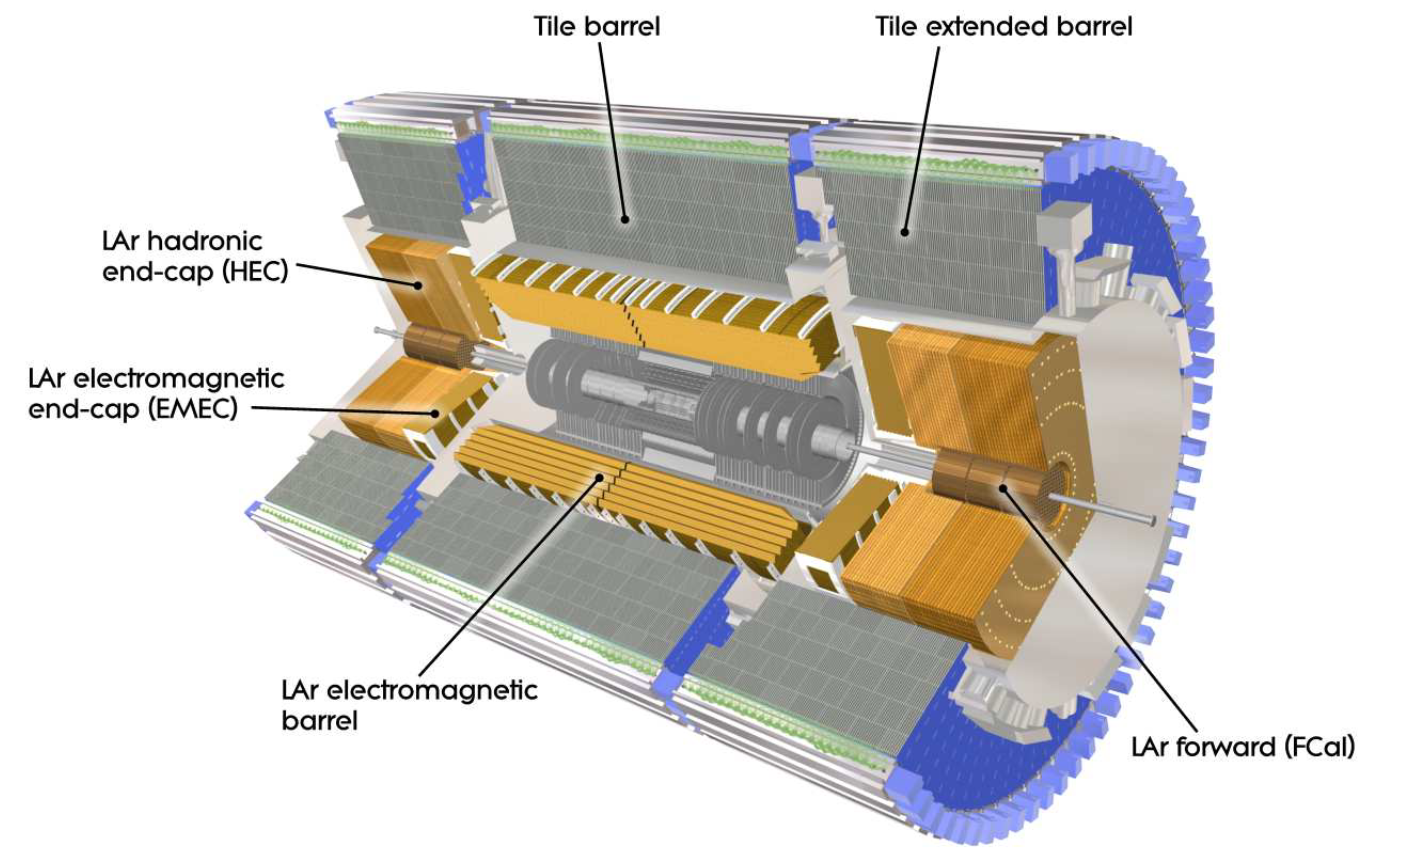
\includegraphics[width=.6\textwidth]{Detector_plots/calo.png}
		\caption{Cut-away view of the ATLAS calorimeter system.}
		\label{fig:calo}
		\end{centering}
	\end{figure}

	The ATLAS calorimeters~\cite{ATLAS-TDR-01}
	are sampling calorimeters, meaning
	different material are used for the absorber and the active part.
	A cut-away view of the calorimeters is shown in Figure~\ref{fig:calo}.
	These calorimeters cover the range $|\eta|$< 4.9, using 
	different techniques suited to the widely varying requirements 
	of the physics processes of interest and of the radiation environment
	over this large $\eta$-range. Over the $\eta$ region matched to 
	the inner detector, the fine granularity of	the EM calorimeter 
	is ideal for precision measurements of electrons and photons. The
	coarser granularity of the rest of the calorimeter is sufficient 
	for the jet reconstruction and $E_{miss}^T$ measurements.

	The electromagnetic and hadronic showers must be contained in the 
	calorimeter to avoid punch-through into the muon system. 
	The calorimeter depth is hence an important design consideration. 
	The total thickness of the EM calorimeter is greater than
	22 radiation lengths ($X_0$) in the barrel and greater than 
	24 $X_0$ in the end-caps. The approximate 9.7 interaction 
	lengths ($\lambda$) of active calorimeter in 
	the barrel ( $10\ \lambda$ in the end-caps) are adequate to 
	provide good resolution for high-energy jets. The total thickness, 
	including $1.3\ \lambda$ from the outer support, is $11\ \lambda$
	at $\eta$ = 0 and has been shown both by measurements and simulations 
	to be sufficient to reduce punch-through well below the irreducible 
	level of prompt or decay muons. Together with the large
	\mbox{$\eta$-coverage}, this thickness will also ensure a good $E_{miss}^T$ 
	measurement.

	\begin{itemize}
		\item \textbf{LAr electromagnetic calorimeter} \\
		The EM calorimeter is a 
		lead-Liquid argon (lead-LAr) detector~\cite{ATLAS-TDR-02} with accordion-shaped kapton electrodes and lead 
		absorber plates over its full coverage. The accordion geometry provides 
		complete $\phi$ symmetry without azimuthal cracks. The lead thickness in 
		the absorber plates has been optimised as a function of $\eta$ in terms of EM calorimeter
		performance in energy resolution. 
		The EM calorimeter is divided into a barrel part ($|\eta| < 1.475$) 
		and two end-cap components ($1.375 < |\eta|< 3.2$), each housed 
		in their own cryostat.
		%  The position of the central solenoid in
		% front of the EM calorimeter demands optimisation of the material 
		% in order to achieve the desired calorimeter performance. As a consequence, 
		% the central solenoid and the LAr calorimeter share a common vacuum vessel, 
		% thereby eliminating two vacuum walls. 
		The barrel calorimeter
		consists of two identical half-barrels, separated by a small gap (4 mm) at z = 0. 
		Each end-cap calorimeter is mechanically divided into two coaxial wheels: 
		an outer wheel covering the region $1.375 < |\eta|< 2.5$, and an inner wheel 
		covering the region $2.5 < |\eta|< 3.2$.
		
		The calorimeter has three layers along the transverse direction:
		a pre-sampler with very high granularity in $\eta$, in order to 
		reconstruct the neutral pions decaying to two photons and particles 
		which already starts showering in the inner detector. 
		The pre-sampler is followed by longer towers of relatively 
		high granularity, which is the major part of detecting EM showers, 
		and reponsible for measuring the $\eta$ and $\phi$ coordinates of 
		the particles. The last layer detects showers generated from 
		particles other than electrons or photons that start showering 
		inside the EM calorimeter before leaving it.

		\item \textbf{Tile calorimeter} \\
		The tile calorimeter~\cite{ATLAS-TDR-03} is placed directly outside the EM calorimeter envelope. 
		Its	barrel covers the region $|\eta|< 1.0$, and its two extended barrels 
		the range $0.8 < |\eta|< 1.7$. It is a
		sampling calorimeter using steel as the absorber and scintillating tiles 
		as the active material. The	barrel and extended barrels are divided azimuthally 
		into 64 modules. 
		% Radially, the tile calorimeter
		% extends from an inner radius of 2.28 m to an outer radius of 4.25 m. 
		It is segmented in depth in three
		layers, approximately 1.5, 4.1 and 1.8 $\lambda$ 
		thick for the barrel and 1.5, 2.6, and
		3.3 $\lambda$ for the extended barrel. 
		The total detector thickness at the outer edge of the tile-instrumented
		region is 9.7 $\lambda$ at $\eta$ = 0. 
		% Two sides of the scintillating tiles are read out by wavelength shifting
		% fibres into two separate photomultiplier tubes. 
		% In $\eta$, the readout cells built by grouping fibres into
		% the photomultipliers are pseudo-projective towards the interaction region.
		\item  \textbf{LAr hadronic end-cap calorimeter} \\
		The Hadronic End-cap Calorimeter (HEC) consists of two
		independent wheels per end-cap, located directly behind the end-cap 
		electromagnetic calorimeter and sharing the same LAr cryostats. 
		The HEC covers the range of $1.5< |\eta|< 3.2$, 
		slightly overlapping with the forward calorimeter which 
		will be described in the following paragraph 
		(around $|\eta|$= 3.1) and the tile calorimeter ($|\eta|< 1.7$).
		This overlap is to reduce the drop in material 
		density at the transition between
		the different calorimeters.
		% Each wheel is built from 32
		% identical wedge-shaped modules, assembled with fixtures at the periphery 
		% and at the central bore.
		% Each wheel is divided into two segments in depth, for a total of four 
		% layers per end-cap. The wheels
		% closest to the interaction point are built from 25 mm parallel copper plates, 
		% while those further away
		% use 50 mm copper plates (for all wheels the first plate is half-thickness). 
		% The outer radius of the
		% copper plates is 2.03 m, while the inner radius is 0.475 m 
		% (except in the overlap region with the
		% forward calorimeter where this radius becomes 0.372 m). 
		% The copper plates are interleaved with
		% 8.5 mm LAr gaps, providing the active medium for this sampling calorimeter.
		\item  \textbf{LAr forward calorimeter}\\
		The Forward Calorimeter (FCal) covers $3.1 < |\eta| < 4.9 $ and
		%  is integrated into the end-cap cryostats, 
		% as this provides clear benefits in terms of uniformity of the calorimetric 
		% coverage as well as reduced radiation background levels in the muon spectrometer. 
		% In order to reduce the amount of neutron albedo in the inner detector cavity, 
		% the front face of the FCal is recessed by about 1.2 m with respect to the EM calorimeter 
		% front face. This severely limits the depth of the calorimeter
		% and therefore calls for a high-density design. The FCal 
		is approximately 10 interaction lengths deep. 
		It consists of three modules in each end-cap: 
		the first, made of copper, is optimised for	electromagnetic measurements, 
		while the other two, made of tungsten, measure predominantly the
		energy of hadronic interactions. 
		Due to high particle fluxes and
		energies in the forward region, the calorimeter must contain 
		relatively long showers in the small volume
		allowed by design constraints, and thus must be very dense.
		% Each module consists of a metal matrix, 
		% with regularly spaced longitudinal channels filled with the electrode structure 
		% consisting of concentric rods and tubes	parallel to the beam axis. 
		% The LAr in the gap between the rod and the tube is the sensitive medium.
		% This geometry allows for excellent control of the gaps, which are as small 
		% as 0.25 mm in the first
		% section, in order to avoid problems due to ion buildup. 

	\end{itemize}

	\subsubsection{Muon Spectrometer}
	
	\begin{figure}[bht]
		\begin{centering}	
		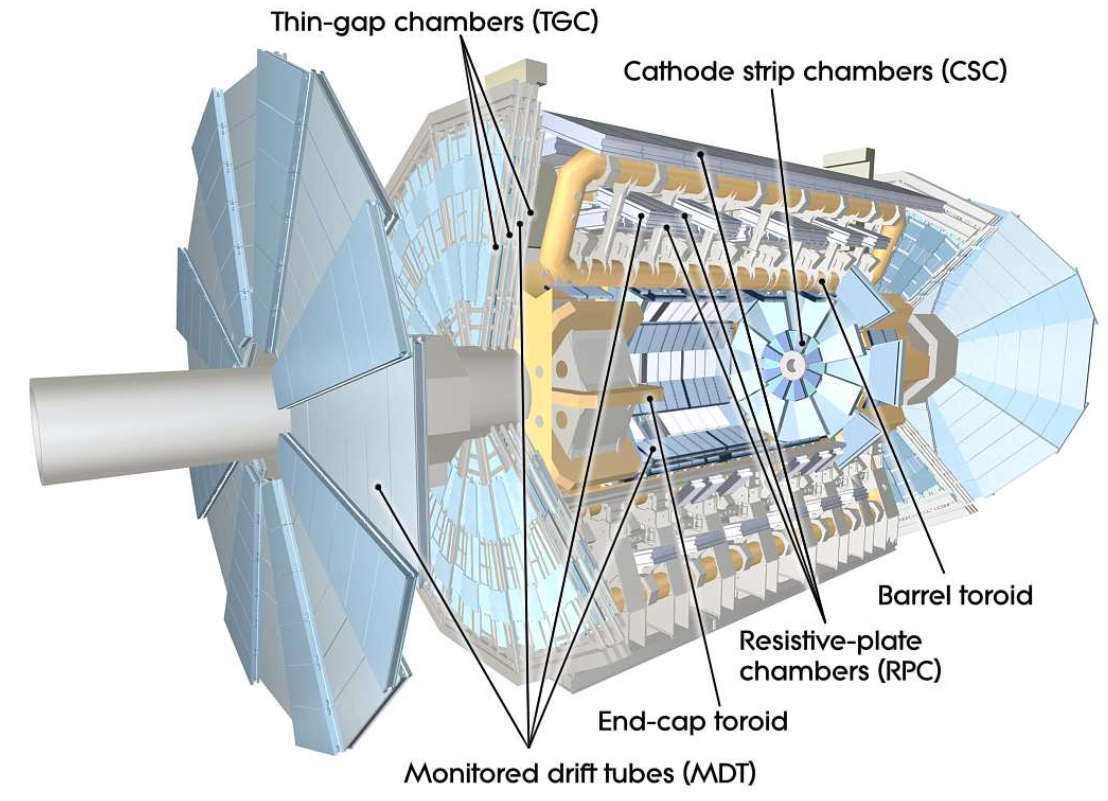
\includegraphics[width=.6\textwidth]{Detector_plots/Muon.png}
		\caption{Cut-away view of the ATLAS muon spectrometer system.}
		\label{fig:MS}
		\end{centering}
	\end{figure}
	
	
	The muon spectrometer (MS)~\cite{ATLAS-TDR-11} is the 
	outermost and largest detector of ATLAS. 
	The cut-away view of the MS is illustrated in Figure~\ref{fig:MS}.
	It fully covers the	calorimeter system and occupies a large part of the ATLAS cavern. 
	It is based on the magnetic deflection of muon tracks in the 
	large superconducting air-core toroid magnets, instrumented with
	separate trigger and high-precision tracking chambers. 
	Over the range $|\eta|< 1.4$, magnetic bending is provided by the large 
	barrel toroid. For $1.6 < |\eta|< 2.7$, muon tracks are bent by two smaller
	end-cap magnets inserted into both ends of the barrel toroid. 
	Over $1.4 < |\eta|< 1.6$, usually referred to as the transition region, 
	magnetic deflection is provided by a combination of barrel and end-cap
	fields. The configuration of magnets provides a field mostly orthogonal 
	to the muon trajectories, hence minimising the degradation of 
	resolution due to multiple scattering. 
	% The anticipated high level of 
	% particle flux has had a major impact on the choice and design of the spectrometer 
	% instrumentation, affecting performance parameters such as rate capability, granularity, ageing
	% properties, and radiation hardness.
	% In the barrel region, tracks are measured in chambers arranged in three cylindrical layers
	% around the beam axis; in the transition and end-cap regions, the chambers are installed in planes
	% perpendicular to the beam, also in three layers.


	The MS measures momentum of muons tracks depends on the momentum 
	of the tracks. 
	The resolution is typically 2–3\% over most of the kinematic range
	apart from very high momenta, where it increases to about 10\% at \pt\ = 1 TeV.  
	The MS consists of four subsystems which rely on four different gas detector
	technologies. Two of them, the resistive plate chambers (RPC) in the barrel region 
	and the thin gap chambers (TGC) in the end-cap region, provide trigger signals, 
	while the other two, the monitored drift tubes (MDT) and the cathode strip 
	chambers (CSC) provide the momentum measurement. The MDT chambers provide high 
	precision measurements in the bending direction over most of the detector
	acceptance while the CSC are used in the forward region where the particle flux 
	is too high for the MDT	chambers. The muon chambers are arranged in the barrel 
	($|\eta| < 1.05$) in three cylindrical layers around the beam axis, 
	while in the end-cap regions ($1.05 < |\eta| < 2.7$) they are placed in three wheels.

	\subsubsection{Trigger system}
	\begin{figure}[bht]
		\begin{centering}	
		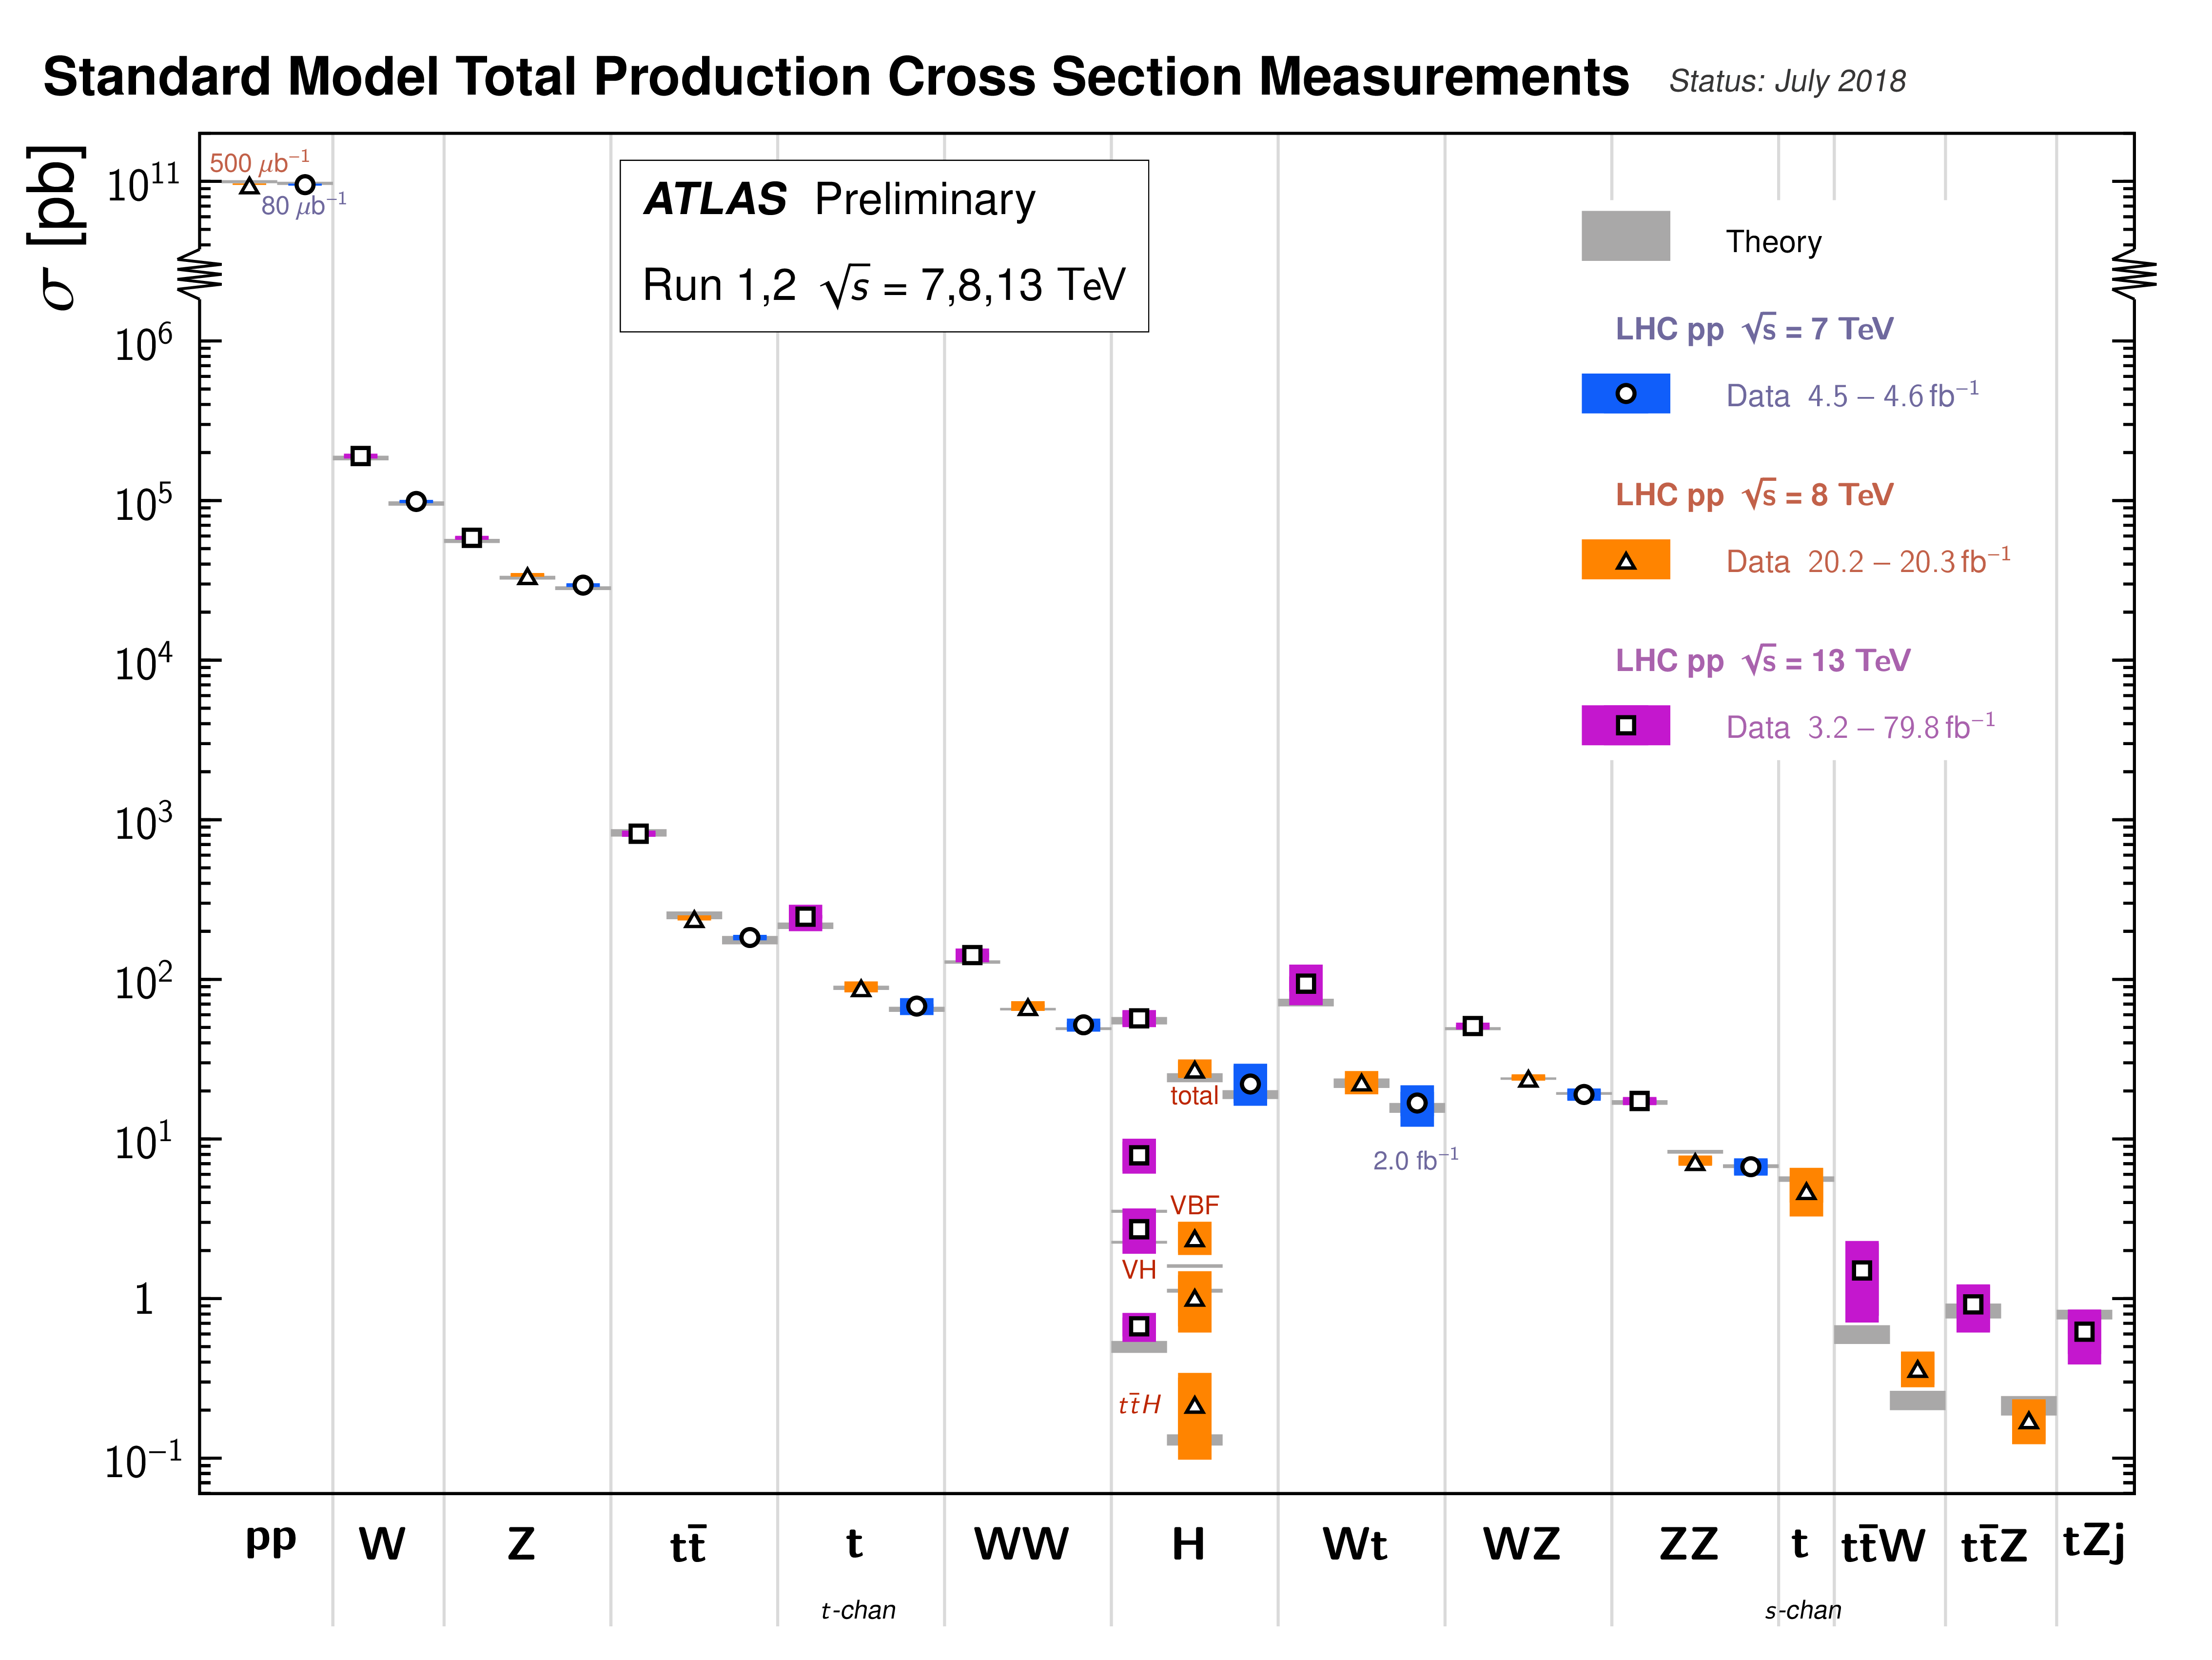
\includegraphics[width=.97\textwidth]{Detector_plots/summary xs.png}
		\caption{Plot showing the production cross-sections of the most dominant
		background processes at the LHC.}
		\label{fig:summary production Xs}
		\end{centering}
	\end{figure}
	As mentioned in section \ref{sec:runs and results}, the spacing of each bunch
	is 25 ns. This translates to a frequency of 40 MHz of bunch crossing. It
	will be difficult and not meaningful to keep all these events, which includes
	a lot of ``uninteresting'' physics events. Figure~\ref{fig:summary production Xs} 
	shows a summary of the most dominant background processes production cross-sections.
	Many of these processes produce high multiplicity of jets and are not of experimental
	interest. Therefore, it's necessary to adopts a trigger system that make fast decisions
	whether to save the event or not.
	The ATLAS trigger system consists of two consecutive parts: the Level 1 trigger
	\cite{ATLAS-TDR-12}, followed by the Level 2 and the event filter, 
	which together form the High Level Trigger (HLT)
	\cite{ATLAS-TDR-16}.
	
	The L1 trigger searches for signatures from high-\pt\ muons, electrons/photons, jets, and 
	\mbox{$\tau$-leptons} decaying into hadrons. It also selects events with large MET
	and large total transverse energy. The L1 trigger uses reduced-granularity information from a
	subset of detectors: the RPC and TGC for high-\pt\ muons, and all the calorimeter 
	sub-systems for electromagnetic clusters, jets, $\tau$-leptons, $E_{miss}^T$ ,
	and large total transverse energy.
	As a result, the L1 trigger reduces the event rate from 40 MHz to a maximum of 100 kHz.
	The decision is made by Central Trigger	Processor (CTP), 
	which operates on signals from dedicated hardware in the calorimeter
	and muon detector systems. The decision time, at under 2.5 $\mu s$, is faster than the ID
	can process events so ID information is omitted.
	For each data-taking period, the L1	trigger is loaded with a trigger menu, 
	a list of up to 256 criteria used to determine
	whether an event is accepted. The trigger menus are designed to accomodate a broad
	physics programme, with high acceptance for both BSM searches and SM precision
	measurements.

	The L1 trigger also uses detector information with reduced granularity to identify Regions
	of Interest (RoI)~\cite{Blair:2007qn} in $\phi$ and $\eta$.
	The L2 selection is seeded by the RoI information provided by the L1 trigger over a dedicated
	data path. L2 selections use, at full granularity and precision, all the available detector 
	data within the RoI’s.
	The L2 menus are designed to reduce the
	trigger rate to approximately 3.5 kHz, with an event processing time of about 40 ms,
	averaged over all events. The final stage of the event selection is carried out by 
	the event filter, which reduces the event rate to roughly 200 Hz. 
	The selections are implemented using offline analysis procedures
	within an average event processing time of the order of four seconds.
	



\chapter{Data and Monte Carlo samples}
\large
\chapter{Physics Objects Reconstruction}
\large
Particles produced in the $pp$ collisions inside ATLAS can interact with the detector subsystems
with each type of particle leaving a unique signature.
Reconstructing and identifying these particles precisely and efficienctly 
using the information recorded in each sub-detectors is a building stone of physics analysis.
Therefore, the following chapter outlines the reconstruction procedure of 
the particles important for the analysis present in this thesis, referred to
as `physics objects reconstruction'.
\section{Track and vertex reconstruction}
\label{sec:track}
Track and vertex reconstruction is a starting point of physics objects reconstruction, 
which makes it crucial to understand how they are implemented in ATLAS.
Track reconstruction~\cite{ATLAS-CONF-2012-042,PERF-2015-08} is done 
mainly with the ``inside-outside'' procedure, complemented by the ``outside-in'' 
and the reconstructing of TRT-standalone tracks. 
% As shown in Figure~\ref{fig:electron_recon}, a charged particle traverses
% the ID. Space points are formed using the ID information.
The inside-out stage starts from assembling the raw measurements
into \textit{clusters}:
an algorithm called connected component analysis~\cite{CCA} 
groups pixels and strips in a given sensor, 
where the deposited energy yields a charge above threshold, 
with a common edge or corner into clusters. 
% It is useful to introduce the several classes of clusters identified 
% by either the ``truth information'' (TODO: remove if this is mentioned earlier in the simulation), 
% only available in simulation and referring to information at MC generator level, 
% or reconstructed quantities in both collision data and MC simulation. 
% Clusters created by charge deposits from one particle
% are called \textit{single-particle} clusters, and clusters created by charge
% deposits from multiple particles are called \textit{merged} clusters.
% These definitions rely on truth information and both cases
% are illustrated in Figure \ref{fig:cluster}. 
% In addition, clusters that are used in multiple reconstructed tracks 
% but are not sufficiently compatible with the properties of a merged cluster
% to be identified as merged by the reconstruction are called \textit{shared} clusters.
%  \begin{figure}[bth]
%     \centering
%     \begin{subfigure}[t]{.38\linewidth}
%         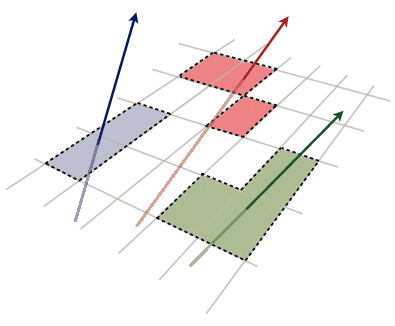
\includegraphics[width=1\textwidth]{Reconstruction_plots/single_cluster.png}
%         \caption{(a)}
%     \end{subfigure}
%     \begin{subfigure}[t]{.38\linewidth}
%         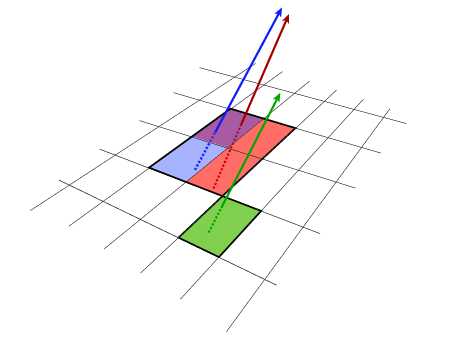
\includegraphics[width=1\textwidth]{Reconstruction_plots/merged_cluster.png}
%         \caption{(b)}
%     \end{subfigure}
    
%     \caption{Illustration of (a) single-particle pixel clusters on a pixel sensor and (b) 
%     a merged pixel cluster due to very collimated charged particles. 
%     Different colours represent energy deposits from different charged particles 
%     traversing the sensor and the particles trajectories are shown as arrows. 
%     Image taken from \cite{PERF-2015-08}.}
%     \label{fig:cluster}
% \end{figure}
From clusters, three-dimensional measurements referred to as
\textit{space points} are created (the yellow points in Figure~\ref{fig:track_recon}). 
They represent the point where the charged particle 
traversed the active material of the ID. 
Each space point equates to one cluster in the pixel detector, while in the SCT, 
clusters from both sides of a strip layer must be combined to obtain a three-dimensional measurement.
Three sets of space points are combined to track seeds 
(circled in blue in Figure~\ref{fig:track_recon}). 
% This approach maximizes the possible number of combinations while still allowing 
% a first crude momentum estimate. 
% The impact parameters of a track seed, 
% with respect to the centre of the interaction region, are estimated by assuming 
% a perfect helical trajectory in a uniform magnetic field.
A combinatorial Kalman filter~\cite{FRUHWIRTH1987444} is used to 
build track candidates from the chosen seeds by incorporating additional 
space points from the remaining layers of the pixel and SCT detectors which 
are compatible with the preliminary trajectory 
(circled in blue dashed line in Figure~\ref{fig:track_recon} ). 
\begin{figure}[bht]
    \begin{centering}	
    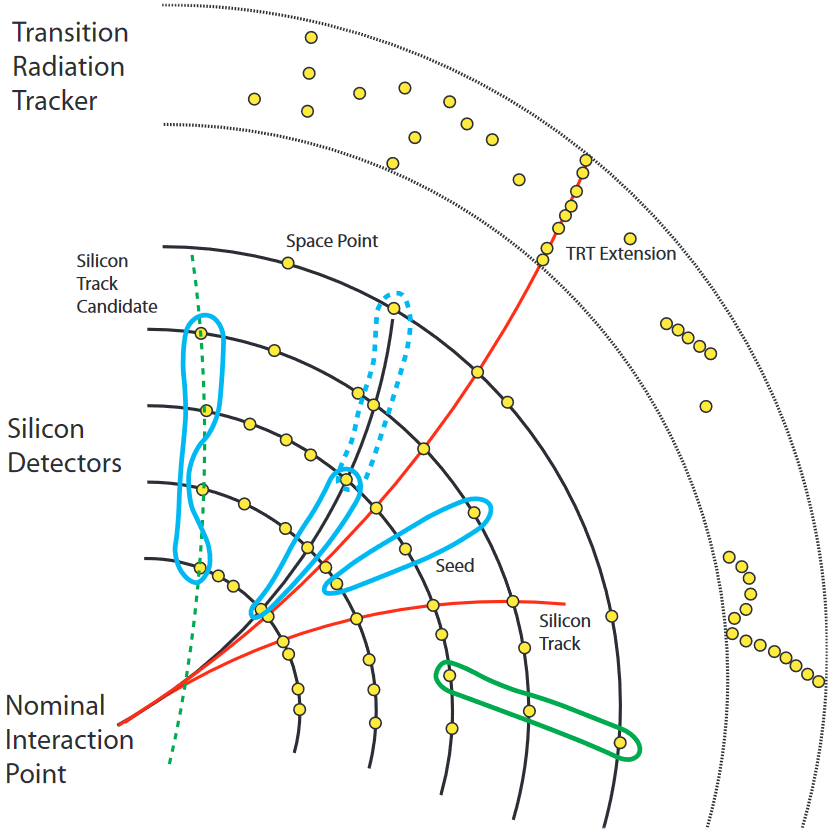
\includegraphics[width=.8\textwidth]{Reconstruction_plots/track.png}
    \caption{An example of track reconstruction. Image reproduced from~\cite{ATLAS-CONF-2010-072}.
        }
    \label{fig:track_recon}
    \end{centering}
\end{figure}
A track score computed by the quantities of the fitted track
is assigned to each track.
% including the $\chi^2$ of the fitting, intrinsic resolution, 
% expected clusters multiplicity, number of holes (missing hits) 
% and \pt. 
The tracks candidates are processed in descending order of 
track score,
those fail a set of minimum requirement on \pt, number of holes, 
number of clusters etc are rejected;
candidates that have too many bad quality clusters are 
stripped down and re-scored and returned to the list
of remaining candidates.
This process is referred to as ``ambiguity solving''~\cite{PERF-2015-08}.
%  track candidates are fitted if they fulfil 
% a set of minimum requirement 
% on \pt\, number of holes, number of clusters etc.
% After that, the fitted tracks with too many shared clusters 
% (with additional artificial neural network to identify these shared clusters)  
% are striped down and re-scored, 
% and returned to the ordered list of remaining candidates;
% the fitted tracks with too many holes or too few clusters are rejected;
% those pass through the above requirement are accpeted and added 
% to the final track collection. 
% This process is referred to as ``ambiguity solving''~\cite{PERF-2015-08}.
Finally, the tracks are extended into the TRT, and by using the full information
of the three sub-detectors, the tracks are fitted again to estimate the final track
impact parameter (IP, transverse distance from the interaction point) $d_0$, 
distance from the interaction point along the $z$ axis $z_0$,
azimuthal angle $\phi$, polar angle $\theta$ and charge momentum ratio $q/p_T$.

The complementary ``outside-in'' algorithm starts with searching for tracks with segments 
reconstructed in the TRT, and extend the tracks inwards by adding silicon hits.
The tracks are built with the combinatorial Kalman filter and passed to the
ambiguity solving procedure.
% Back-tracking is designed to reconstruct tracks of secondary particles, which are
% produced in the interactions of primary particles.
Finally, tracks with a TRT segment but no extension into the silicon detectors
are referred as TRT-standalone tracks. 

After the tracks are reconstructed, primary vertices,
which are the points where the hard scattering occured,
is reconstructed in two steps~\cite{ATLAS-CONF-2010-069}:
a) the primary vertex finding algorithm, 
dedicated to associate reconstructed tracks to the vertex candidates, 
and b) the vertex fitting algorithm, 
dedicated to reconstruct the vertex position. 
Vertex seeds are obtained from the $z$-position at the beamline of the reconstructed tracks. 
An iterative $\chi^2$ fit is made using the seed and nearby tracks. 
Each track carries a weight which is a measure of its compatibility 
with the fitted vertex depending on the $\chi^2$ of the fit. 
Vertices are required to contain at least two tracks, and 
tracks displaced by more than 7$\sigma$ from the vertex are used to
seed a new vertex and the procedure is repeated until no additional vertices can be found. 
This procedure is repeated until no unassociated tracks are left in the event or no
additional vertex can be found. 
The primary vertex for each event is selected as the vertex with the highest
$\sum_{tracks}(p_T^{track})^2$.



\large
\section{Electron}
\label{sec:electron}
When an high energy electron (or positron) enters the detector, 
it interacts with the detector material primarily via bremsstrahlung. 
This results in radiation of photons, which subsequently convert into 
electron–positron pairs which continue to 
interact with the detector material, 
leading to a cascade of particles of decreasing energy.
These cascade particles are usually referred to as electromagnetic \textit{shower}.
They are very collimated and frequently create neighbouring signals in the calorimeter component. 
% as part of the same electromagnetic cluster. 
These interactions can occur inside the inner-detector volume 
or even in the beam pipe, generating multiple tracks
in the inner detector, or can instead occur downstream 
of the inner detector, only impacting the shower in
the calorimeter. 
\subsection{Reconstruction}
% Therefore, it is possible to produce and match multiple tracks to the same electromagnetic
% cluster, all originating from the same primary electron.
The reconstruction of electron is based on three fundamental components: 
a) localised clusters of energy deposits found within the EM calorimeter, 
b) charged tracks identified in the ID (as described in details in chapter~\ref{sec:track}),
and c) close matching in $\eta \times \phi$ space of the tracks to the clusters~\cite{PERF-2017-01}.
Figure~\ref{fig:electron_recon} provides a schematic illustration of the elements that enter into
the reconstruction and identification of an electron. 
\begin{figure}[bht]
    \begin{centering}	
    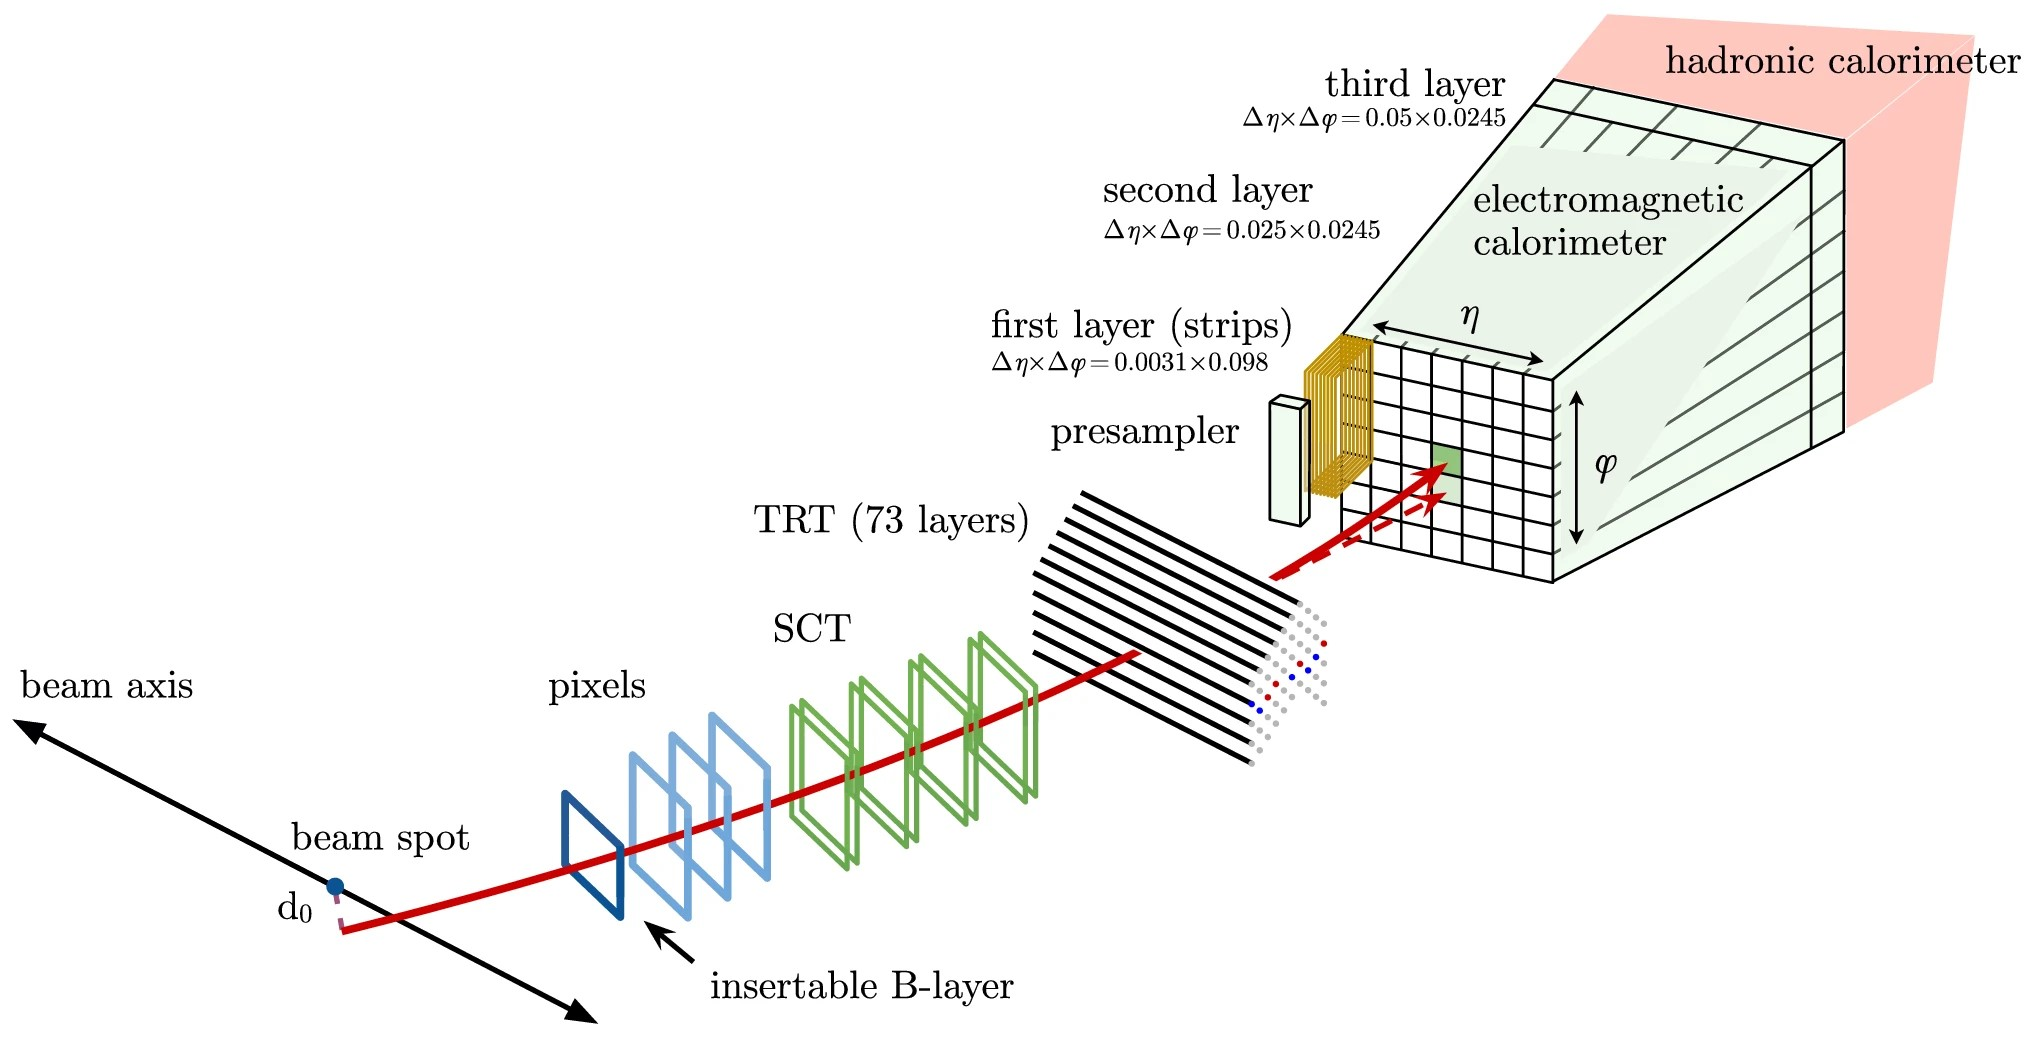
\includegraphics[width=1.0\textwidth]{Reconstruction_plots/electron.jpg}
    \caption{A schematic illustration of the path of an electron through the detector. 
    The red trajectory shows the 
    hypothetical path of an electron, which first traverses the tracking system (pixel detectors, then SCT
    and lastly the TRT) and then enters the electromagnetic calorimeter. 
    The dashed red trajectory indicates the path of a
    photon produced by the interaction of the electron with the material in the tracking system. 
    Image taken from~\cite{PERF-2017-01}.
        }
    \label{fig:electron_recon}
    \end{centering}
\end{figure}
The reconstruction starts from EM cluster seeding from localised energy deposits 
using a sliding-window algorithm~\cite{sliding-window}.
The $\eta \times \phi$ space of the EM is divided into \textit{towers} of 200 $\times$ 256
elements of size $\Delta\eta \times \Delta\phi$ = 0.025 $\times$ 0.025, 
consistent with the granularity of the second layer of the EM calorimeter. 
Then algorithm then ``slides'' a rectangular window of size 3 $\times$ 5 towers 
whose summed transverse energy exceeds 2.5 GeV to form a seed-cluster.
The centre of the seed moves in steps of 0.025 in either $\eta$ or $\phi$ direction 
to search for localised energy deposits; 
this process is repeated until every element of the calorimeter has been covered.
To better account for the energy loss of charged particles in material,
a subsequentl fitting procedure using optimised Gaussian-sum filter \cite{ATLAS-CONF-2012-047} 
is performed on tracks which are ``loosely'' matched to the EM clusters, 
which requires the tracks and clusters to satisfy:
$|\eta_{cluster} - \eta_{track}|$ < 0.05
and one of the two requirements:
$-0.20 < \Delta \phi < 0.05$ 
or
$-0.10 < \Delta \phi_{res} < 0.05$,
where $\Delta\phi \equiv -q \times (\phi_{cluster} - \phi_{track})$ with 
$q$ being the charge of the particle, and 
$\phi_{cluster}$, $\phi_{track}$ and $\eta_{cluster}$, $\eta_{track}$ 
are the $\phi$, $\eta$ coordinates of
the cluster barycentre and the poisition of the track extrapolated from the 
perigee to the second layer of the calorimeter, respectively;
$\Delta \phi_{res}$ is similar to $\Delta \phi$ but with the 
momentum of the track rescaled to the energy of the cluster.
The assymmetry in the condition is to account for the energy loss
due to bremsstrahlung where tracks with negative (positive) electric charge
bend due to the magnetic field in the positive (negative) $\phi$ direction.

The matching of the fitted tracks to the candidate calorimeter seed-cluster
is the final step of electron reconstruction. 
The matching requires $-0.10 < \Delta\phi < 0.05$,
with the other alternative requirement remaining the same.
If several tracks fulfil the matching criteria, 
the track considered to be the primary electron track is selected 
using an algorithm that takes into account the distance in $\eta$
and $\phi$ between the extrapolated tracks and the cluster barycentres 
(agian, measured in the second layer of the calorimeter), 
the number of hits in the silicon detectors and in the innermost silicon layer; 
a candidate with an associated track with at least four hits in the silicon layers and no association
with a vertex from a photon conversion is considered as an electron candidate. 
However, if the primary candidate track can be matched to a secondary vertex and has no pixel hits, 
then this object is classified as a photon candidate (likely a conversion). 

A further classification is performed using the candidate electron’s $E/p$ and \pt, 
the presence of a pixel hit, and the secondary-vertex information, to determine
unambiguously whether the object is only to be considered as an electron candidate or if it should be
ambiguously classified as potentially either a photon candidate or an electron candidate.

\subsection{Identification} 
The reconstruction algorithm is very efficient in reconstructing electron,
however, this is not necessarily what is needed for many ATLAS analysis, where
they are insterested in prompt electrons. 
Prompt electrons are electrons coming from the collision of the an event, 
while non-prompt electrons may come from
the semileptonic decays of heavy quarks or from photon conversion.
Other objects such as hadrons can be mis-reconstructed as electron as well.
It necessitates the identification of prompt electrons, making use of the 
differences between prompt electrons and non-prompt electrons/mis-reconstructed electrons.
A multivariate likelihood technique, taking advantages of the correlations
among the variables describing the differences,
is employed to select prompt electrons~\cite{PERF-2017-01}.
The input to the likelihood includes the differences of: 
a) shower shape, b) properties of the track, c) matching
of the track and clusters.
In addition, many analysis further require the electron to pass
some \textit{isolation} requirements.
Isolation is built exploiting a characteristic signature 
of the prompt electrons that 
there is relatively little activity surrounding 
the prompt electrons, as compared to non-prompt electrons~\cite{EGAM-2018-01}. 

To quantify the performance of the identification, 
the identification efficiency is measure, which represents the probability of
a prompt electron being reconstructed as an electron.
Different cuts are applied on the final discriminant
to define \textit{working points} (WP), which can specify 
the identification efficiency, as a function of $E_T$ or $\eta$ of the electron. 
Three WPs, \textit{Loose}, \textit{Medium} and \textit{Tight} are defined, 
each WP places a different requirement on final discriminant 
made with a different set of variables. 
An example of the electron identification efficiency 
is shown in Figure~\ref{fig:electron_ID}.
\begin{figure}[bht]
    \begin{centering}	
    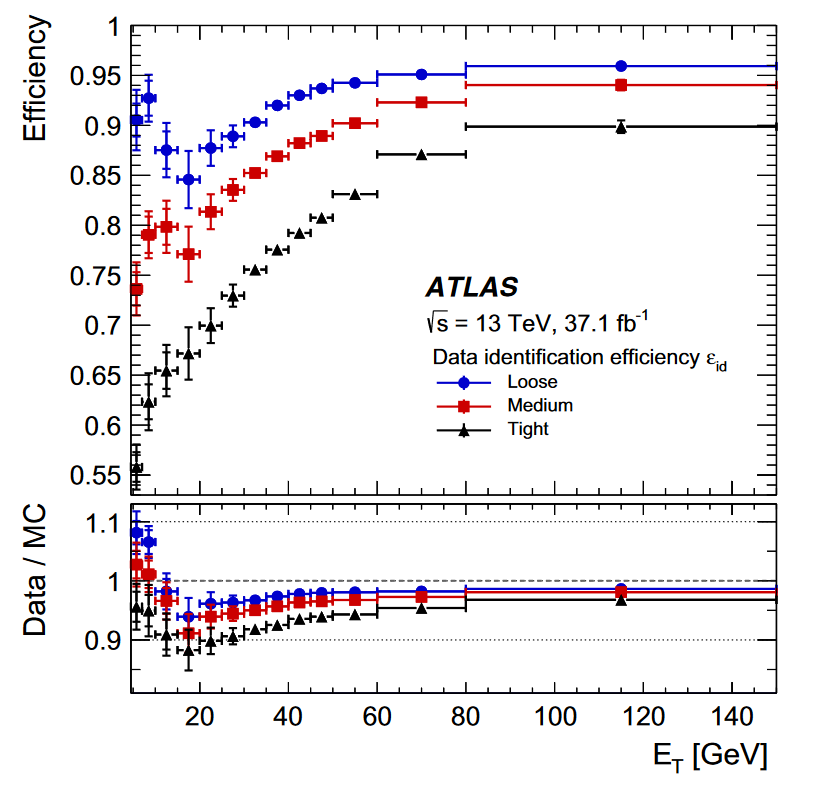
\includegraphics[width=0.45\textwidth]{Reconstruction_plots/electrond_ID1.png}
    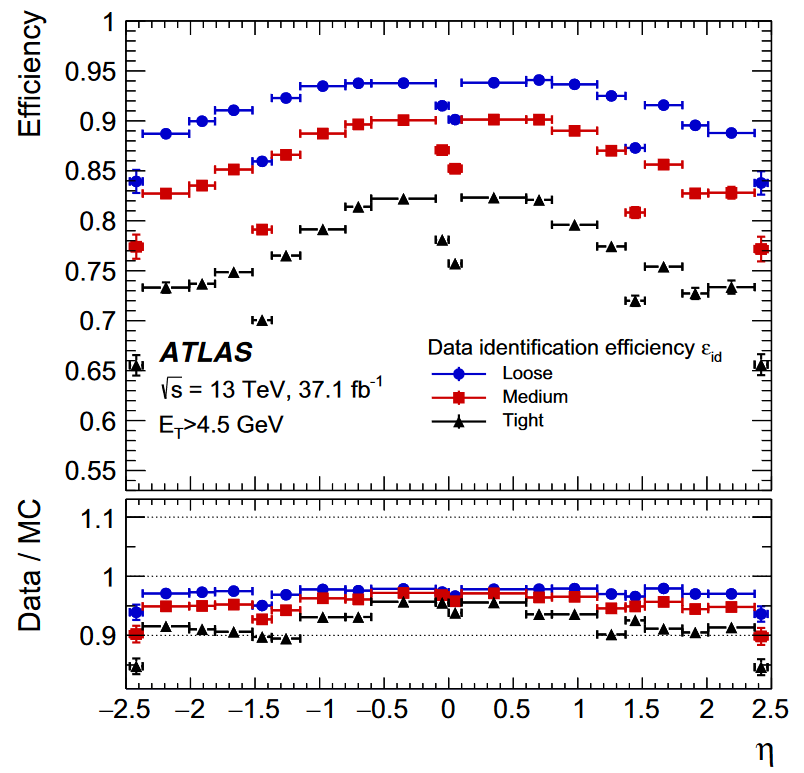
\includegraphics[width=0.45\textwidth]{Reconstruction_plots/electrond_ID2.png}
    \caption{Measured electron identification efficiencies in $Z \rightarrow ee$
    events for the `Loose' (blue circle), `Medium' (red square), 
    and `Tight' (black triangle) WPs as a function of $E_T$ (left) and $\eta$ (right). 
    The vertical uncertainty bars (barely visible because they are small) 
    represent the statistical (inner bars) and total (outer bars) uncertainties. 
    For both plots, the bottom panel shows the data-to-simulation
    ratios. Reproduced from Reference~\cite{PERF-2017-01}.}
    \label{fig:electron_ID}
    \end{centering}
\end{figure}
Similary for electron isolation, 
four WPs: \textit{Gradient}, \textit{HighPtCaloOnly}, \textit{Loose} and \textit{Tight} 
are defined, each targeting a fixed value of isolation efficiency
or imposing fixed requirement on the isolation variables. 

In the analysis presented in Chapter~\ref{sec:search for dihiggs} 
the `Loose' identification WP is used, 
with additional requirements on the electron \pt\ > 7 GeV and $|\eta|$ < 2.47;
the electron candidates are also required
to pass the ‘Loose’ isolation WP which has an efficiency of 99\%. 
The isolation requirement is also 
inverted to provide control regions for estimating backgrounds.
% , achieving 99\% efficiency 
% that is constant across the entire \pt\ spectrum.
In the calibration effort presented in Chapter~\ref{sec:FTAG} 
the `Medium' identification WP is used, 
with additional requirements on the electron \pt\ > 27 GeV and $|\eta|$ < 2.47;
electrons are required to pass the `Gradient' isolation WP,
designed to give an efficiency of 90\% at \pt\ = 25 GeV and 99\% at \pt\ = 60 GeV.
The different requirements in the two chapters 
is the result of different signal targeted and hence different 
purity and phase space is needed. 
% The `Loose' WP features variables most useful for discrimination against light-flavour jets. 
% In the `Medium' and `Tight' regimes, additional variables are added for further rejection 
% of heavy-flavour jets and photon conversions. 
% Although different variables are used for the different selections, a sample of electrons selected using a tighter LH
% is a subset of the electron samples selected using the looser LH to a very good approximation

% \textit{isolation} is built, usually by 
% summing the transverse energies of clusters in the calorimeter 
% or the transverse momenta of tracks in a cone of radius
% $\Delta R$ around the direction of the electron
% candidate, excluding the candidate itself

% The inputs to the likelihood include measurements from the tracking system, the
% calorimeter system, and quantities that combine both tracking and calorimeter information.
% The main advantages using the likelihood-based method comparing with 
% a selection-criteria-based (so-called ``cut-based'') identification is that
% a prompt electron may fail the cut-based identification because it
% does not satisfy the selection criterion for a single quantity, 
% while in the likelihood-based selection this electron can
% still satisfy the identification criteria, 
% because the likelihood combines the information of all of the discriminating variables.
% The final discriminant produced by the likelihood method is used to define 
% three \textit{working points} (WP), which are cuts in the final discriminant 
% identifying the different identification efficiencies. 






\section{Muon}
\subsection{Reconstruction}
The characteristic behaviour of a muon in the detector is a particle
ionising minimally. 
The muon reconstruction is done taking advantage of this feature, 
with information from the ID and MS tracking detectors, while
information from the calorimeters is also used
for determination of track parameters and to account for cases of
large energy loss in the calorimeters, and for MS-independent
tagging of ID tracks as muon candidates~\cite{CERN-EP-2020-199}.
The muon reconstruction consists of two steps. 
The first step is to reconstruct the stand-alone track in the MS,
followed by reconstruction with complete detector information.

The first step of reconstruction starts with the identification 
of short straight-line local track segments reconstructed 
from hits in an individual MS \textit{stations} (layers). 
These segments are then combined into preliminary track candidates, 
with information from precision measurements in the bending plane 
and measurements of the second coordinate from 
the MS triggers to create three-dimensional track candidates. 
A global $\chi^2$ fit of the muon trajectory 
through the magnetic field is performed,
outlier hits are removed and hits along the trajectory that
were not assigned to the original track candidate are added.
Finally, the tracks are fitted again with the updated hits information,
and ambiguities are resolved by removing tracks
that share a large fraction of hits with higher-quality tracks.

The second step of reconstruction is to combine the track candidates 
with the complete information of all sub-detectors.
The reconstruction proceeds according to five main
reconstruction strategies, leading to the corresponding muon
types: 
\begin{itemize}
\item \textit{combined muons} 
are identified by matching 
MS tracks to ID tracks and performing a combined track fit 
based on the ID and MS hits, taking into account the energy loss in the
calorimeters.
\item \textit{Inside out muons} 
are reconstructed using a complementary
inside-out algorithm, which extrapolates ID tracks to the MS
and searches for at least three loosely-aligned MS hits. The
ID track, the energy loss in the calorimeters and the MS hits
are then used in a combined track fit. 
% This algorithm does
% not rely on an independently reconstructed MS track, and
% therefore recovers some efficiency.
\item \textit{Muon-spectrometer extrapolated muons} are muons 
when an MS track cannot be matched to an ID track. Its parameters 
are extrapolated to the beamline and used to define an
Muon-spectrometer extrapolated muon. 
Such muons are used to extend the acceptance
outside that of the ID, thus fully exploiting the full MS 
coverage up to $|\eta|$ = 2.7.
\item \textit{segment-tagged muons} 
are identified by requiring that an ID track
extrapolated to the MS satisfies tight angular matching
requirements to at least one reconstructed MS segment. 
% A successfully-matched ID track is identified as a muon candidate, 
% and the muon parameters are taken directly from the
% ID track fit.
\item \textit{calorimeter-tagged muons} 
are identified by extrapolating ID
tracks through the calorimeters to search for energy deposits
consistent with a minimum-ionising particle.
\end{itemize}
\subsection{Identification}
Muon identification is performed by applying quality requirements that suppress background, 
mainly from pion and kaon decays, while selecting prompt muons with high efficiency.
Muon candidates originating from in-flight decays of charged hadrons in the ID 
are often characterized by the presence of a distinctive “kink” topology 
in the reconstructed track. 
As a consequence, it is expected that the fit quality of the resulting combined track 
will be poor and that the momentum measured in the ID and MS may not be compatible~\cite{PERF-2015-10}. 
Therefore, a set of requirements on the
number of hits in the different ID subdetectors and different
MS stations, on the track fit properties, 
and on variables that test the compatibility of the individual measurements 
in the two detector systems~\cite{CERN-EP-2020-199}.
A set of WPs are defined for each of the munon types defined in the 
previous section. 
The main metrics considered for designing the WPs are 
the selection efficiency and purity in simulation,
where the prompt muon efficiency of a selection WP 
represents the probability that a prompt muon traversing the detector 
is reconstructed as a muon and satisfies the WP; the purity
of a selection WP is one minus the hadron misidentification
rate (the fraction of light hadrons reconstructed as muons 
and satisfying the WP).
Three standard selection WPs: \textit{Loose},
\textit{Medium}, and \textit{Tight} are designed to 
cover the majority of physics analysis, with 
two additional WPs, \textit{High-\pt} and \textit{Low-\pt}
are designed to accommodate the analysis targeting extreme 
phase space. 
In Chapter~\ref{sec:search for dihiggs}, muons are selected
with \pt\ > 7 GeV and $|\eta|$ < 2.7, and passing the `loose' 
identification criteria as well as the `pflowLoose\_VarRadIso' 
isolation criteria~\cite{MuonWP};
while in Chapter~\ref{sec:FTAG} muons are selected
with \pt\ > 27 GeV and $|\eta|$ < 2.5, and passing the `medium' 
identification criteria as well as a track-based isolation criteria.
An example of the reconstruction and isolation efficiency of muon is 
shown in Figure~\ref{fig:muon_ID}.
\begin{figure}[bht]
    \begin{centering}	
    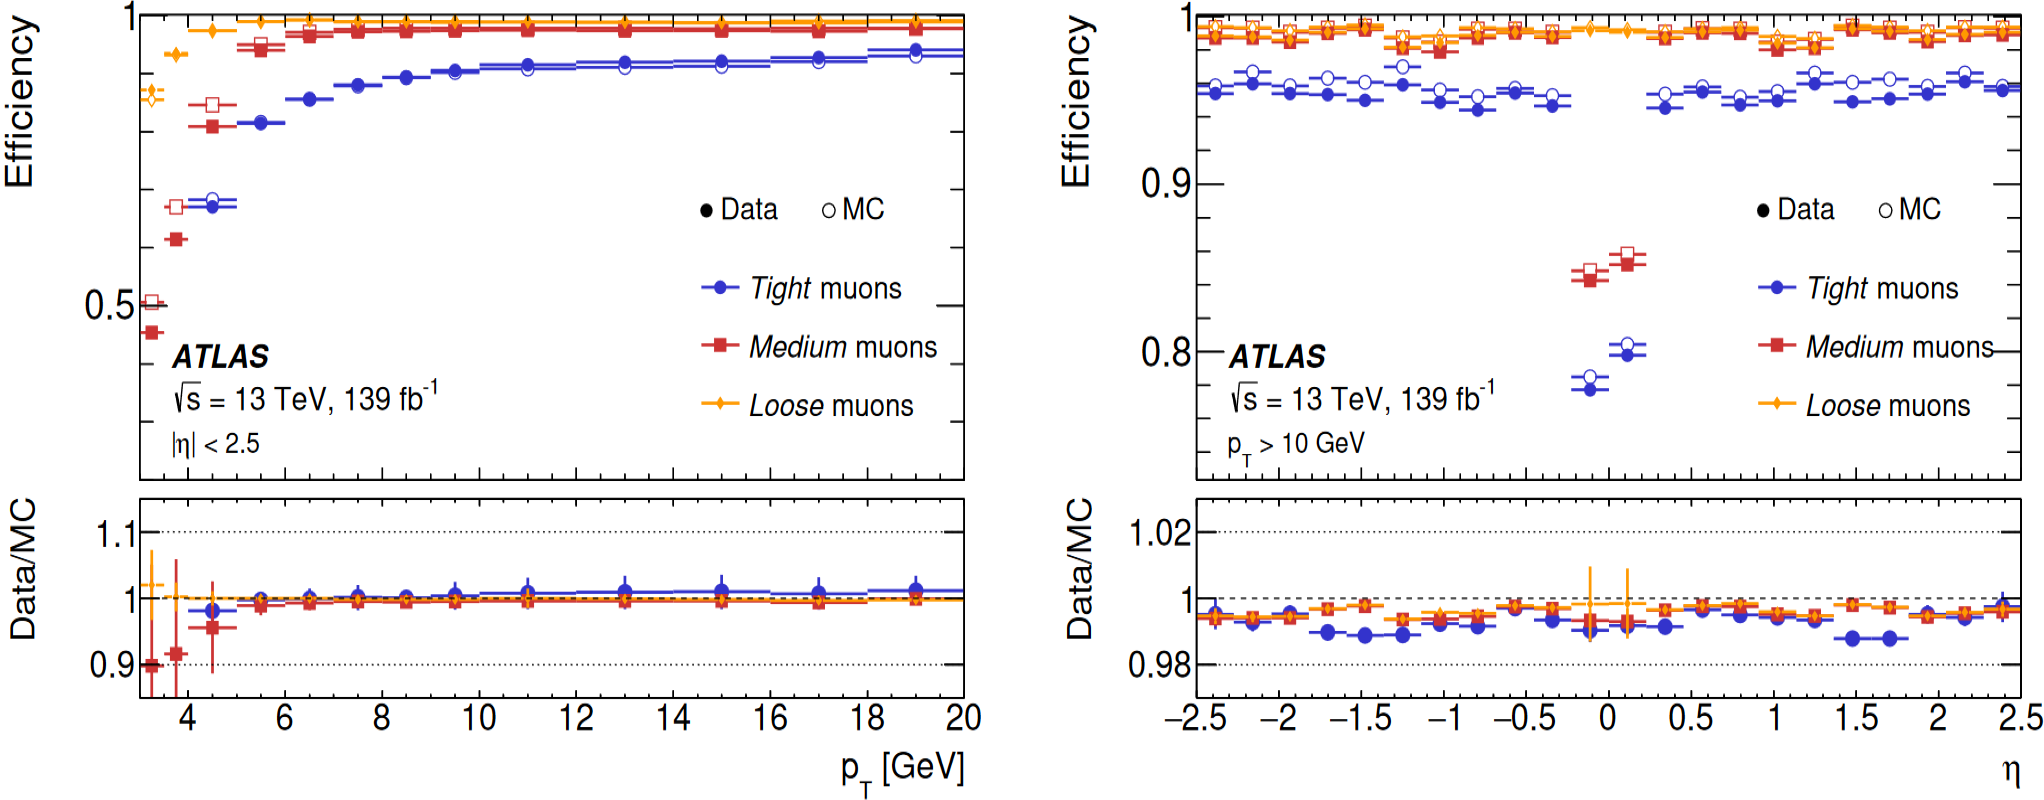
\includegraphics[width=1.0\textwidth]{Reconstruction_plots/muon_ID.png}
    \caption{
        Muon reconstruction and identification efficiencies for the Loose, Medium, and Tight criteria. 
        The left plot shows the efficiencies measured in $J/\psi \rightarrow \mu\mu$ events as function of \pt. 
        The right plot displays the efficiencies measured in $Z \rightarrow \mu\mu$ events as a function of $\eta$, 
        for muons with \pt\ > 10 GeV. The predicted efficiencies are depicted as open markers, 
        while filled markers illustrate the result of the measurement in collision data. 
        The statistical uncertainty in the efficiency measurement is smaller than the size of the markers, 
        and thus not displayed. The panel at the bottom shows the ratio of the measured to predicted efficiencies, 
        with statistical and systematic uncertainties.
    ratios. Reproduced from Reference~\cite{CERN-EP-2020-199}.}
    \label{fig:muon_ID}
    \end{centering}
\end{figure}

\section{Jet}
\label{sec:jet} 
\subsection{Reconstruction}
\large
A jet can be defined as a collimated spray 
of stable particles arising from the fragmentation
and hadronisation of a parton (quark or gluon) after a collision.
Jets provide a link between the observed colourless 
stable particles and the underlying physics at the partonic
level. A basic illustration of a collision of two protons,
the subsequent particle shower and a reconstructed jet is 
shown in Figure~\ref{fig:jets}.

\begin{figure}[bht]
    \begin{centering}	
    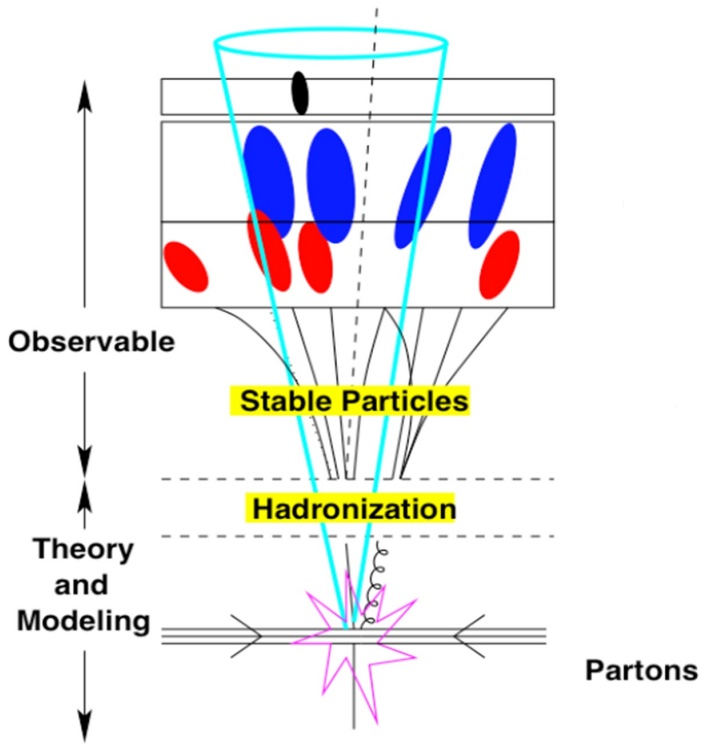
\includegraphics[width=.6\textwidth]{Reconstruction_plots/Jets.jpg}
    \caption{A simple example of an event showing the point of collision, 
    the fragmentation and hadronization of the quarks and gluons and the 
    resulting jet found through the detection of the stable particles. 
    Image reproduced from~\cite{atkin2015review}.
        }
    \label{fig:jets}
    \end{centering}
\end{figure}

The jet reconstruction starts by forming clusters of energy deposit
in the calorimeters performing a three-dimensional topological clustering 
of individual calorimeter cell signals~\cite{Aad_2017}.
The algorithm clusters the energy deposits into so called ``topo-clusters'' 
and combines their four-momenta. 
In Run 1 of the LHC, the ATLAS experiment used either
solely the calorimeter or solely the tracker to reconstruct
hadronic jets and soft particle activity, 
and the vast majority of analysis utilised jets that were built 
from topo-clusters, referred to \textit{EMTopo jets}.
% These jets were then calibrated to the particle level using a jet energy scale
% (JES) correction factor [4–7]. For the final Run 1 jet calibration, this correction factor also took into account the tracks
% associated with the jet, as this was found to greatly improve
% the jet resolution [4]. 
An alternative approach called ``\textit{Particle flow}'' (PFlow) was done
in ATLAS, as described in details in reference~\cite{PERF-2015-09}. 
It is the default approach for the thesis.
Measurements from both the tracker and the calorimeter 
are combined to form the signals. 
More specifically, the algorithm matches the reconstructed tracks
to the candidate leptons and hadrons, in oder to produce a new
set of clusters called \textit{PFlow clusters} from topo-clusters.
% The energy deposited in the calorimeter by all the charged particles is removed.
% Jet reconstruction is then performed on topo-clusters
% consisting of the remaining calorimeter energy and 
% tracks which are matched to the hard interaction.
% The main advantages of integrating tracking and calorimetric information 
% into one hadronic reconstruction step is that for 
% low-energy charged particles, the momentum resolution of the tracker is significantly
% better than the energy resolution of the calorimeter (see Table \ref{tab:ATLAS_performance}).
% Above $p_T^{track}$ = 100 GeV no track information is used as the PFlow algorithm 
% becomes equivalent to EMTopo benefitting from excellent
% calorimeter performance at high energies.
% In addition, with track reconstructed, one can ascertain whether it is 
% associated with a vertex. This information can be used to mitigate 
% in-time pileup signals. 
Using the PFlow clusters as inputs, PFlow jets are then reconstructed
using the anti-$k_t$ algorithm~\cite{Cacciari_2008}. 
% The inputs to jet reconstruction are 
% the tracks that are matched to the primary vertex,
% and positive energy topo-clusters which survives the energy subtraction step 
% and matches to the selected tracks. 
The anti-$k_t$ algorithm 
sequentially combines PFlow clusters into larger clusters based on the 
momentum-weighted distance between clusters. 
For two clusters $i$ and $j$ the algorithm defines:
\[  d_{i,j} = min(p_{T,i}^{2p},p_{T,j}^{2p}) \frac{\Delta R_{i,j}^2}{R^2} \]
and 
\[ d_{i,beam} = p_{T,i}^{2p} \]
where $p$ is a exponent parameter and the value of -1 is used
for the anti-$k_t$ algorithm (as the name `anti' suggests),
$\Delta R^2{i,j} = (\eta_i - \eta_j)^2 + (\phi_i - \phi_j)^2 $, 
and $p_{T,i}$, $\eta_i$ and $\phi_i$ are 
the transverse momentum, 
pseudorapidity and azimuthal coordinate
of cluster $i$, respectively. 
The parameter $R$ controls the size of the jet and for standard jets 
in ATLAS this is chosen to be $R$ = 0.4.
The algorithm combines objects $i$, $j$ with minimum value of $d_{i,j}$
into one object iterartively, until no more $d_{i,j}$ can be found greater
than $d_{i,beam}$, where the combined object is considered the final jet 
candidate.
% The algorithm calculates $d_{i,j}$ iterartively for all clusters: 
% when $d_{i,j} < d_{i,beam}$, the two clusters $i$, $j$ are combined
% into a single cluster, and the new cluster is added back to the list
% of consideration; when $d_{i,j} > d_{i,beam}$, the cluster $i$ is 
% considered final jet candidate and it is removed from the list of clusters.
% The anti-$k_t$ algorithm uses $p$ = -1 (as the name `anti' suggests), 
% which means that algorithm is more likely to combine two clusters with 
% very close to each other (as a result of the $\frac{\Delta R_{i,j}^2}{R^2}$ term)
% or cluster having large \pt\ with clusters having smaller \pt\ (as a result of
% the $min(p_{T,i}^{2p},p_{T,j}^{2p})$ term). 

A validation study is done by the author for comparison of the EMTopo jets 
to PFlow jets used in the analysis TODO: add reference after selection is defined.

\subsection{Calibration}
After the jets are reconstructed, the four-momenta of jets
are calibrated with the jet energy scale (JES) calibration
consists of several consecutive stages derived from a
combination of MC-based methods and in situ techniques \cite{PERF-2016-04}.
MC-based calibrations correct the reconstructed jet four momentum 
to that found from the simulated stable particles 
within the jet. 
The calibrations account for features of the
detector, the jet reconstruction algorithm, jet fragmentation,
and the busy data-taking environment resulting from multiple $pp$ 
interactions, and the difference in jet response between
data and MC simulation.
In order to calibrate jet energy resolution (JER),
jet momentum must be measured precisely. 
As described in details in reference \cite{JETM-2018-05},
a \textit{dijet balance} approach is used for this purpose with well-defined dijet system,
where the two jets are expected to have \pt\ that sum up to 0 precisely.
Furthermore, jets arised from pileup are suppressed by using the 
\textit{jet vertex tagger}, which is a multivariate 
combination of track-based variables developed to separate 
hard-scatter jets from pileup jets~\cite{ATLAS-CONF-2014-018}.
A jet cleaning selection is applied in order to veto any `fake' jets, 
which arise from non-collision background events, such as cosmic rays, 
or from detector effects. 
Finally, all jets in the analysis are required to have \pt\ < 20 GeV 
and $|\eta|$ < 2.5.


\subsection{Identification of heavy quark flavoured jets}
\label{sec:Flavour tagging}
As frequently being called \textit{flavour tagging}, 
the identification of jets containing $b$-hadrons (\bjets) 
against the large background of jets containing $c$-hadrons 
(\cjets) or jets coming from the hadronization of light ($u$,$d$,$s$) 
quarks or gluons (light jets) is of major importance in many areas of the 
physics programme of the ATLAS experiment at the LHC. 
It is crucial in a large number of SM
precision measurements, studies of the Higgs boson properties, 
searches for new phenomena~\cite{SUSY-2014-08, ATLAS-CONF-2018-043,Interpreting_Higgs_result},
and it also plays an important role in 
the $HH \to bb\tau\tau$ searches presenting in Chapter \ref{sec:search for dihiggs}. 

% as well as the recent 
% observation of the Higgs boson decay into bottom quarks~\cite{HIGG-2018-04} 
% and of its production in association with a top-quark pair~\cite{HIGG-2018-13}. 


The ATLAS Collaboration uses various algorithms to identify 
\bjets~\cite{PERF-2012-04}, referred to as \btagging\ algorithms, 
when analysing data recorded during Run 2 of the LHC. These 
algorithms exploit the long lifetime, high mass and high decay 
multiplicity of $b$-hadrons, as well as the properties of the \bquark\  
fragmentation. Given a lifetime of the order of 1.5 ps, $b$-hadrons have a 
significant mean flight length ($\langle c\tau \rangle$ $\approx$ 450 $\mu m$), 
in the detector before decaying, generally leading to at least one vertex 
displaced from the hard-scatter collision point, as illustrated in Figure~\ref{fig:b-jet-decay}.

\begin{figure}[bth]
	\begin{centering}	
	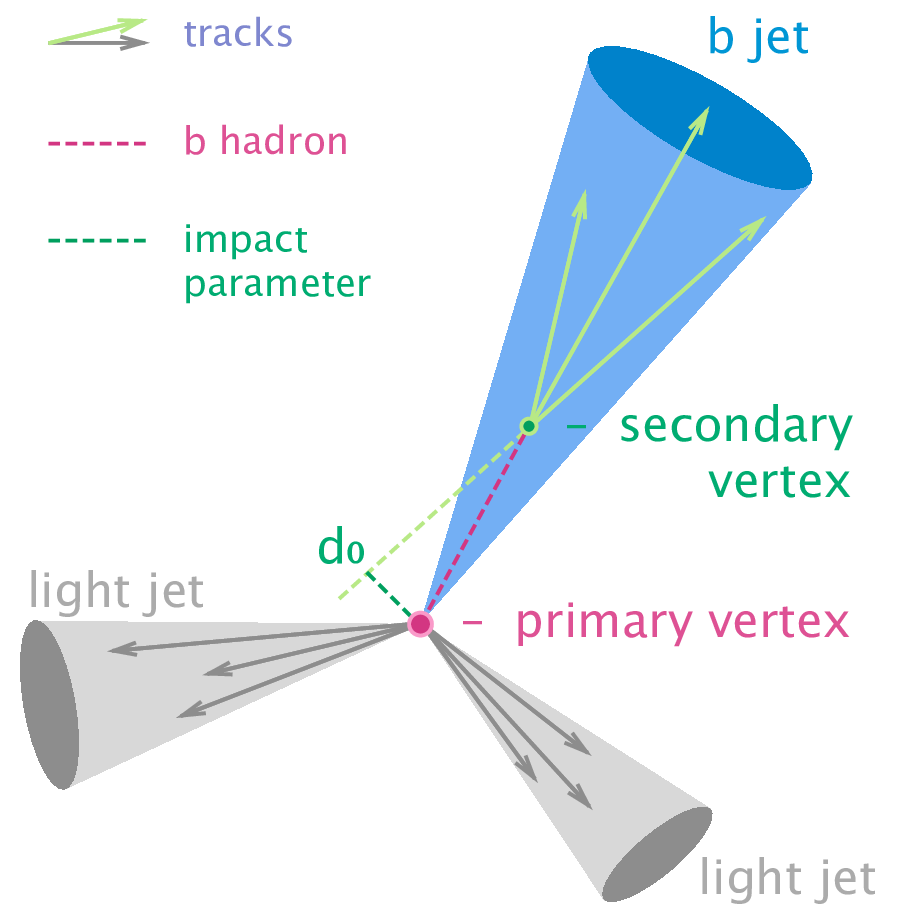
\includegraphics[width=.6\textwidth]{FTAG_plots/B-tagging_diagram.png}
	\caption{A diagram showning the b hadron decay initiated jets. }
	\label{fig:b-jet-decay}
	\end{centering}
\end{figure}


The strategy developed by the ATLAS Collaboration is based on a two-stage approach. 
Firstly, low-level algorithms reconstruct the characteristic features of 
the \bjets\ via two complementary approaches, a) that uses the 
individual properties of charged-particle tracks
associated with a hadronic jet, and b) that 
combines the tracks to explicitly reconstruct displaced vertices. 
These algorithms, first introduced during Run 1~\cite{PERF-2012-04}, 
have been improved and retuned for Run 2~\cite{FTAG-2018-01}. 
Secondly, in order to 
maximise the \btagging\ performance, the results of the low-level 
\btagging\ algorithms are combined into high-level algorithms 
via multivariate classifiers. 


The most performant algorithms presently in use in physics 
analyses at ATLAS are based on multivariate combinations 
of the available information (MV2) or additionally using a
deep feed-forward neural network (DL1)~\cite{tagging,ATL-PHYS-PUB-2017-013}, 
as shown in Figure~\ref{fig:b-tagging-performance}, where the performance
is characterised by the probability of 
tagging a \bjet\ (\bjet\ tagging efficiency, 
$\epsilon_b$) and the probability of mistakenly identifying 
a \cjet or a light-flavour jet as a \bjet\, 
labelled $\epsilon_c$($\epsilon_l$). 
In addition, the distribution of the output discriminant
of the MV2 and DL1 tagger for \bjet, \cjet, and light-flavour jets
in the \ttbar\ simulated events are shown in Figure~\ref{fig:b-tagging-score}.
Depending on the low-level algorithm, 
the DL1 tagger can be further separated into two taggers: DL1 and DL1r,
where the DL1 tagger uses traditional track-based impact parameter 
taggers IP2D and IP3D~\cite{ATL-PHYS-PUB-2016-012} 
and the DL1r tagger uses a Recurrent Neural Network Impact Parameter tagger 
(RNNIP)~\cite{ATL-PHYS-PUB-2017-013}. 
The calibration of DL1 and DL1r algorithms has been an original contribution 
of the author of this thesis and it is described in more detail in Chapter~\ref{sec:FTAG}.
The DL1r tagger is now the 
default \btagging\ algorithm used for flavour tagging in ATLAS.
% where performance of the algorithms is quantified 
% in terms of \bjet\ efficiency versus \cjet\ (light jet) rejections, defined as 
% 1/$\epsilon_c$ and 1/$\epsilon_l$. 


%Their high mass also leads to decay products with a larger transverse momentum relative to the jet axis with respect to the ones typically found in jets from light partons. Finally, heavy hadrons have a sizable branching ratio for semileptonic decays, hence the presence of soft leptons in the produced jets provides another tool for heavy jet identification. %The general strategy is to start with simple algorithms that exploits a particular property of b jets and progressively add more information to build moresophisticated algorithms. %The output of these algorithms consists in a discriminant value for each jet. Operating points are then defined as thresholds on the discriminant, designed to provide a determined efficiency for identifying b jets.
% Low-level $b$-taggingalgorithms fall into two broad categories. A first approach, implemented in the IP2D and IP3D algorithms~\cite{ATL-PHYS-PUB-2017-013}, or RNNIP~\cite{ATL-PHYS-PUB-2017-003} is inclusive and based on exploiting the large impact parameters of the tracks originating from the $b$-hadron decay. The second approach explicitly reconstructs displaced vertices. To maximise the $b$-tagging performance, low-level algorithm results are combined using multivariate classifiers. To this end, two high-level tagging algorithms have been developed. The first one,MV2\cite{ATL-PHYS-PUB-2017-013}, is based on a boosted decisiontree (BDT) discriminant, while the second one,DL1, is based on a deep feed-forward neural network(NN). These two algorithms are presented in fig .
\begin{figure}[bth]
	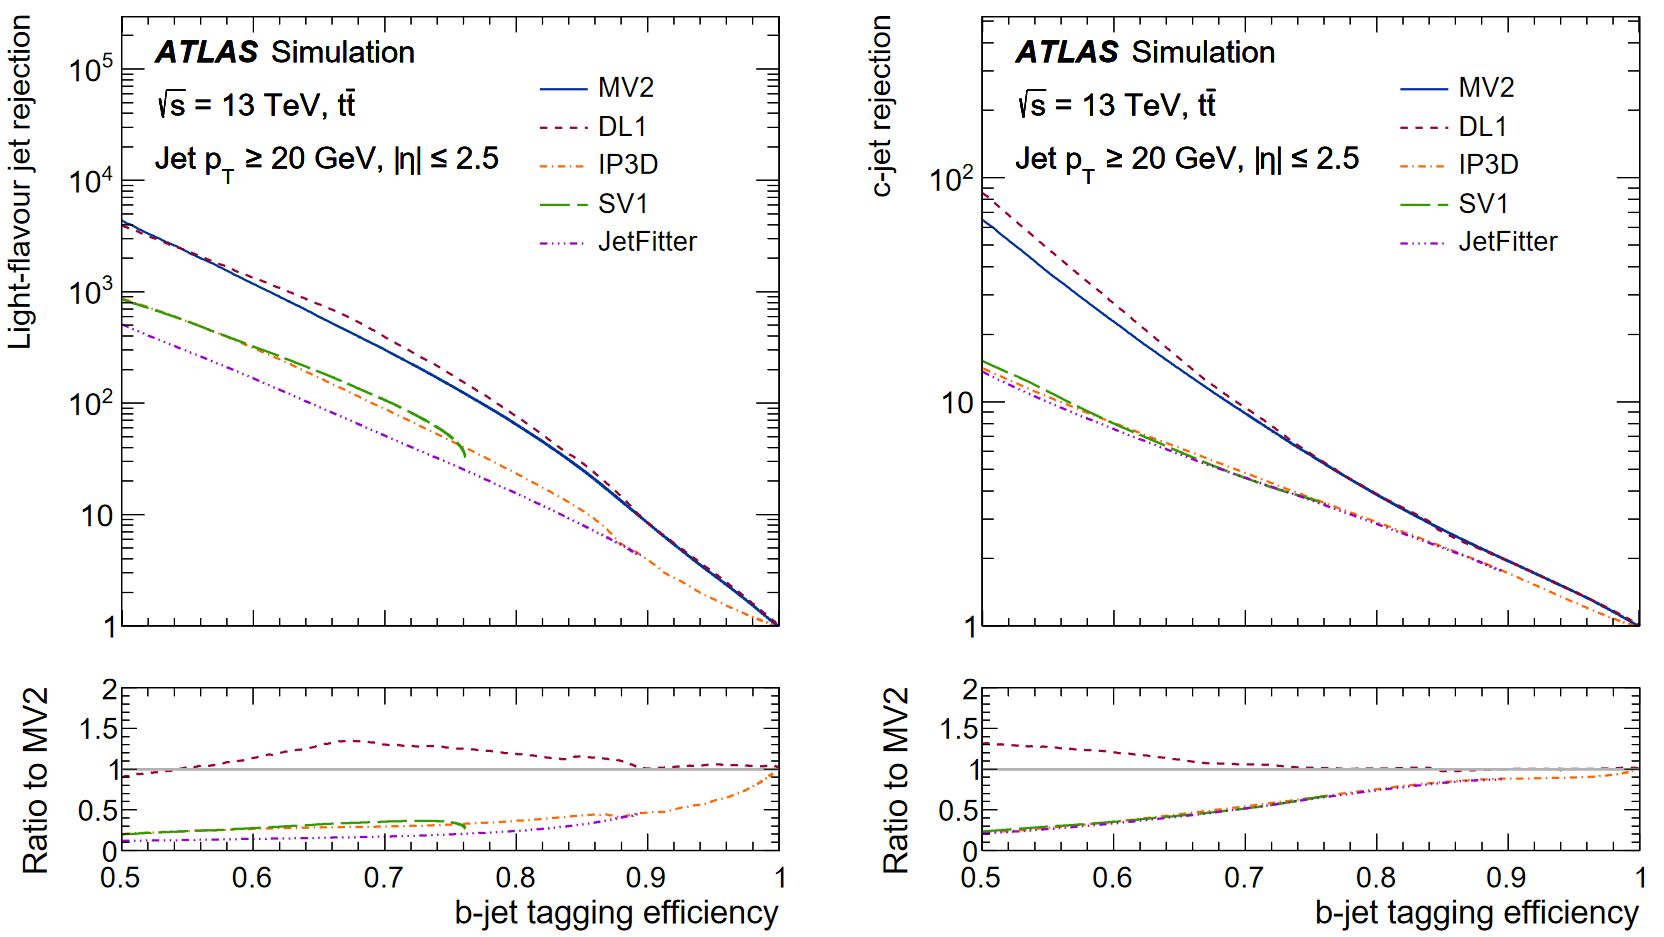
\includegraphics[width=.9\textwidth]{FTAG_plots/b-tagging-perfermance.png}
	\caption{The light-flavour jet (left) and \cjet\ (right) rejections versus 
	the \bjet\ tagging efficiency for the IP3D, SV1, JetFitter, MV2 and
	DL1 b-tagging algorithms evaluated on the \ttbar\ events
	~\cite{FTAG-2018-01}.}\label{fig:b-tagging-performance}
\end{figure}


\begin{figure}[bth]
	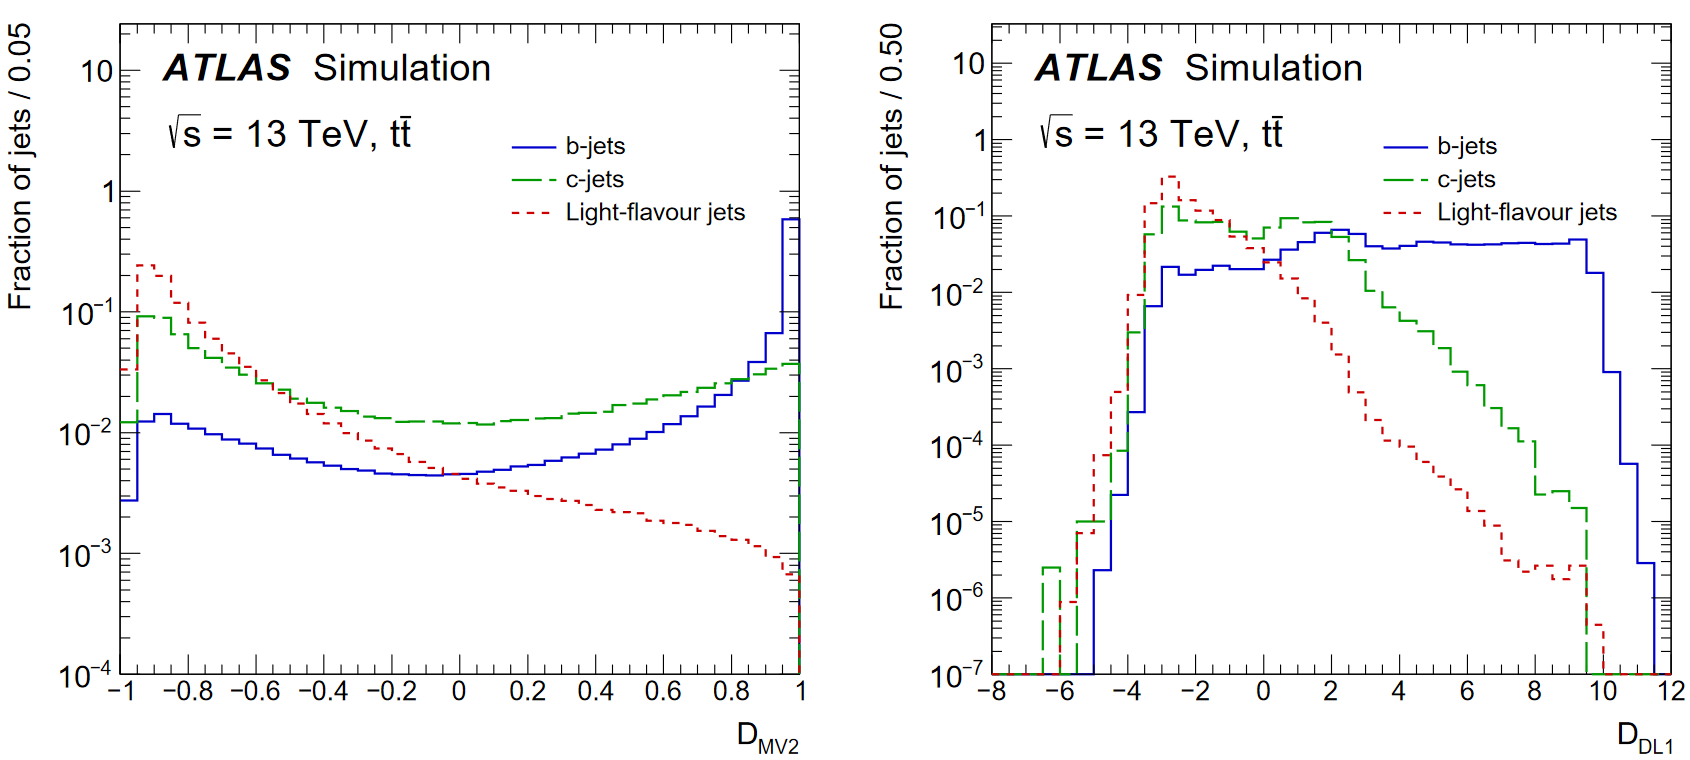
\includegraphics[width=.9\textwidth]{FTAG_plots/b-tagging-score.png}
	\caption{The fraction of light-flavour jets and \cjets\ versus 
	the \bjets\ in the MV2 (left) and
	DL1 (right) b-tagging algorithms output distribution 
	evaluated on the \ttbar\ events
	~\cite{FTAG-2018-01}.}\label{fig:b-tagging-score}
\end{figure}

\large

\section{Hadronically decaying $\tau$ lepton}
With a mass of 1.777 GeV and a proper decay length
of 87 $\mu$m~\cite{PDG}, tau leptons decay either leptonically
($\tau_{lep} \rightarrow \ell \nu \ell \nu \tau$, $\ell  = e, \mu$ ) 
or hadronically ($\tau_{had} \rightarrow$ hadrons $\nu_{\tau}$) 
and do so typically before reaching active
regions of the \hbox{ATLAS} detector. 
The leptonically decaying $\tau_{lep}$ is simply reconstructed
as either an electron or muon, with the netrinos contributing 
to the real component of the \met. 
On the other hand, the hadronically decaying $\tau_{tau}$ 
can be identified via their decay products. 
The hadronic tau lepton decays represent 65\% of all possible decay modes~\cite{PDG}. 
In these decay modes, the hadronic decay products are 
one or three charged pions in 72\% and 22\% of all cases, respectively. 
Charged kaons are present in the 
majority of the remaining hadronic decays. 
In 78\% of all hadronic decays, up to one associated neutral pion is
also produced. The neutral and charged hadrons stemming from 
the tau lepton decay make up the visible
decay products of the tau lepton, 
and are in the following referred to as $\tau_{had-vis}$.
\subsection{Reconstruction}
The $\tau_{had-vis}$ candidates are
seeded by jets formed using the anti-$k_t$ algorithm,
with a jet-size parameter $R$ of 0.4. 
For events with multiple interactions, the chosen primary may not be the
vertex where the tau lepton is originated. 
There the \textit{tau vertex association} algorithm is used with 
input as all tau candidates tracks within a region of $\Delta R$ < 0.2 
around the jet seed direction. 
The \pt\ of these tracks is summed and the 
primary vertex candidate to which the largest fraction
of the \pt\ sum is matched to is chosen as the tau vertex~\cite{ATLAS-CONF-2014-018}.

Tracks are associated with the $\tau_{had-vis}$ if they are
in the \textit{core} region $\Delta R$ < 0.2 
around the $\tau_{had-vis}$ direction and 
satisfy the following criteria: \pt\ > 1 GeV, 
at least two associated hits in the pixel layers of the inner detector, 
and at least seven hits in total in the pixel and the SCT layers. 
Furthermore, requirements are imposed on 
the distance of closest approach of the track to the track vertex
in the transverse plane, $|d_0|$ < 1.0 mm, and
longitudinally, $|z_0 sin\theta|$ < 1.5 mm. 
Tracks in the \textit{isolation} region 0.2 < $\Delta R$ < 0.4 
are used for the calculation of identification variables 
and are required to satisfy the same selection criteria.
% A set of boosted decision trees (BDTs) is used to classify all 
% tracks within $\Delta R$ = 0.4 of the $\tau_{had-vis}$ axis 
% into core and isolation tracks, depending on their \pt, 
% the number of hits in the tracking detectors 
% as well as their transverse and
% longitudinal impact parameters with respect to the tau vertex. 
The number of core tracks defines the number of \textit{prongs}.

\subsection{Identification}
The $\tau_{had-vis}$ reconstruction algorithm alone provides 
no discrimination against other particles that result in
jet-like signatures in the detector. 
Therefore, dedicated algorithms are used to identify hadronic tau lepton
decays. Here, a recurrent neural network (RNN) classifier 
is used as described in reference~\cite{ATL-PHYS-PUB-2019-033}.
Compared to the ID that was used in the analysis of the 36.1 fb$^{-1}$ data~\cite{HIGG-2016-16},
which was based on a boosted decision tree, 
the RNN tau-ID shows better performance 
and allows to move to a looser WP gaining increased efficiency 
(about 24\% and 11\% in case of two $\tau_{had}$ and 
one $\tau_{had}$ in the final state, respectively) 
without losing jet rejection, as shown in Figure~\ref{fig:RNNtau}. 
Due to the distinct signatures of 1- and 3-prong $\tau_{had}$ decays, 
the $\tau_{had}$--identification ($\tau_{had}$--ID) is split into dedicated
algorithms for 1- and 3-track $\tau_{had-vis}$.
Selected $\tau_{had-vis}$ candidates in the analysis are required to have 
\pt\ > 20 GeV, $|\eta|$ < 2.5, with candidates in the barrel-endcap 
transition region of the calorimeter (1.37 < $|\eta|$ < 1.52) vetoed 
due to poor detector instrumentation in this region, 
one or three tracks, unit charge, and to pass the ‘loose’ $\tau_{had}$--ID working point.
The loose WP corresponds to 85\% efficiency for 1-prong 
and 75\% efficiency for 3-prong (the efficiency is
flat in \pt\ by definition).
\begin{figure}[bth]
	\begin{centering}	
	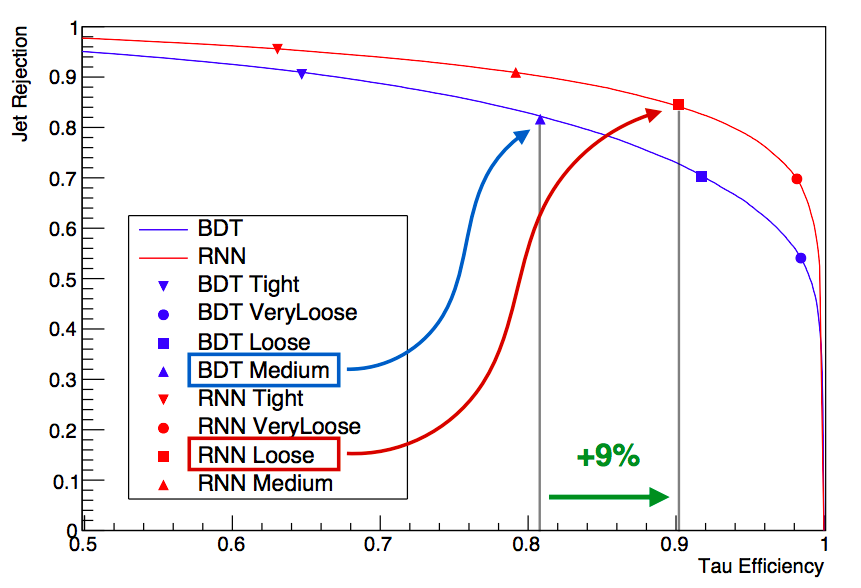
\includegraphics[width=.9\textwidth]{Reconstruction_plots/tauRNN.png}
	\caption{Jet rejection and tau efficiency of tau candidate, for BDT and
    RNN tau-ID.}
	\label{fig:RNNtau}
	\end{centering}
\end{figure}

Additional rejection of $\tau_{had-vis}$ candidates originating 
from electrons is provided by a BDT employing track
and shower shape information. 
The `loose' working point is used, corresponding to a selection efficiency
of about 95\% efficiency for true $\tau_{had-vis}$.
% Studies on the comparison between the BDT 
% (used in the previous round of the analysis) and RNN $\tau_{had}$--IDs
% and on the choice of the working point are reported in Appendix C.3. 

\section{Anti--$\tau_{had}$ definition}
In order to provide fake--$\tau_{had}$--enriched regions used for background estimation, 
an ``anti--$\tau_{had}$'' selection is defined. 
Those $\tau_{had-vis}$ objects that fail the RNN loose $\tau_{had}$--ID 
and have the RNN score greater than 0.01 are labelled as anti--$\tau_{had}$ candidates. 
For channels where $\tau_{had}$--ID is applied at trigger level, anti--$\tau_{had}$
candidates are also required to be matched to the trigger $\tau_{had}$ in 
the same way as is required for signal taus.
This definition selects objects that are 
predominantly jets faking hadronic $\tau$ decays. 
The minimum RNN score requirement ensures that 
the jets still have some $\tau_{had}$-like properties 
and ensures that the composition of quark- and gluon-initiated jets 
is closer to that of the signal region.
More details of the choice of the minimum $\tau_{had}$--ID RNN-score
threshold are reported in TODO: link to the fake factor section
% RNN score < 0.01 is chosen as it is the cut used and recommended by the Fake-Tau-Task-Force and was
% also tested here to give an improvement in the statistical precision of the multi-jet fake-factors and of the
% multi-jet template compared to the "VeryLoose" working point (RNN score < 0.05, with 95\% efficiency
% for true-$\tau_{had}$).
% Internal note C.4.1:
% The RNN > 0.01 is used by the Fake-Tau-Task-Force and has been studied here to extend the anti-tauhad
% 2526 control regions and check the impact of the reduced statistical uncertainties on the FFs and of the reduced
% 2527 statistical uncertainties on the multi-jet template.
% 2528 Lowering the cut from RNN > 0.05 of the VeryLoose to RNN > 0.01 gives an improvement in the
% 2529 statistical precision of the FFs (about 10-15% reduction in relative uncertainty) which translates in smaller
% 2530 systematic uncertainties from this source on the multi-jet template and more importantly it reduces the
% 2531 statistical uncertainty on the multi-jet tempalte itsfelf by reduced by approximately 30% given the increased
% 2532 statistics in the Anti-ID OS region where the FFs are applied to obtain the template for the SR, as shown in
% 2533 Figure 166.
\subsection{Anti--$\tau_{had}$ selection}
Anti--$\tau_{had}$ objects are selected only in events 
in which there are fewer $\tau_{had}$ that pass the offline $\tau_{had}$--ID than
required for a given channel (one for the $\tau_{lep}\tau_{had}$ 
and two for the $\tau_{had}$$\tau_{had}$ selection). 
In that case, additional anti--$\tau_{had}$ candidates are selected 
so that the total number of selected $\tau_{had}$ (loose, which always has priority,
and anti--$\tau_{had}$) corresponds to the required multiplicity in each channel.
For channels where $\tau_{had}$--ID is applied at trigger level 
(more details in Section~\ref{sec:event selection}), 
only the anti--$\tau_{had}$ objects that are matched to the
trigger $\tau_{had}$ are considered, and thus there are 
no multiple selection possibilities. 
However, for channels where a $\tau_{had}$ trigger is not used, 
an anti--$\tau_{had}$ candidate is chosen randomly when there are more reconstructed
$\tau_{had}$ satisfying the anti--$\tau_{had}$ definition. 
Any anti--$\tau_{had}$ objects that are not selected in this process are also not
considered when performing the overlap removal of detector objects, 
which is discussed in Section~\ref{sec:overlap}.

\section{Missing transverse energy}
As defined in Equation~\ref{eq:MET}, the $\vec{E_T}^{miss}$ is defined 
as the negative vector sum of transverse momentum collected from the 
detector, from which one or more ``invisible'' particle(s) can be inferred. 
The reconstruction of $\vec{E_T}^{miss}$ is comprised of two contributions~\cite{MET2018}. 
The first one is from \textit{hard-event} signals combining 
information of fully reconstructed and calibrated 
physics objects, i.e. electrons, muons, photons, jets,
hadronically decaying $\tau$-leptons and jets. 
The second one is from the \textit{soft-event}, consisting of 
reconstructed charged-particle tracks associated with the hard-scatter
vertex but with no physics objects.

\section{Overlap removal}
After the event is reconstructed, an overlap-removal procedure is applied 
to resolve ambiguities when a physical object is reconstructed as multiple 
particles in the \hbox{ATLAS} detector. The angular distance $\Delta R$ is used 
to measure the overlap of two reconstructed objects.
Overlaps between most of the detector objects used in the analysis are resolved 
by using the standard overlap removal tools AssociationUtils~\cite{ORTool}, 
with analysis specific procedure for 
the reconstructed $\tau_{had-vis}$, anti-$\tau_{had-vis}$ objects and jets.
The step-by-step procedure that is used to resolve ambiguities in the 
reconstructed objects is summarised in  the following:
 \begin{itemize}
     \item  $e_1$--$e_2$: For two electrons $e_1$ and $e_2$ in an event,  
     reject $e_1$ if both electrons share the track and $p_{T1}$ < $p_{T2}$
    \item  $\tau_{had-vis}$--$e$: Reject $\tau_{had-vis}$ if $\Delta R$ < 0.2 
    % and   $e$ passes \hbox{DFCommonElectronsLHLoose}
    \item  $\tau_{had-vis}$--$\mu$: Reject $\tau_{had-vis}$ if $\Delta R$ < 0.2:
     \\ Case 1 ($\tau_{had-vis}$ $p_T$ > 50GeV): $p_T$, $\mu$ > 2GeV and combined muon
     \\ Case 2 ($\tau_{had-vis}$ $p_T$ $\leq$ 50GeV): $p_T$, $\mu$ > 2GeV
    \item  $\mu$--$e$: Reject $\mu$ if calo-muon and shared ID track
    \item  $e$--$\mu$: Reject $e$ if shared ID track
    \item  jet--$e$: Reject jet if $\Delta R$ < 0.2
    \item  $e$--jet: Reject $e$ if $\Delta R$ < 0.4
    \item  jet--$\mu$: Reject jet if $N_{track}$ < 3 ($p_{T}^{track}$ > 500MeV), and $\Delta R$ < 0.2
    \item  $\mu$--jet: Reject $\mu$ if $\Delta R$ < 0.4
 \end{itemize}
 Additionally, an analysis-specific overlap-removal procedure for $\tau_{had-vis}$, 
 anti-$\tau_{had-vis}$ and jets is implemented:
\begin{itemize}
    \item jet--$\tau_{had-vis}$: Reject jet if $\Delta R$ < 0.2
    \item anti--$\tau_{had-vis}$--jet: Reject anti--$\tau_{had}$ if jet is $b$-tagged and $\Delta R$ < 0.2
    \item jet--anti--$\tau_{had-vis}$: Reject jet if $\Delta R$ < 0.2
\end{itemize}
 This establishes the following priority: $\tau_{had-vis}$ > $b$-tagged jet > anti-$\tau_{had-vis}$ > un-tagged jet.
%  Another priority, $b$-tagged jet > $\tau_{had-vis}$ > anti-$\tau_{had-vis}$ > un-tagged jet, was investigated as an alternative
%  but found to reduce signal acceptance in the 2-tag region significantly due to limited $\tau_{had}$ rejection of the
%  DL1r $b$-tagging algorithm at the 77\% working point. With the alternative priority the signal acceptance is
%  reduced by about 8\% (13\%) in $\tau_{lep}$$\tau_{had}$ ($\tau_{had}$$\tau_{had}$).
\label{sec:overlap}

 
\chapter{Charm jet mis-tagging calibration}
\label{sec:FTAG}
\section{Calibration methods for \bjet\ and light jet}
\large
MC simulations are not able to model exactly the 
performance of the $b$-tagging algorithms in data. For this reason 
calibration is required, i.e.\ correcting MC to recover the data 
in terms of $b$-tagging efficiency, charm jet mis-tagging and 
light jet mis-tagging rates~\cite{FTAG-2018-01}. The calibration is performed 
for all supported jet collections(TODO: refer back to the object definition chapter)
and working points, which are cuts in the \btagging\ 
algorithm output identifying the different tagging efficiencies 
and corresponding light jet and \cjet rejection rate.
In general, the efficiency is calculated with data and simulations, 
and scale factors are then calculated to match the efficiency extracted 
from simulations to the data.
% The imperfect 
% description of the detector response and physics modelling effects 
% in Monte Carlo (MC) simulations necessitates the measurement of the 
% performance of the \btagging\ algorithms with collision data 
%~\cite{PERF-2012-04,ATLAS-CONF-2018-045}. 
% The measurement of the \bjet\ tagging efficiency 
% of the high-level \btagging\ algorithms used in proton–proton (pp) 
% collision data recorded during Run 2 of the LHC at $\sqrt{s}$ = 13 TeV 
% is presented. 
% The corresponding measurements for \cjets\ and light-flavour 
% jets, used in the measurement of the \bjet\ tagging efficiency to correct 
% the simulation such that the overall tagging efficiency of \cjets\ and 
% light-flavour jets match that of the data, are described elsewhere 
%~\cite{ATLAS-CONF-2018-006},~\cite{cjet}. 
The production of $t\bar{t}$ 
pairs at the LHC provides an abundant source of \bjets by virtue 
of the high cross-section and the $t \rightarrow Wb$ branching ratio 
being close to 100\%. A very pure sample of $t\bar{t}$ events can be 
selected by requiring that both $W$ bosons decay leptonically, 
referred to as di-leptonic $t\bar{t}$ decays in the following.
For the \bjet\ calibration, the performance of the $b$ tagging 
algorithms is evaluated in the simulation and the efficiency 
with which these algorithms identify jets containing $b$-hadrons 
is measured in collision data. The measurement uses a likelihood-based 
method in the di-leptonic $t\bar{t}$ sample, where
events with exactly 2 jets and 2 opposite-sign leptons are selected.  
The data \bjet\ efficiency is 
then extracted from a combined likelihood fit, and subsequently 
compared with that predicted by the simulation. Scale factors are 
then calculated to emulate the performance of the algorithms to the data~\cite{FTAG-2018-01}.

For the light jet mis-tagging calibration, two methods are 
used to measure the mis-tagging rate from the data~\cite{ATLAS-CONF-2018-006}. 
The first is the negative tag method, which uses a high statistics data sample enriched 
in light jets with the application of a modified algorithm which 
reverses some of the criteria used in the nominal identification 
algorithm.
The second is the adjusted Monte Carlo (adjusted-MC) method, which 
adjusts the characteristic track observables in the simulation 
to im the data, and then compares the adjusted simulation to the 
``standard'' simulation. The scale factors are then calculated using 
the these two methods. The scale factors of the two different methods 
are in good agreement within the systematic uncertainties. 
%The aim of this calibration is to calibrate \bjets that have been mis-tagged as light jets of \btagging\ algorithm. As the $b$-tagging algorithm is very efficient in rejecting light jets, the light jet fraction is enriched via ``flipped'' taggers, which negates the sign of track IP parameters before $b$-tagging\cite{ATLAS-CONF-2018-006}. The calibrations of the standard and the 'flipped' tagger are assumed to be equal. The calibration is extracted using the leading $p_T$ jet of Z+jets events using a 2D fit. TODO: cite the light jet tagging Int note
%light jet fractions in the $b$-like region are too low,  The Z + jets events are then selected, the secondary vertex mass is fitted to obtain flavour fractions and perform a likelihood fit to extract light jet mistag rate.
\section{Calibration method for \cjet}
\label{sec:Calibration method for charm jet}
It is worth mentioning that the author's qualification task to become an ATLAS author is to 
calibrate the rate of a charm jet being mis-identified as a \bjet\, which is a part 
of the calibration of the $b$-tagging algorithm.
During the task the calibration range has been extended down to 20~GeV (previously 25~GeV) in
jet \pt\ and a new selection category has been developed 
to increase the data statistics of the scale factors in the 
high-$p_T$ ($p_T^{jet}$ > 70~GeV) region.
The calibration is performed on the PFlow jets (as defined in Section~\label{sec:jet})
and \textit{VR-Track jets} reconstructed using the variable radius jet algorithm~\cite{VRTrackJet}.

As determined by the CKM matrix~\cite{CKM1,CKM2}, the $W$ boson decays dominantly to 
a pair of light quarks ($u$ quark and $d$ quark) or to
a $s$ quark and a \cquark. The $W$ boson decays very rarely to pairs containing a \bquark. 
More specifically, the branching ratio of a $W$ boson decays to a $u$ quark and $d$ quark pair or 
a $s$ quark and $c$ quark pair is 33.1\%, and to pairs containing a $b$ quark is only 0.057\%~\cite{PDG}. 
Therefore, $b$-tagged jets from the $W$ decay are most likely 
to be mis-tagged \cjets or light jets. 

Furthermore, given the ratio between the DL1 light jet rejection and the corresponding charm jet rejection 
ranges from 10 to 40 (Figure~\ref{fig:b-tagging-performance}), the 
\cjet\ is much more likely to be mis-tagged than the light jet. 
This allows for a source of mis-tagged \cjets to be obtained in the \ttbar\ events, 
requiring that one $W$ boson decays leptonically and the other decay hadronically 
(referred to as semi-leptonic $t\bar{t}$ decay in the following),
where the $b$-tagged jets from the $W$ decay are candidates of mis-tagged \cjets.
Requiring a $W$ boson decaying leptonically 
reduces the number of combinations of jets of different flavour, 
and allows triggering with the lepton.

The events kinematics are shown by the diagram in 
Figure~\ref{fig:feynman}, where the \ttbar\ pair decays to a 
$b$ and a $\bar{b}$ quark, circled in red. One of the $W$ bosons, 
circled in blue, decays hadronically to quarks, 
and the other $W$ boson decays leptonically to either 
an electron or a muon and the corresponding neutrinos, 
circled in green and purple, respectively. 
The lepton in the final state is used for triggering.
The following notation will be used: the jets that are
the decay products of the $W$ boson are referred to as
$W$ jets and the remaining two jets are referred to as top-jets.

\begin{figure}[H]
\centering
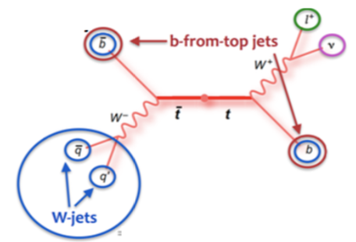
\includegraphics[width=.45\textwidth]{FTAG_plots/feynman.png}
\caption{Feynman diagram of the semi-leptonic $t\bar{t}$ events.}
\label{fig:feynman}
\end{figure}

%As Shown in Fig \ref{fig:feynman}, the calibration uses the semi-leptonic $t\bar{t}$ events, which one $W$ boson from top decays leptonically to a charged lepton and neutrino and one $W$ decays hadronically and dominantly to a charm and a strange quark, among other pairs.

A kinematic likelihood technique, referred to as 
KLFitter~\cite{ERDMANN201418}, is used to assign jets to the proper $t\bar{t}$ decay product 
(more details in Section \ref{KLFitter}). 
The following notation will be used: the jets that are
assigned as the decay products of the $W$ boson are referred to as
$W$ jets and the remaining two jets are referred to as top jets.


The charm jet efficiency is defined as the ratio of events with either of the 
\wjet\ is tagged. The efficiency is evaluated in four \pt\ intervals, with 
boundaries of 20, 40, 65, 140 and 250~GeV for the PFlow jets and 15, 20, 40, 140~GeV
for the VR-Track jets; and for four tagging intervals with the boundaries of 85\%, 77\%,
70\% and 60\%. 

The choice of the bin boundaries ensures enough statistics for each bin and 
hence relatively flat statistical uncertainty, 
given the underlying charm-jet \pt\ spectrum as shown in Figure~\ref{fig:kinematic_distributions_combined}.
The boundaries for the VR-Track jets are lower than for PFlow jets, 
since the track jets miss the neutral particles the
reconstructed energy is significantly below the true jet energy.

The main method described in the chapter is for the ``fixed-cut'' calibration
where the efficiency is defined as the fraction of \bjets passing the tagger.
Jets are said to be tagged (untagged) at particular working point
if they have DL1r scores greater (less) than the DL1r score of that working point.
The events with both \wjet\ are discarded to simplfiy the fit described in the following.

To extract the scale factors of the charm jet mis-tagging, a fit is performed by minimising 
the $\chi^2$ defined as:
\begin{eqnarray*}
\chi^2 = \sum_{t=1}^4 \sum_{i=1}^4  \sum_{j=1}^4 (N^{t}_{\mathrm{data}}(i,j)- p(i,j) [c^{t}(i)N^{t}_{C}(i,j)+N^{t}_{J}(i,j)
\end{eqnarray*}
\begin{eqnarray*}
	+ \sum_k  c^{4}(k) N^{t}_{X}(i,j,k)])^2/N^{t}_{\mathrm{data}}(i,j)
\end{eqnarray*}
\begin{eqnarray}
 +  \sum_{i=1}^4 \sum_{j=i}^4 [N^{\mathrm{untag}}_{\mathrm{data}}(i,j)-p(i,j)N^{\mathrm{untag}}_{\mathrm{MC}}(i,j)]^2/N^{\mathrm{untag}}_{\mathrm{data}}(i,j).
\label{eqn:chi2}
\end{eqnarray}
The $c^{t}(i)$ is the main floating parameter in the fit, which is the charm jet 
mis-tagging scale factor at working point $t$ of \pt\ bin labelled $i$. 
The other main floating parameter is $p(i,j)$ that is the normalisation factor scaling the MC to
data. 
The $N^{t}_{\mathrm{data}}(i,j)$ is the number of data events with a tagged \wjet\ in the \pt\ bin labelled i
and the other (untagged) \wjet\ in the \pt\ bin labelled j. Similarly the $N^{t}_{C}(i,j)$ is the number of MC events 
with a tagged \wjet\, while the tagged \wjet\ is indeed a \cjet\, which can be seen as ``signal''. 
In contrast the $N^{t}_{J}(i,j)$ is the number of events with neither the tagged \wjet\ nor the top jets 
are \cjets\; and the $N^{t}_{X}(i,j,k)$ is the number of events with one of the top jets is a \cjet\. 
These two types of events can be seen as ``background''. The later case is slightly more complicated, as the 
\cjet\ lies in a different \pt\ bin to the tagged jet, denoted as $k$, and it only depends on the 
$c^4(k)$ (which is the scale factor of the 4th working point i.e. 60\% ) as the top jets
are tagged at 60\% working point. 
The calibration is then given as the scale factors of the four working points 
in bins of \pt\ defined in the above text. 

% The charm-jet efficiency of the MC can be extracted from the truth information which indicates the 
% true nature of the $W$ jets. The \cjet\ efficiency of the MC is defined as the probability a true \cjet\ 
% is tagged by the \btagging\ algorithm in bins of jet \pt. 
% The charm-jet efficiency of the data is extracted by applying a combinatorial likelihood fit to $W$ jets, 
% where the main floating parameter are the \cjet\ efficiency
% in a given \pt\ bin and the ratio of data over total MC. 
% The calibration is given as scale factors in bins of \pt\ for 4 fixed-cut working points (WP) 
% that scale the simulation shape to reproduce that of the data, where the
% scale factors are calculated as the ratio of the data charm-jet efficiency over 
% the MC charm-jet efficiency. The calibration is performed for 4 \pt\ bins  
% (20, 40, 65, 140, 250) for the PFLow jets and (10, 20, 40, 65, 140) for the VR-Track jets
% in units of GeV. 

\section{Data and Monte Carlo samples}
%%%%%%%%%%%%%%%%%%%%%%%%%%%%%%%%%%%%%%%%%%%%%%%
\label{sec:samples}
TODO: remove the overlap between this section and the Data MC chapter in the thesis
Dedicated MC are used to model SM processes. 
%%%%%%%%%%%%%%%%%%%%%%%%%%%%%%%%%%%%%%%%%%%%%%%
The data analysed in this study correspond to 139~fb$^{-1}$~\cite{DAPR-2010-01,DAPR-2011-01,DAPR-2013-01,LUCID2}, 
of \(pp\) collision data collected by the ATLAS detector between 2015 and 2018
with a centre-of-mass energy of 13~\TeV. 
The data sample was collected using a set of single-muon~\cite{Aad:2020uyd} 
and single-electron triggers~\cite{TRIG-2018-05}. The single-muon triggers 
had \pt\ thresholds in the range 20--26~\GeV\ for 
isolated muons and 50~\GeV\ for muons without any isolation requirement. 
The single-electron triggers employed a range of \pt\ thresholds 
varying between 24--300~\GeV\ 
and a combination of quality and isolation requirements depending on the 
data-taking period and the \pt\ threshold.
%The uncertainty in the combined 2015--2018
%integrated luminosity is 1.7\%~\cite{ATLAS-CONF-2019-021}, obtained
%using the LUCID-2 detector~\cite{LUCID2} for the primary luminosity
%measurements. 
All detector subsystems were required to be operational
during data taking and to fulfil data quality requirements.  

% The $t\bar{t}$ samples and the single top-quark in the Wt 
% and s-channel samples are generated with the {\tt Powheg-Box} v2~\cite{powheg} 
% generator. Electroweak t-channel single top-quark events are generated 
% using the {\tt Powheg-Box} v1~generator. The parton shower, fragmentation, 
% and the underlying event are simulated using {\tt Pythia} 6.428\cite{pythia} 
% with the CTEQ6L1 PDF sets and the corresponding Perugia 2012 tune (P2012)~\cite{perugia}. 
% The top-quark mass is set to 172.5~GeV. The {\tt EvtGen} v1.2.0 program~\cite{evtgen} 
% is used to model the properties of the bottom and charm hadron decays. 
% The $t\bar{t}$ production cross-section is calculated at NNLO+NNLL 
% (next-to-next-to-leading-logarithm)~\cite{NNLO}. For single-top processes, 
% the generator NLO cross-sections are used. Events containing $W$ or $Z$ 
% bosons with associated jets are simulated using {\tt Sherpa} 2.2.1\cite{sherpa}. 
% All $W$/$Z$+jets events are normalised to the predicted cross-sections using 
% NNLO calculations. All samples are passed through the full GEANT4\cite{GEANT4} 
% simulation of the ATLAS detector and are reconstructed with the same software as used for data.



All samples were 
produced using the ATLAS simulation infrastructure~\cite{SOFT-2010-01}
and $\GEANT4$~\cite{Agostinelli:2002hh}. A subset of samples use a faster 
simulation based on a parameterisation of the calorimeter response and 
$\GEANT4$ for the other detector systems~\cite{SOFT-2010-01}. %\cite{ATL-PHYS-PUB-2010-013}.
The simulated events are reconstructed with the same algorithms as
used for data, and contain a realistic modelling of pile-up
interactions. The pile-up profiles in the simulation match those of each dataset
between 2015 and 2018, and are obtained by overlaying minimum-bias events,
simulated using the soft QCD processes of
{\PYTHIA}~8~\cite{Sjostrand:2014zea} using the NNPDF2.3LO set of
PDFs~\cite{Ball:2012cx} and a set of tuned
parameters called the A3 tune~\cite{ATL-PHYS-PUB-2016-017}.

The events that are used in this study originate mostly due to 
\ttbar\ production. This process is modelled using the
\powhegbox~v2~\cite{Frixione:2007nw,Nason:2004rx,Frixione:2007vw,Alioli:2010xd}
generator at NLO with the \nnpdfnlo % ~\cite{Ball:2014uwa}
parton distribution function (PDF) set
and the \hdamp\ parameter\footnote{The
  \hdamp\ parameter is a resummation damping factor and one of the
  parameters that controls the matching of \powheg matrix elements to
  the parton shower and thus effectively regulates the
  high-\pt\ radiation against which the \ttbar\ system recoils.} set
to 1.5~\mtop~\cite{ATL-PHYS-PUB-2016-020}.  The events were interfaced
to {\PYTHIA}~8.230 to model the parton shower,
hadronisation, and underlying event, with parameters set according
to the A14 tune and using the \nnpdftwo set of PDFs.
The decays of bottom and charm hadrons were performed by \evtgen~v1.6.0~\cite{EvtGen}.
 The simulated \ttbar\
events are split according to the origin of $W$ jets. The notation
``\ttbar, ll'' denotes that both $W$ jets are light flavour jets.
Similarly, ``\ttbar, cl'' (``\ttbar, bl'') 
indicates that one of the $W$ jets is a \cjet\ (\bjet)
whereas the other is a light flavour jet. $W$ jets with origin
other than what is discussed above fall into the 
category denoted by ``\ttbar, other''. This category includes
events in which at least one of the $W$ jets comes from a
hadronically decaying $\tau$-lepton. 

%%% single top
In addition to \ttbar\ production, there are some minor backgrounds
that contribute to the final event sample that is used for the calibration.
These backgrounds consist mostly of single-top and diboson production, 
the production of \ttbar\ in association with a vector boson
and the production of a vector boson in association with jets.
The details
of the modeling of these samples are given in the following.

Single-top $s$-channel production is modelled using the \powhegbox~v2 %~\cite{Alioli:2009je,Nason:2004rx,Frixione:2007vw,Alioli:2010xd}
generator at NLO in QCD in the five-flavour scheme with the \nnpdfnlo~\cite{Ball:2014uwa} parton distribution function~(PDF) set.
%The events are interfaced with \pythia.230 % ~\cite{Sjostrand:2014zea} 
%using the A14 tune % ~\cite{ATL-PHYS-PUB-2014-021}
%and the \nnpdftwo PDF set.
%
The associated production of top quarks with $W$ bosons ($tW$) is
modelled using the
\powhegbox~v2~\cite{Re:2010bp,Nason:2004rx,Frixione:2007vw,Alioli:2010xd}
generator at NLO in QCD using the five-flavour scheme and the
\nnpdfnlo set of PDFs~\cite{Ball:2014uwa}.
The diagram removal scheme~\cite{Frixione:2008yi} is used to
remove interference and overlap with \ttbar\ production. 
The events for both single-top $s$-channel and $tW$ production 
are interfaced to \pythia.230%~\cite{Sjostrand:2014zea} 
using the A14 tune%~\cite{ATL-PHYS-PUB-2014-021} 
and the \nnpdftwo set of PDFs. %~\cite{Ball:2012cx}.

The production of $Z+$jets and $W$+jets is simulated with the
\sherpa~v2.2.1~\cite{Bothmann:2019yzt}
generator using next-to-leading order (NLO) matrix elements (ME) for up to two partons, and leading order (LO) matrix elements
for up to four partons calculated with the Comix~\cite{Gleisberg:2008fv}
and \openloops~\cite{Buccioni:2019sur,Cascioli:2011va,Denner:2016kdg} libraries. They
are matched with the \sherpa parton shower~\cite{Schumann:2007mg} using the MEPS@NLO
prescription~\cite{Hoeche:2011fd,Hoeche:2012yf,Catani:2001cc,Hoeche:2009rj}
using the set of tuned parameters developed by the \sherpa authors.
The \nnpdfnnlo set of PDFs~\cite{Ball:2014uwa} is used and the samples
are normalised to a next-to-next-to-leading order (NNLO)
prediction~\cite{Anastasiou:2003ds}.

Samples of diboson final states ($VV$) are simulated with the
\sherpa~v2.2.1 or v2.2.2~\cite{Bothmann:2019yzt} generator depending on the process,
%~\footnote{This is an admixture of 2.2.1 and above versions, so the version should be kept generic to avoid confusions. As an alternative, the sentence can be modified indicating that samples are simulated with the \sherpa~v2.2.1 or v2.2.2 depending on the process.} 
including off-shell effects and Higgs-boson contributions, where appropriate.
Fully leptonic final states and semileptonic final states, where one boson
decays leptonically and the other hadronically, are generated using
matrix elements at NLO accuracy in QCD for up to one additional parton
and at LO accuracy for up to three additional parton
emissions. Samples for the loop-induced processes $gg \to VV$ are
generated using LO-accurate matrix elements for up to one
additional parton emission for both cases of fully leptonic and
semileptonic final states. The matrix element calculations are matched
and merged with the \sherpa parton shower based on Catani-Seymour
dipole factorisation~\cite{Gleisberg:2008fv,Schumann:2007mg} using the MEPS@NLO
prescription~\cite{Hoeche:2011fd,Hoeche:2012yf,Catani:2001cc,Hoeche:2009rj}.
The virtual QCD correction are provided by the
\openloops library~\cite{Buccioni:2019sur,Cascioli:2011va,Denner:2016kdg}. The
\nnpdfnnlo set of PDFs is used, %~\cite{Ball:2014uwa}, 
along with the dedicated set of tuned parton-shower parameters developed by the
\sherpa authors.

The production of \ttbar\ in assosiation with a vector boson 
is modelled using the
\mgamc~v2.3.3~\cite{Alwall:2014hca} generator at NLO with the
\nnpdfnlo~\cite{Ball:2014uwa} parton distribution function~(PDF).
The events are interfaced to \pythia.210~\cite{Sjostrand:2014zea}~
using the A14 tune~\cite{ATL-PHYS-PUB-2014-021} and the
\nnpdftwo~\cite{Ball:2014uwa} PDF set. The decays of bottom and charm
hadrons are simulated using the \evtgen\ v1.2.0 program~\cite{Lange:2001uf}.



\section{Kinematic Likelihood Fitter}
\label{KLFitter}
% Top quarks decay to a $W$ boson and a bottom quark in nearly 100\% of all 
% cases. Consequently, the final state of a top-quark pair is characterised by 
% the decay products of the two $W$ bosons. 
% %If one of the $W$ bosons decays into a charged lepton and a neutrino while the other one decays into a pair of quarks, the decay mode is referred to as the single-lepton, or semi-leptonic decay mode. 
% The fraction of top-quark pairs decaying either in the 
% single-electron or single-muon decay mode 
% is about 30\%. The corresponding event signature is defined 
% by exactly one electron or muon, four jets out of which 
% two contain a $b$-hadron, and a large amount of missing transverse momentum 
% due to the un-detected neutrino. The Kinematic Likelihood Fitter\cite{ERDMANN201418}, 
% is a reconstruction technique developed to reconstruct $t\bar{t}$ decays, 
% which exploits the above decay topology of the top quark in the 
% semi-leptonic channel in order to properly associate jets to the 
% quarks in the final state of the decay process. In the semi-leptonic 
% decay of the $t\bar{t}$ system, the resulting tree level situation 
% contains two $b$ quarks from the top quark decays, and two light or 
% charm quarks from the $W$ boson decay (Figure~\ref{fig:feynman}). 
% A likelihood is used to properly assign these four jets to the true 
% decay quarks. The leading order scenario is assumed, giving rise to four jets 
% in the final $t\bar{t}$ decay topology, two of which are \bjets. Three 
% of the jets in the decay are associated to the hadronic top decay, 
% whereas a final fourth jet along with the charged lepton and 
% neutrino build the leptonic top\cite{cjet}.
The four-vectors of the four highest \pt\ jets, the lepton and the
event \MET\ are used as inputs to a likelihood-based \ttbar\ event
reconstruction algorithm, which is described in more detail in
Ref.~\cite{ERDMANN201418}. This algorithm uses a likelihood function
to assign the four jets to the \ttbar\ decay topology. In particular,
the algorithm assigns one jet to be the \bjet\ from the leptonically
decaying top quark ($t\to Wb \to \ell \nu b$), another to the \bjet\
from the hadronically decaying top quark ($t\to Wb \to qq^\prime b$,
where $qq^\prime$ are the quarks in which the $W$ boson decays) and
the remaining two jets to the jets that come from the hadronic $W$
boson decay. The jet assignment does not use any \btagging\ information
to avoid bias.



\section{Maximising likelihood}
\label{maximise likelihood}
Taking only four jets in the event limits the total number of possible 
jet orderings (permutations) in the event. In the semi-leptonic channel, 
four jets can be permuted a total number of times equal to 4! = 24. 
However, the two $W$ jets are kinematically indistinguishable. 
This reduces the possible number of permutations to 12. 
%Furthermore, no $b$-tagging information is used 
%in the kinematic likelihood to limit the possible number of permutations
%as this would bias the result.
For every combination of jet ordering, 
the likelihood is maximised over 
its free parameters, the energy of the four jets, the lepton energy and 
the three components of the momentum of the neutrino, and provides a 
value based on how closely the kinematic information from the reconstructed 
objects for a specific jet ordering resembles the expected kinematic behaviour 
of the decay of a Standard Model semi-leptonic $t\bar{t}$ event. The likelihood 
therefore distinguishes the possible permutations on an event-by-event basis. 
The best permutation, given by the largest log-likelihood value, is adopted 
as the jet ordering for the event. 
\begin{figure}[bth]
	\centering
	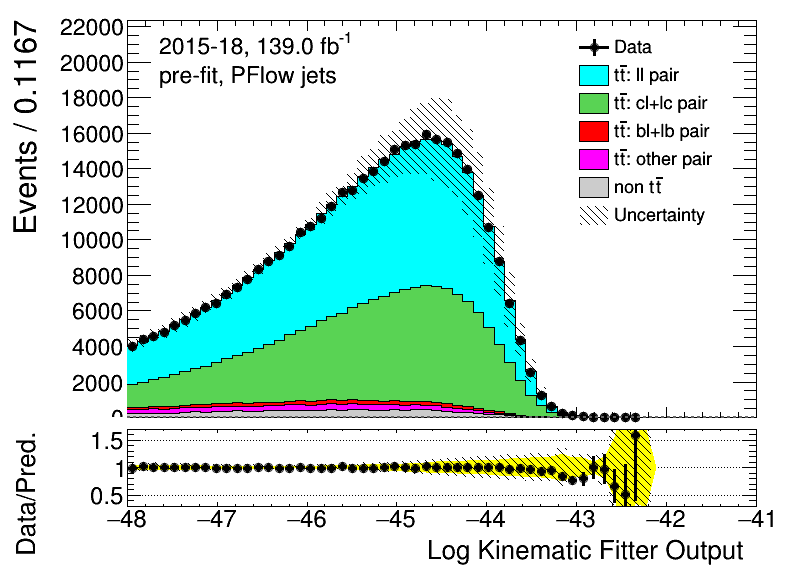
\includegraphics[width=0.45\textwidth]{FTAG_plots/pretagNoRwwithhighpTPFlowall/DataMC_h_LLR.png}
	\caption{Distribution of  the negative logarithm of the likelihood that
	is used to reconstruct the \ttbar\ decay.}
	\label{fig:llr}
\end{figure}
An additional requirement of log-likelihood > -48 is 
placed on the output of the likelihood value for the chosen event permutation. 
An example of the distribution of log-likelihood of the best permutations 
is shown in Figure~\ref{fig:llr}. 
In this figure, the data events are compared against the simulation.
The majority of the events come from \ttbar\ production. There is only
a very small fraction of events, which is denoted as ``non \ttbar''
on the figure, that come from other processes like $W$ or $Z$ production
in association with jets or single-top production.


\section{Event selection}
\label{Event selection}
 % The analysis uses the full available integrated luminosity collected with the ATLAS detector from the all years. This corresponds to a collected luminosity of 139 fb$^{-1}$. The event selection aims to select a sample enriched in $t\bar{t}$ events. The lowest un-prescaled single electron and single-muon triggers are used.
\subsection{Standard selection}
\label{standard selection}
Events are required to contain exactly one trigger-matched 
lepton with $p_{T} > 27$~GeV and exactly four jets with 
$p_{T} > 25$~GeV. Leptons are required to have $p_{T}$ 
above 27~GeV in order to avoid the turn-on curve for the 
single lepton triggers. Events which contain an additional 
lepton with $p_T > 27$~GeV are rejected. 
The events are also required to have $\MET > 20$~GeV, which is 
assumed to be the result of the neutrino from the leptonically 
decaying $W$ boson. The transverse
mass $m_T$ between the lepton and the \MET, is
constrained as follows:
\[ m_T = \sqrt{2 p_T^\ell \MET (1-\cos\Delta\phi)} > 40~\GeV,\]
where $\Delta\phi = \phi(\MET)-\phi(\ell)$ is the azimuthal difference between
the lepton and \MET.
\begin{table}[htb]
	\centering
	\small
	\setlength\tabcolsep{5pt} 
	\newcolumntype{C}{ @{}>{${}}c<{{}$}@{} }
	\begin{tabular}{|r *2{|rCr}| }
	\hline
	& \multicolumn{3}{|c|}{PFlow jets} & \multicolumn{3}{c|}{Track jets} \\
	\hline
	Data          &     227118       &   &              &   218351  &       &         \\  
	\ttbar\       &     235670       &\pm& 200          &   223770  &\pm& 180     \\
	Non \ttbar\   &     7610         &\pm& 120          &   7280    &\pm& 100    \\
	\hline
	Data/MC       &     0.934        &\pm& 0.002        &   0.945   &\pm& 0.002 \\
	\hline
	\end{tabular}
	\vspace{0.2cm}
	\caption{Standard selection: prefit comparison of the  number of events in data and in 
	simulation considering the PFlow jets and the VR-Track jets for 
	events with exactly 4 jets.}
	\label{tab:yields_standard}
\end{table}
\begin{figure}[bth]
	\centering
	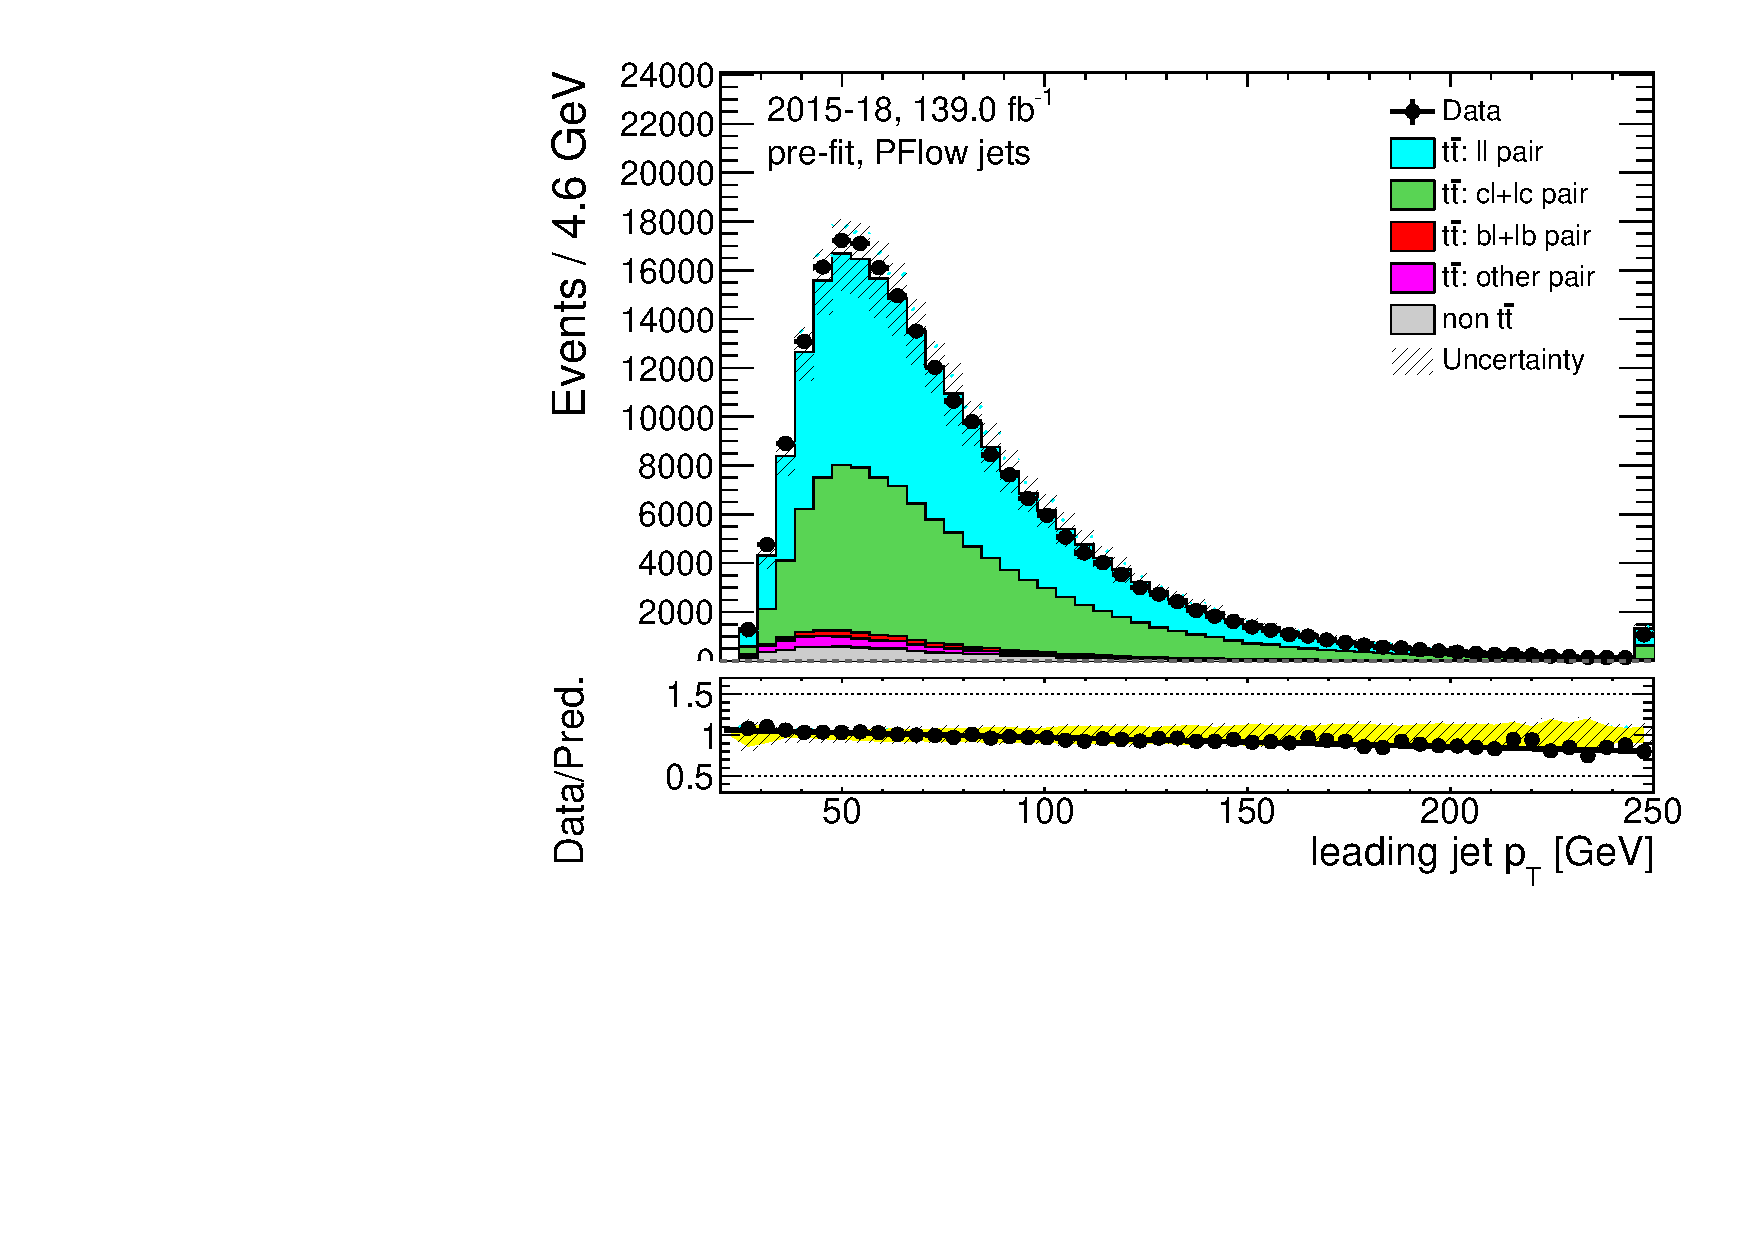
\includegraphics[width=0.45\textwidth]{FTAG_plots/pretagNoRwwithouthighpTPFlowall/DataMC_h_J0_pt.pdf}
	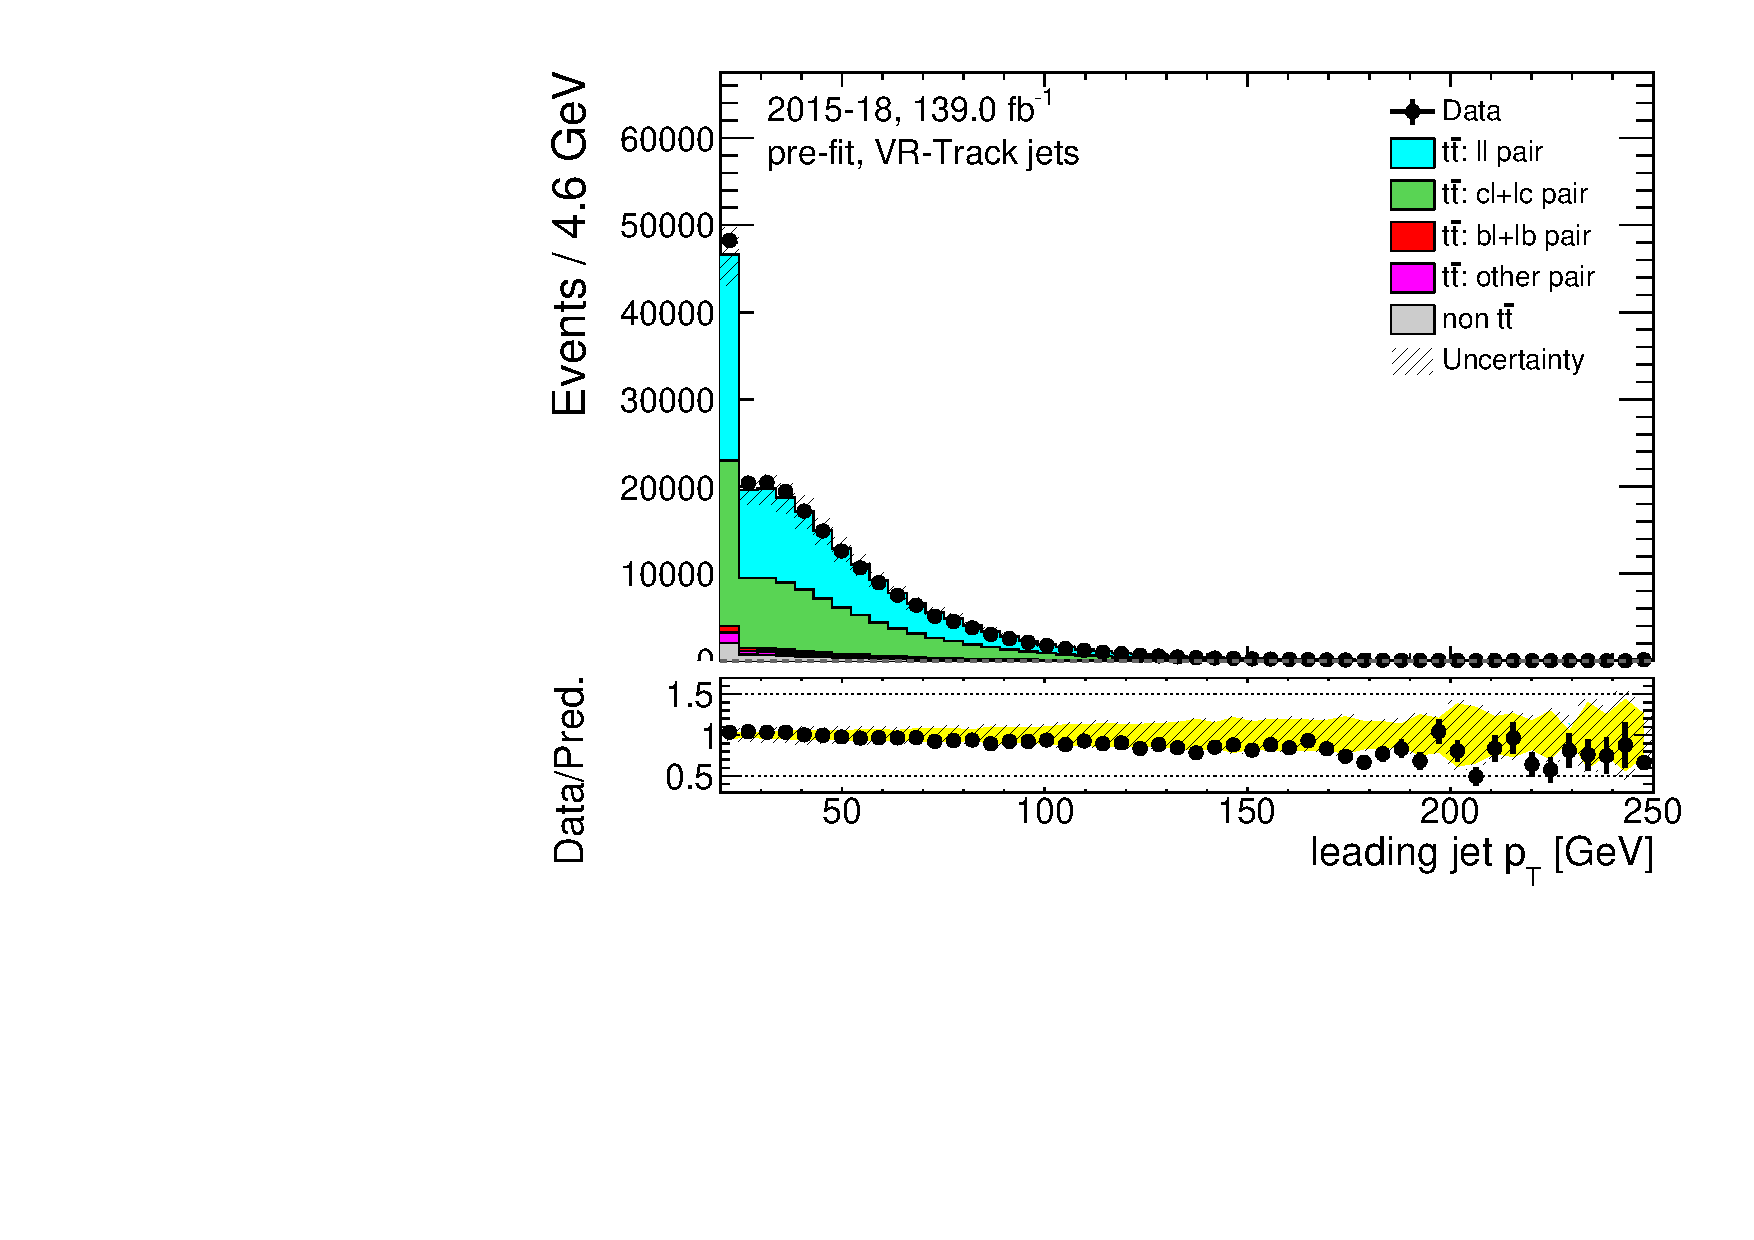
\includegraphics[width=0.45\textwidth]{FTAG_plots/pretagNoRwwithouthighpTVRJetsall/DataMC_h_J0_pttrackjet.pdf}\\
	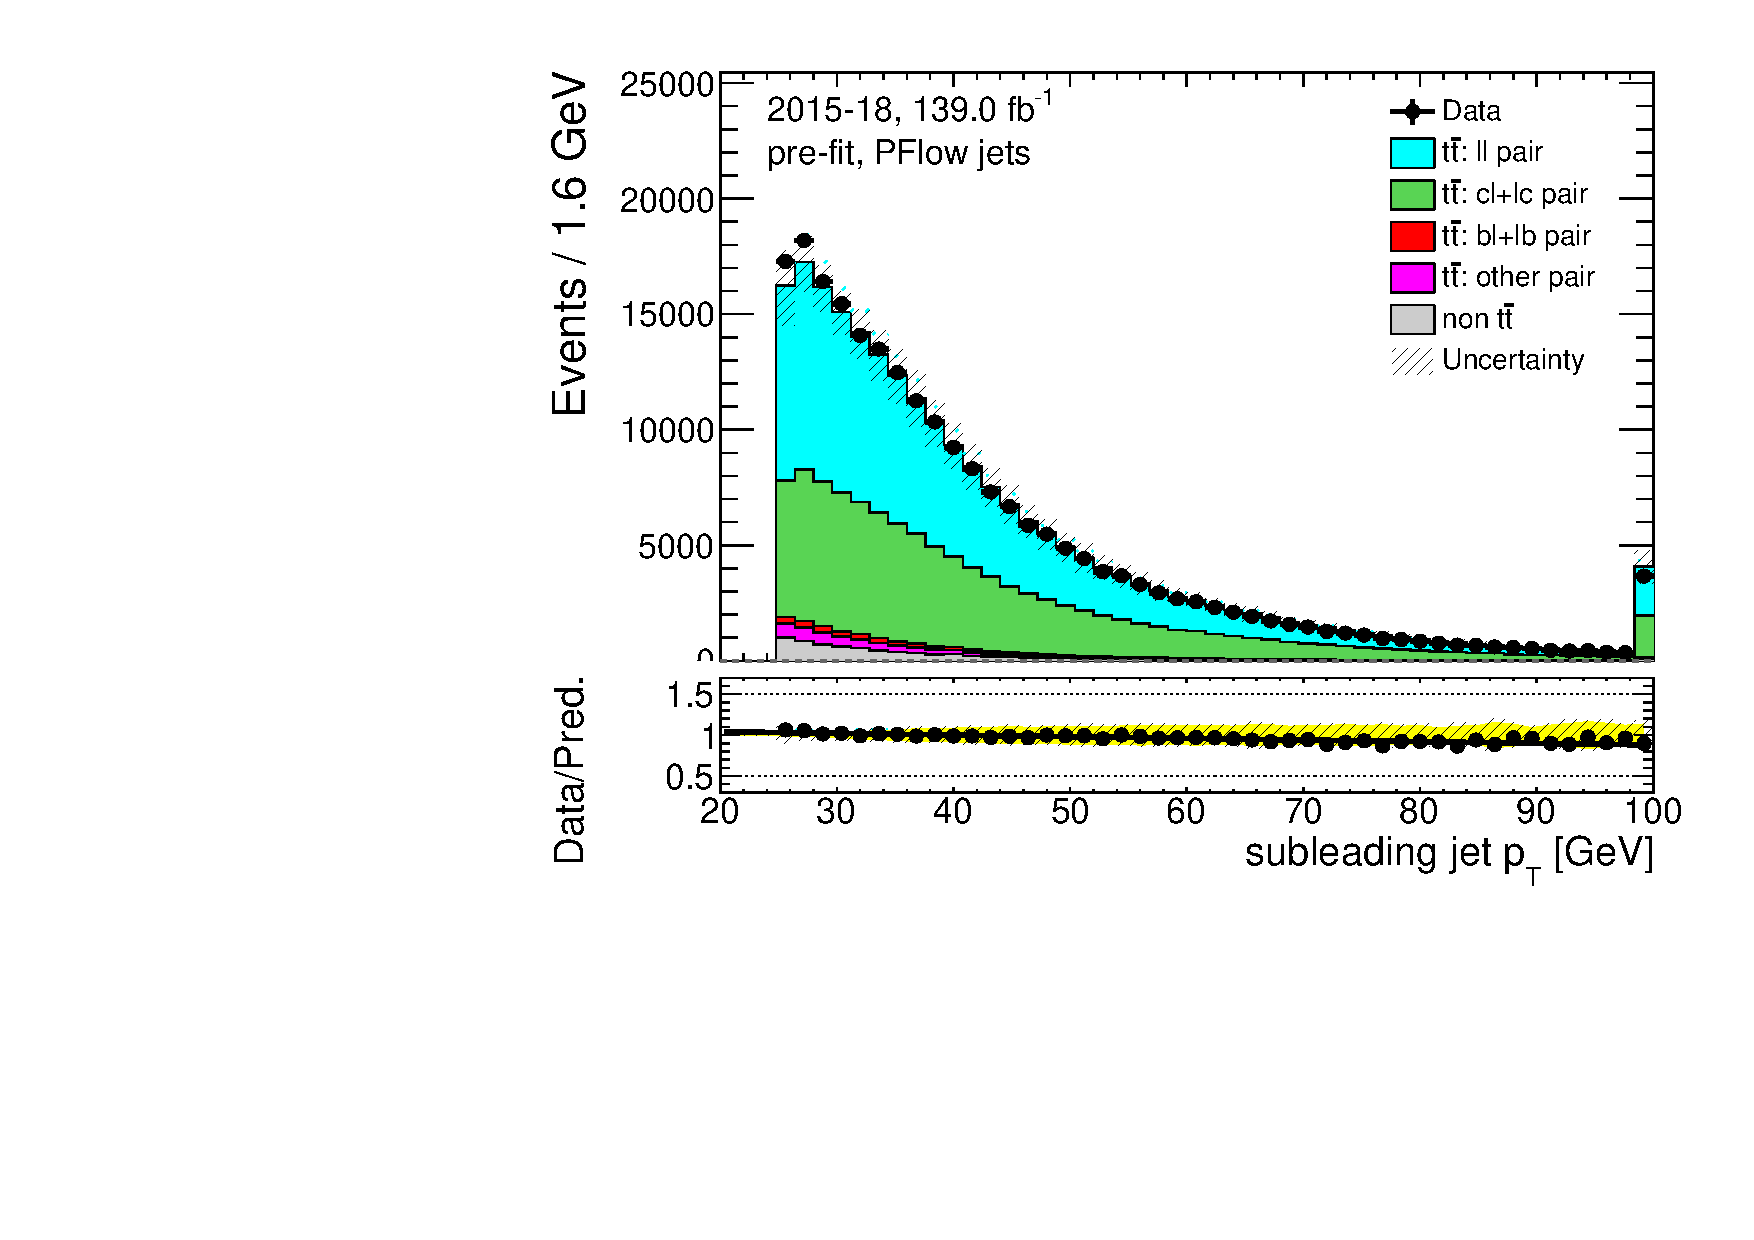
\includegraphics[width=0.45\textwidth]{FTAG_plots/pretagNoRwwithouthighpTPFlowall/DataMC_h_J1_pt.pdf}
	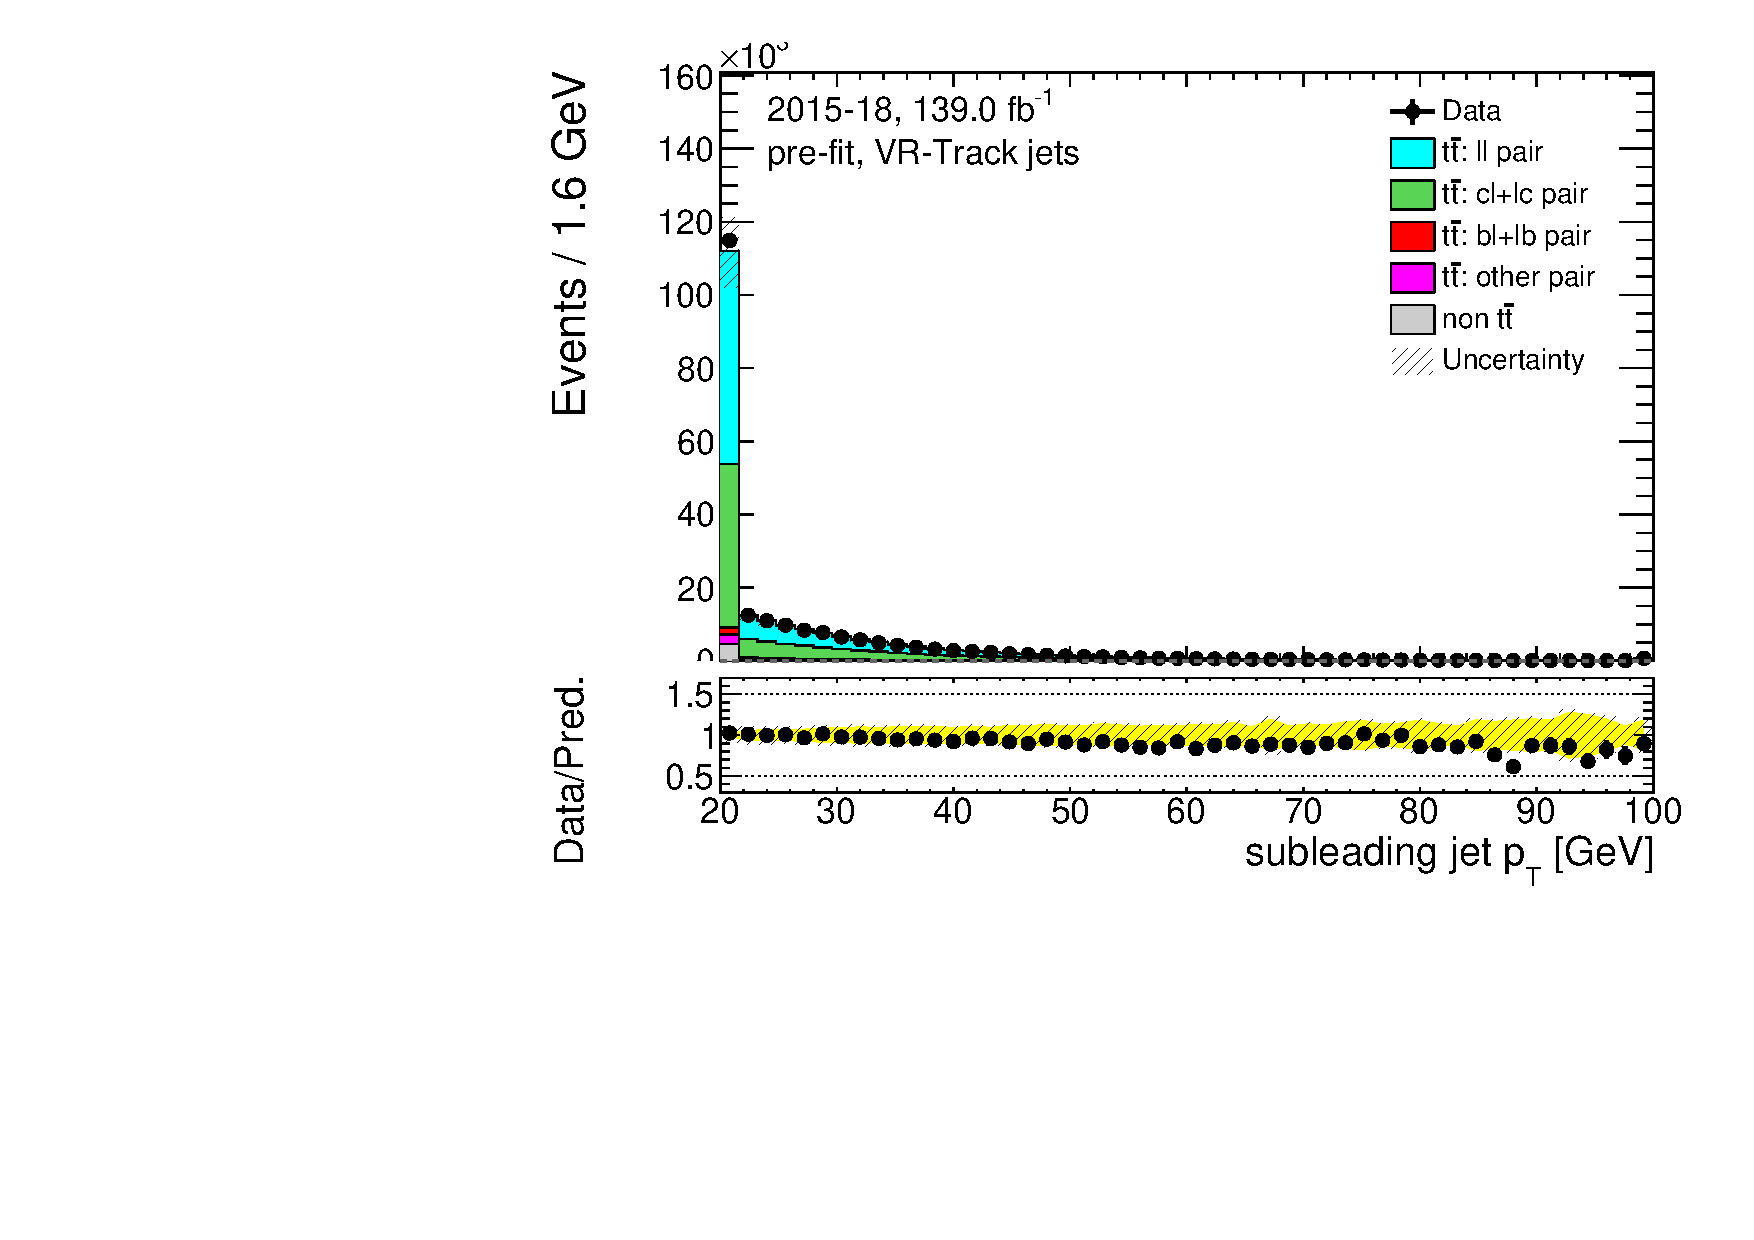
\includegraphics[width=0.45\textwidth]{FTAG_plots/pretagNoRwwithouthighpTVRJetsall/DataMC_h_J1_pttrackjet.pdf}\\
	\caption{Standard selection: data versus simulation of the leading and sub-leading $W$ jet \pt\ 
	for the PFlow jets in the left column and for VR-Track jets in the right column. 
	The leading jet and sub-leading jet refer to the highest \pt\ $W$ jet and the 
	second highest \pt\ jet, respectively. The 'non \ttbar' background 
	indicates background comes from non-\ttbar\ processes like $W$ or $Z$ production
	in association with jets or single-top production.
	The error in the table (and the following yields tables for
	different selection) is stats-only. }
	\label{fig:kinematic_distributions_standard}
\end{figure}
% Due to the requirement on jet $p_T$ and binning strategy, the calibration 
% result can be applied to jets with $p_{T}$ between 25 to 200~GeV. 
The yields of the data and the MC are given in Table \ref{tab:yields_standard}.
An example of the \pt\ distributions
before any tagging or fitting and 
after the standard selection is shown in Figure~\ref{fig:kinematic_distributions_standard}. 
More plots can be found in Appendix \ref{sec:appendix_standard_selection}.
The yellow band in the lower pad shows the overall systematic uncertainties, combining the 
experimental uncertainties and the \ttbar\ modelling uncertainties, as described in 
Section \ref{sec:FTAG_systematics}. The data/MC ratio shows good agreement 
within the systematic uncertainties. 

\subsection{Low-\pt\ selection}
\label{sec:lowpT_selection}
The author has developed an othorgonal selection to 
extend the calibration in the low-$p_{T}$ region so that the calibration 
can be applied to PFlow jets with $20< \pt\ < 25$~GeV.
The \pt\ threshold of the VR-Track jets is $10$~GeV 
therefore the low-\pt\ selection is not needed. 
Instead of requiring events to 
have exactly 4 jets $\pt\ > 25$~GeV, events are required to have exactly 3 jets with $p_{T} > 25$~GeV 
and exactly 1 jet with $25$~GeV $> p_{T} > 20$~GeV. Other than that, 
all requirements for the selection are the same. 
This additional cut provides candidates for the PFlow $W$ jet that is used 
for calibration in the $20-25$~GeV region. 
The inclusive yields of the low-\pt\ selection 
of the data and the MC are given in Table \ref{tab:yields_lowpT}, and
the \pt\ distributions of the $W$ jets are shown in Figure~\ref{fig:kinematic_distributions_lowpT}.
More plots of the kinematic distributions
are shown in Appendix \ref{sec:appendix_lowpT_selection}. 
Good agreement between MC and data 
is shown in these distributions, and the $p_{T}$ range of the sub-leading has gone down to 20~GeV. 


\begin{table}[bht]
	\centering
	\small
	\setlength\tabcolsep{5pt} 
	\newcolumntype{C}{ @{}>{${}}c<{{}$}@{} }
	\begin{tabular}{|r *1{|rCr}| }
	\hline
	& \multicolumn{3}{|c|}{PFlow jets} \\
	\hline
	Data          &     59987       &   &                      \\  
	\ttbar\       &     56530       &\pm&     90        		 \\
	Non \ttbar\   &     3340        &\pm&     60    		 \\
	\hline
	Data/MC       &     1.002       &\pm&  0.004      			 \\
	\hline
	\end{tabular}
	\vspace{0.2cm}
	\caption{Low-\pt\ selection: prefit comparison 
	of the number of events in data and MC 
	for the PFlow $W$ jets. Events are required to have 
	exactly 3 jets with $\pt\ > 25$~GeV 
	and one jet with $20 < \pt\ < 25$~GeV.}
	\label{tab:yields_lowpT}
\end{table}

\begin{figure}[H]
	\centering
	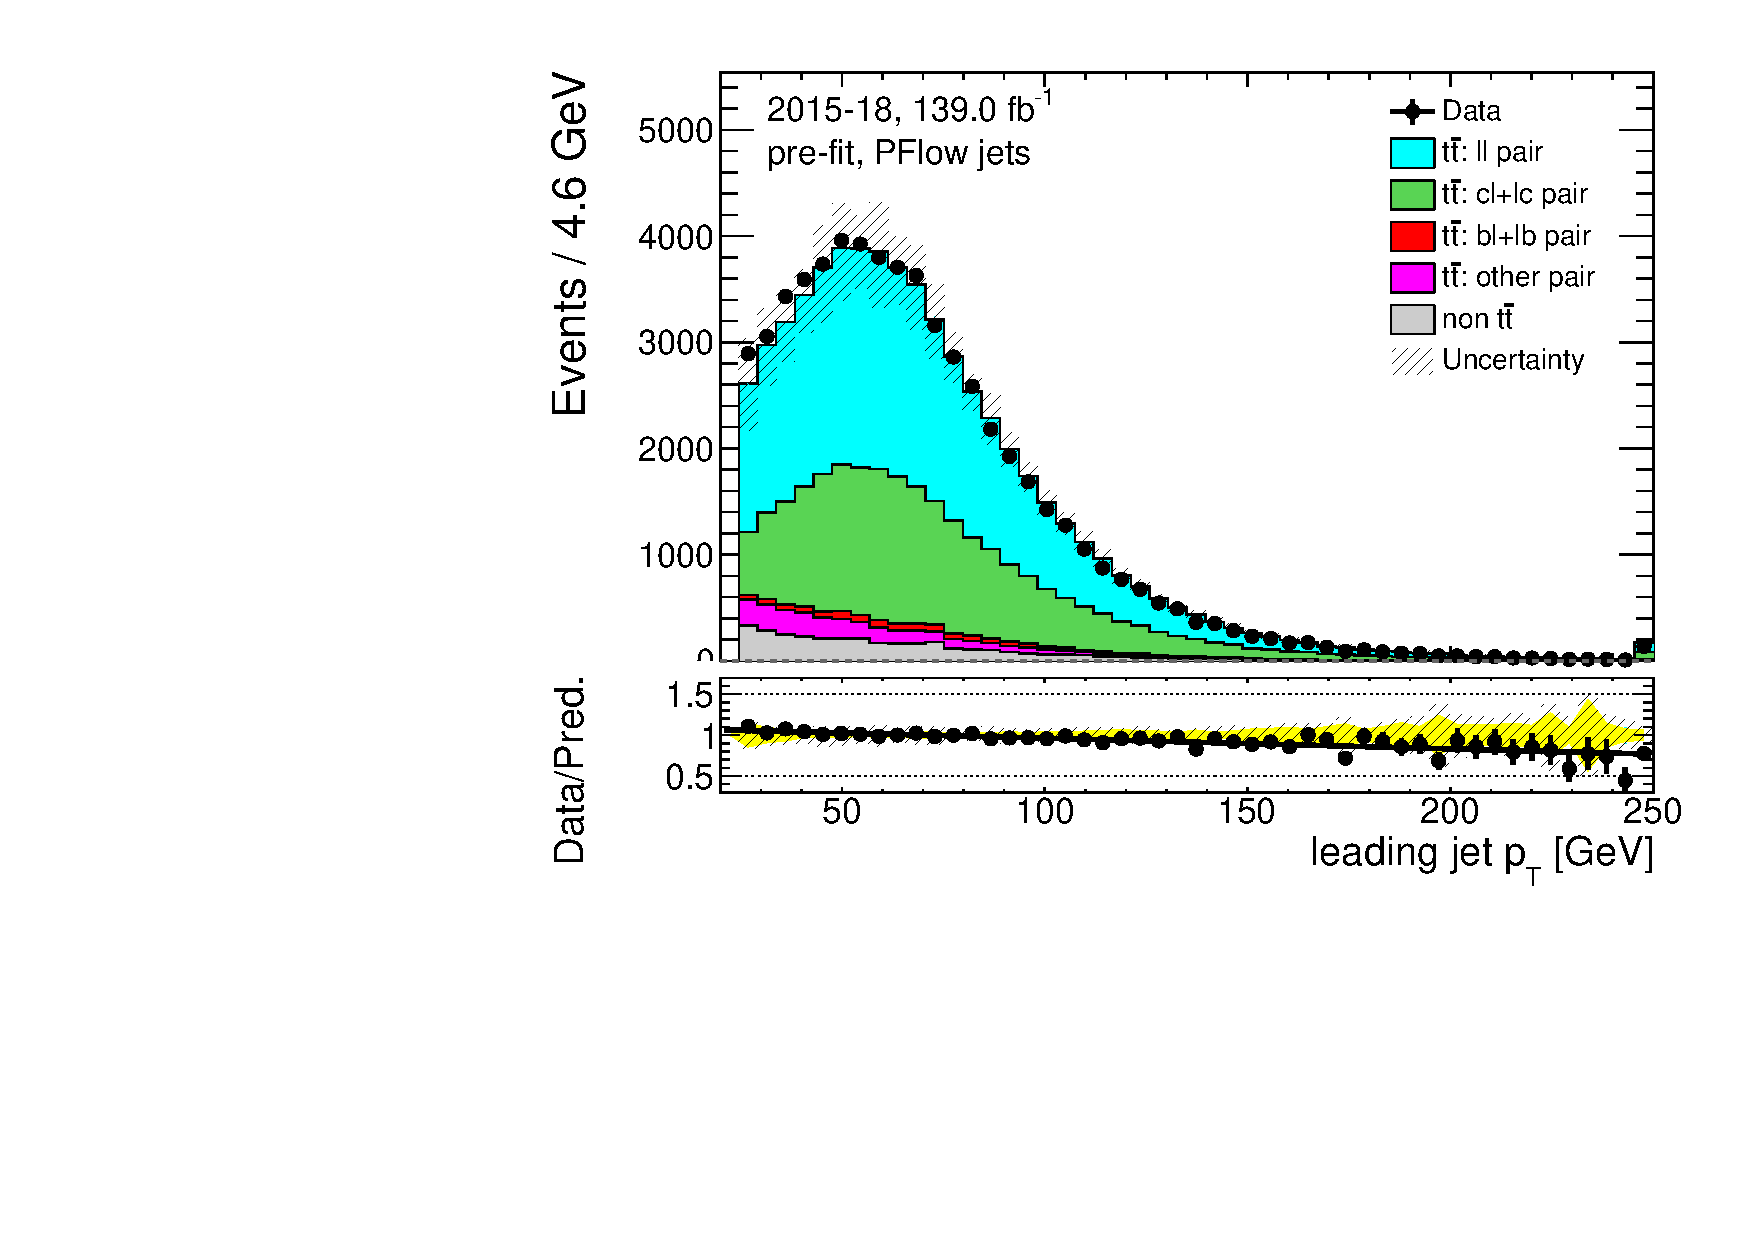
\includegraphics[width=0.45\textwidth]{FTAG_plots/pretagNoRwLowpTPFlowall/DataMC_h_J0_pt.pdf}
	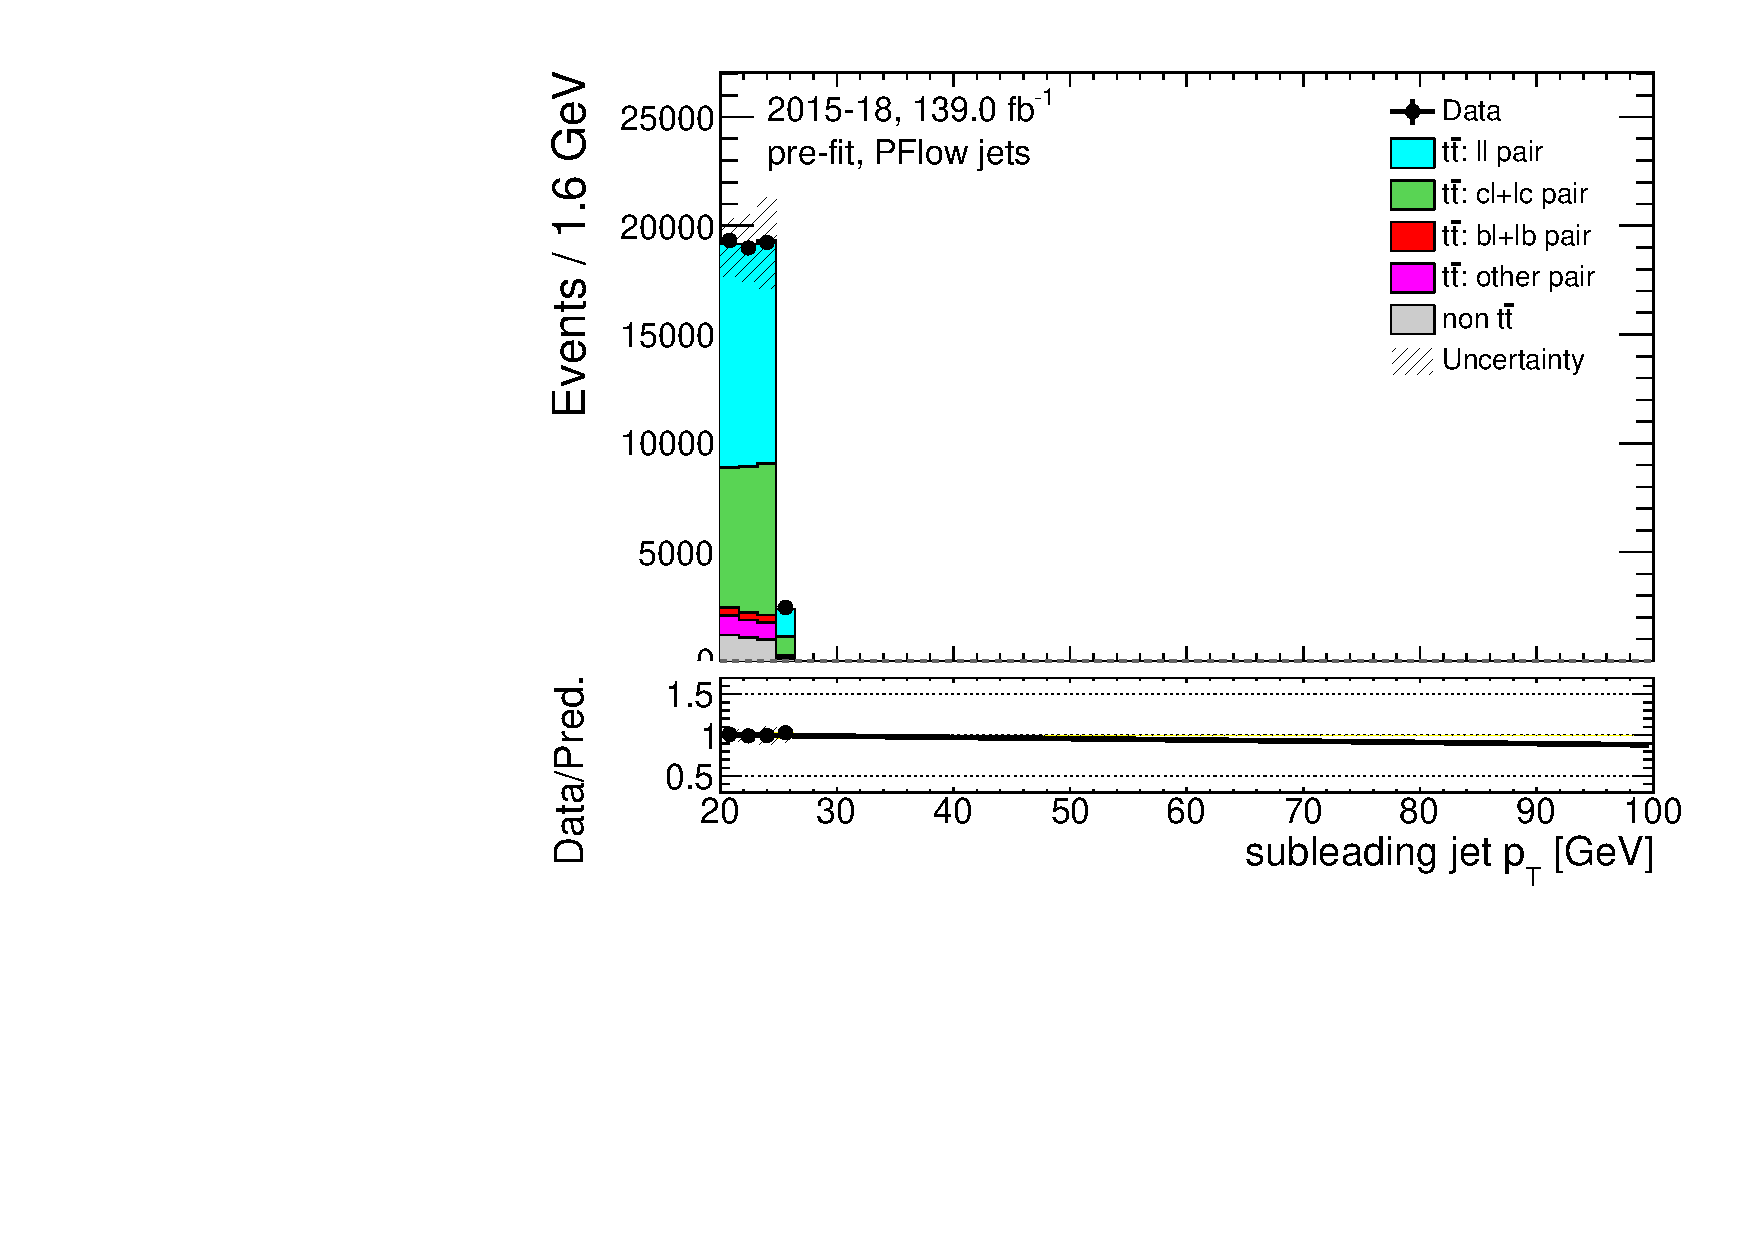
\includegraphics[width=0.45\textwidth]{FTAG_plots/pretagNoRwLowpTPFlowall/DataMC_h_J1_pt.pdf}\\
	\caption{Low-\pt\ selection: data versus simulation of the 
	PFlow $W$ jets \pt. }
	\label{fig:kinematic_distributions_lowpT}
\end{figure}


\subsection{High-$p_T$ selection}
\label{high_pt_selection}
It has been observed that in the previous calibrations that the statistics 
are relatively low for the high-\pt\ region (e.g.\ jet $\pt\ > 100$~GeV). 
Therefore, the author has worked on an othorgonal selection to improve this situation.
Instead of requiring events to have exactly 4 jets, events are required to 
have at least 5 jets with $p_{T} > 25$~GeV, in which at least 
1 jet with $\pt\ > 70$~GeV. Other than that, all 
requirements for the selection remain the same. 


The choice of cut value at $70$~GeV is based on the
study shown in the following. 
The effect on the \cjet\ purity and the potential statistical gain is investigated, 
where the \cjet\ purity is defined as:
\begin{equation}
\cjetineq\ \rm{purity} = \frac{N_{\rm{true}\ \cjetunder}}{N_{\rm{all}}},
\end{equation}
where $N_{\rm{true}\ \cjetunder}$ stands for the number of events with a 
true \cjet\ from the $W$ decay, and $N_{\rm{all}}$ stands for the number of all events. 
The ideal situation is the high-\pt\ selection will maximally increase the 
statistics while mininally decreasing the \cjet\ purity, therefore a figure of merit $P^{\rm{Cut}}$
is defined as:
\[P^{\rm{Cut}} = \frac{\sum_i{\rm{Gain\ in\ stats}^2_i}}{\sum_i{\cjetineq \rm{purity}^2_i }}, \]
where i stands for the number of bins. The ``Gain in stats'' stands for increase in 
statistics and it's summed over all bins in Figure~\ref{fig:cutvalue}.
The \cjet\ purity and the statistical gain are calculated for 4 different cut 
values as shown in Figure~\ref{fig:cutvalue}, comparing with the cut value of 0. 
The value of $70$~GeV is chosen as it gives the highest value of $P^{\rm{Cut}}$. 


\begin{figure}[bth]
	\centering
	\begin{subfigure}[t]{.38\linewidth}
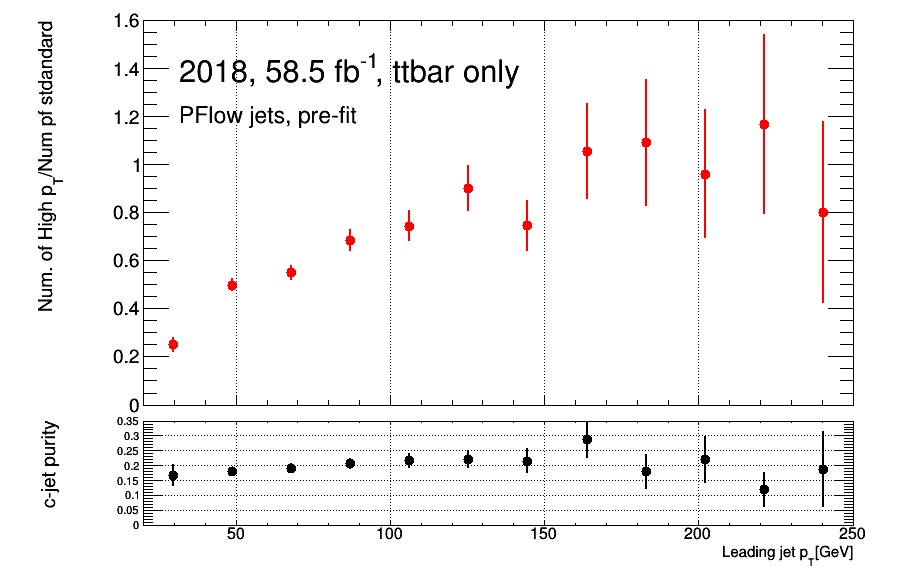
\includegraphics[width=1\textwidth]{FTAG_plots/stat_gains/statsgain_0GeV.png}
\caption{No cut}
\end{subfigure}
\begin{subfigure}[t]{.38\linewidth}
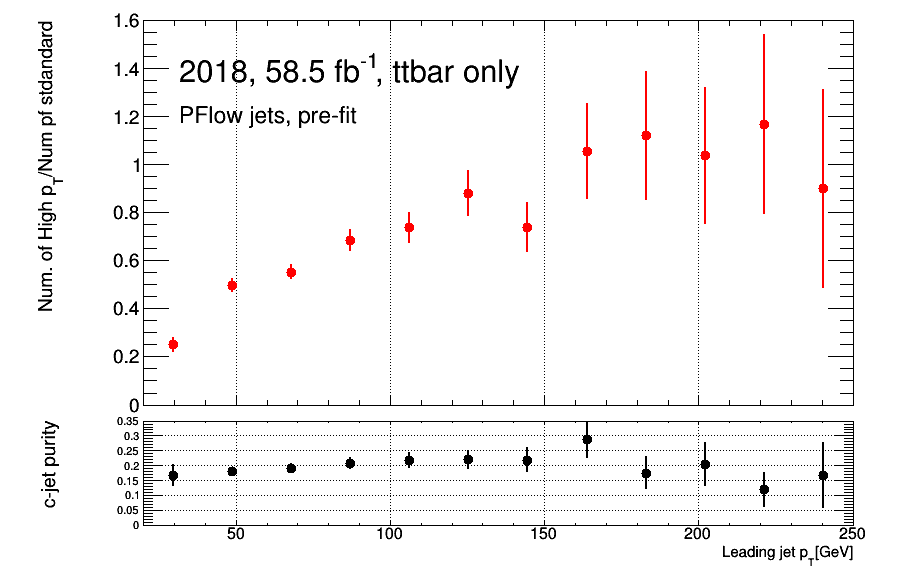
\includegraphics[width=1\textwidth]{FTAG_plots/stat_gains/statsgain_40GeV.png}
\caption{Cut value: 40~GeV}
\end{subfigure}
\begin{subfigure}[t]{.38\linewidth}
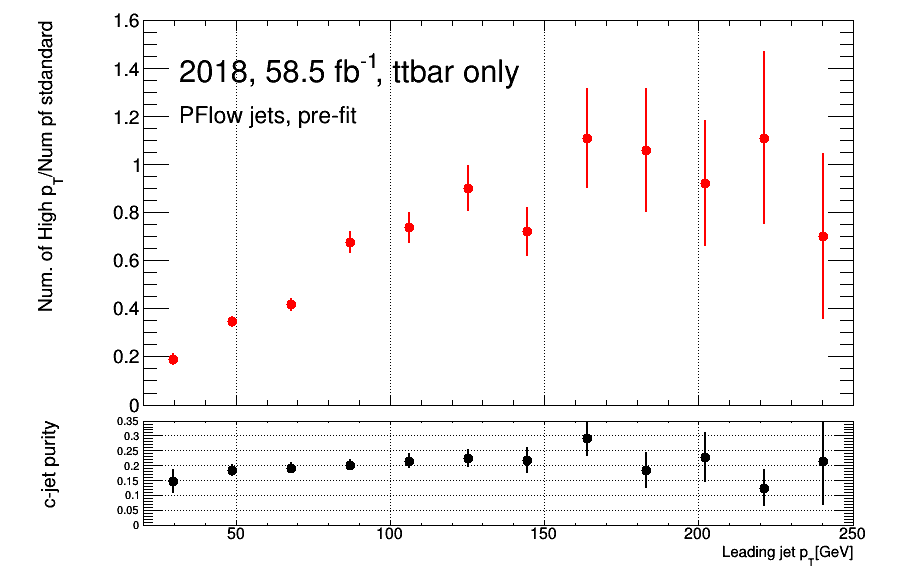
\includegraphics[width=1\textwidth]{FTAG_plots/stat_gains/statsgain_70GeV.png}
\caption{Cut value: 70~GeV}
\end{subfigure}
\begin{subfigure}[t]{.38\linewidth}
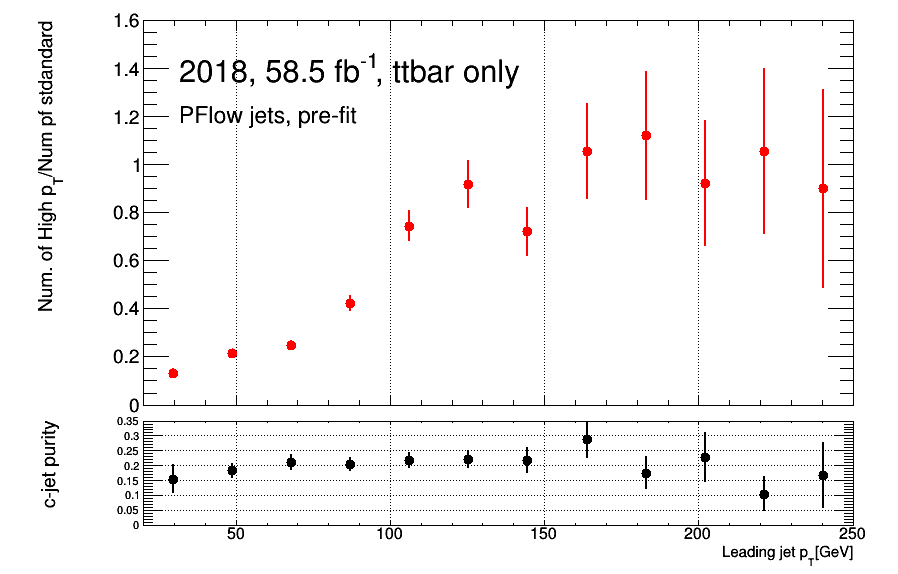
\includegraphics[width=1\textwidth]{FTAG_plots/stat_gains/statsgain_90GeV.png}
\caption{Cut value: 90~GeV}
\end{subfigure}
\begin{subfigure}[t]{.38\linewidth}
\centering
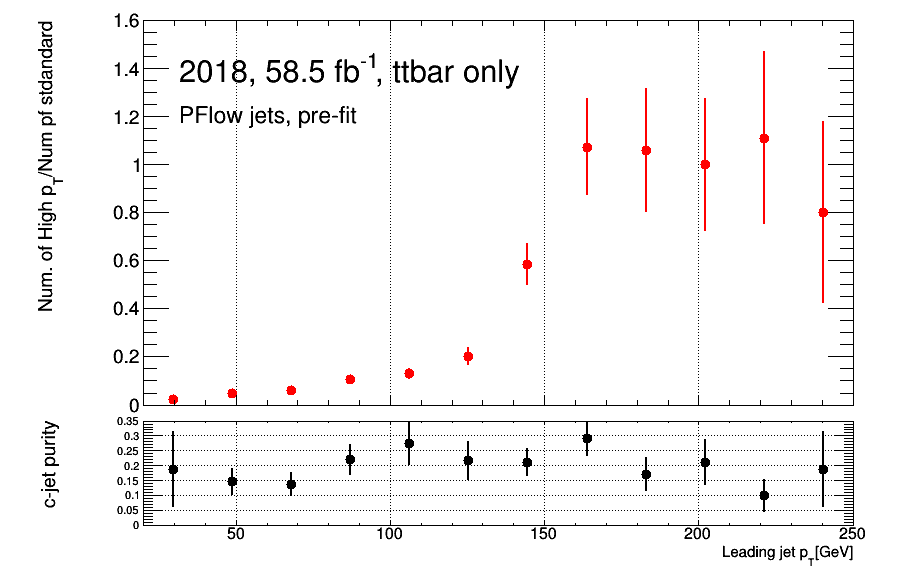
\includegraphics[width=1\textwidth]{FTAG_plots/stat_gains/statsgain_140GeV.png}
\caption{Cut value: 140~GeV}
\end{subfigure}

\caption{Comparison of different cut values in terms of gain in stats and \cjet\ purity.}
\label{fig:cutvalue}
\end{figure}

\begin{table}[ht]
	\centering
	\small
	\setlength\tabcolsep{5pt} 
	\newcolumntype{C}{ @{}>{${}}c<{{}$}@{} }
	\begin{tabular}{|r *2{|rCr}| }
	\hline
	& \multicolumn{3}{|c|}{PFlow jets} & \multicolumn{3}{c|}{Track jets} \\
	\hline
	
	Data    &     98273  &           &   &        83957   &              &   \\ 
	\ttbar\ &    99430 &\pm&  120 &        87476 &\pm&  110     \\
	Non \ttbar\   &      1842  &\pm&  21 &          1570  &\pm&  20     \\
	\hline
	Data/MC &      0.97  &\pm&  0.003   &     0.94  &\pm&  0.003       \\
	\hline

	\end{tabular}
	\vspace{0.2cm}
	\caption{High-\pt\ selection: prefit comparison of the number of events in data and in 
	simulation considering the PFlow $W$ jets and the VR-Track jets.}
	\label{tab:yields_highpT}
	\end{table}

\begin{figure}[bth]
	\centering
	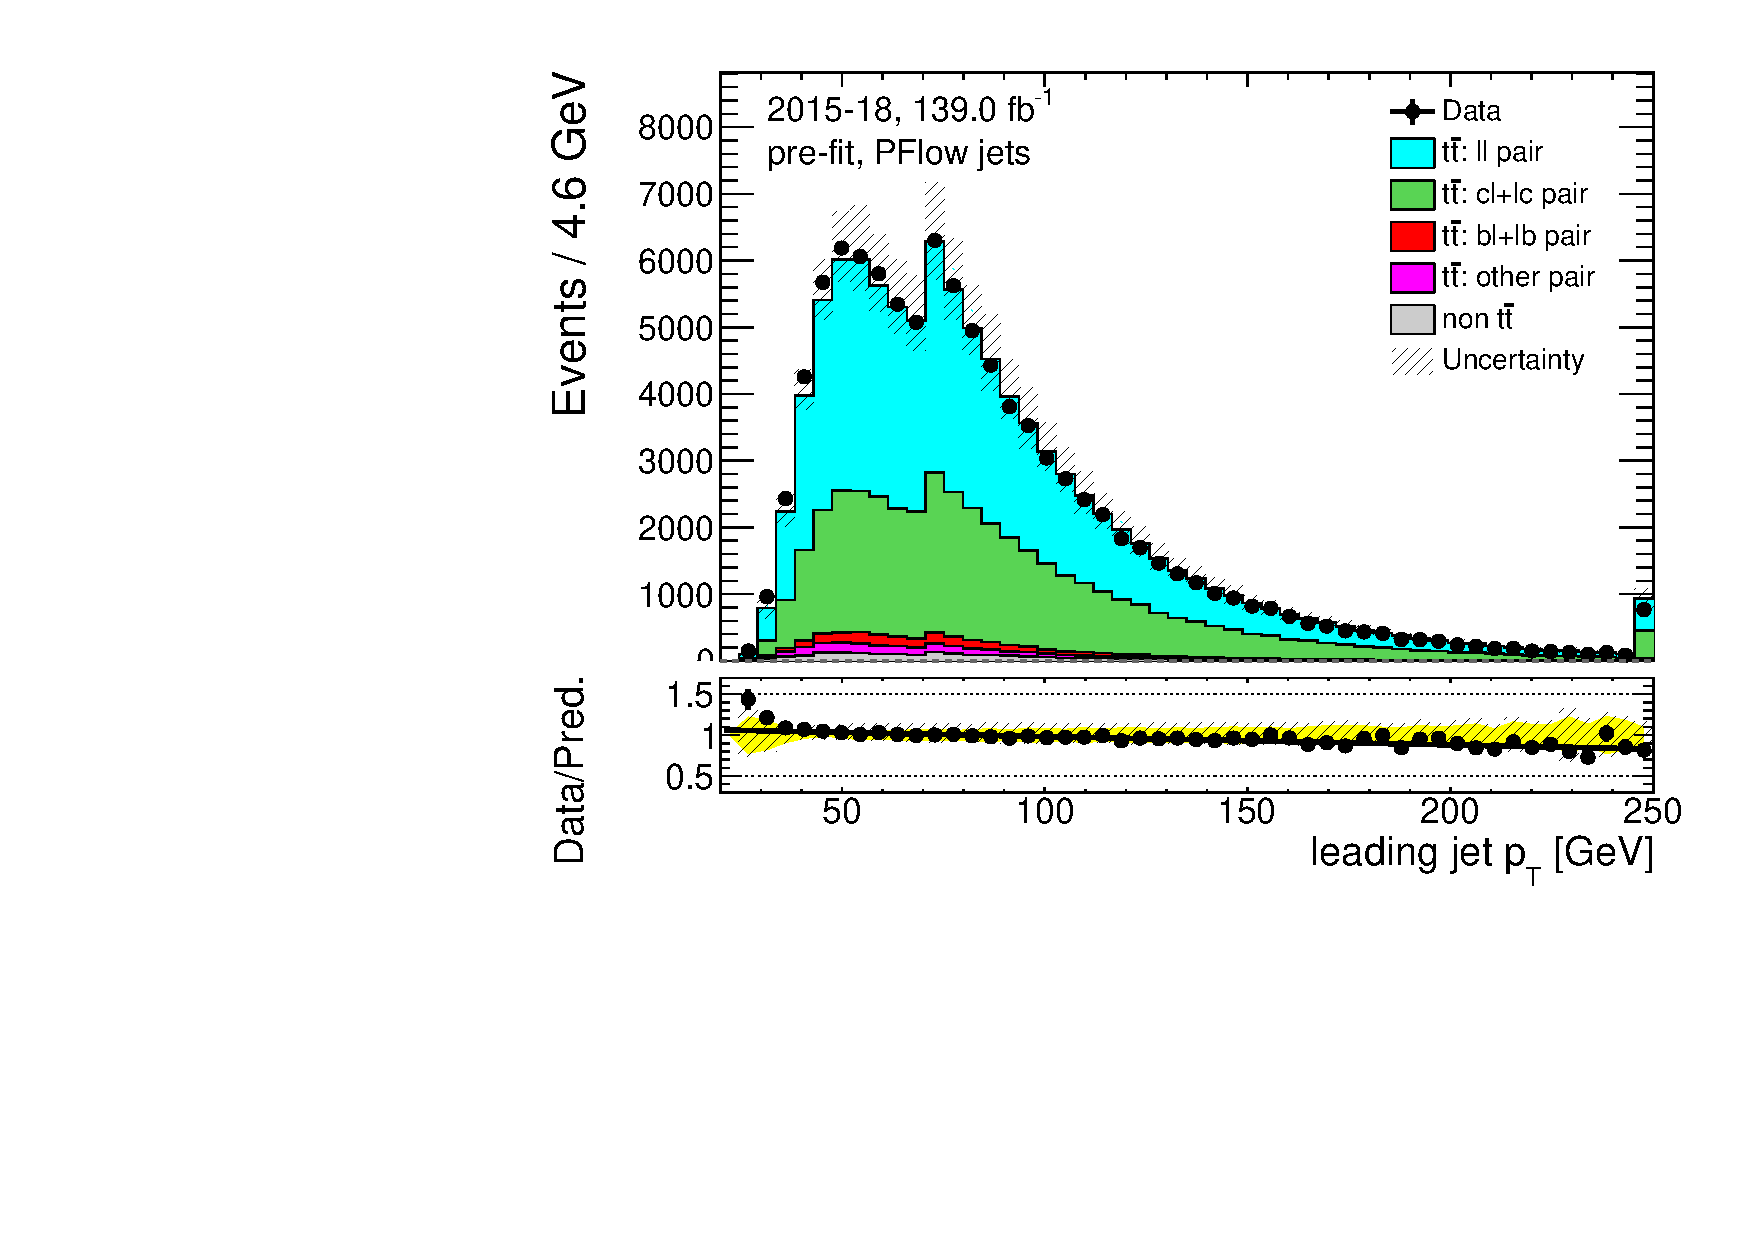
\includegraphics[width=0.45\textwidth]{FTAG_plots/pretagNoRwnewonlyPFlowall/DataMC_h_J0_pt.pdf}
	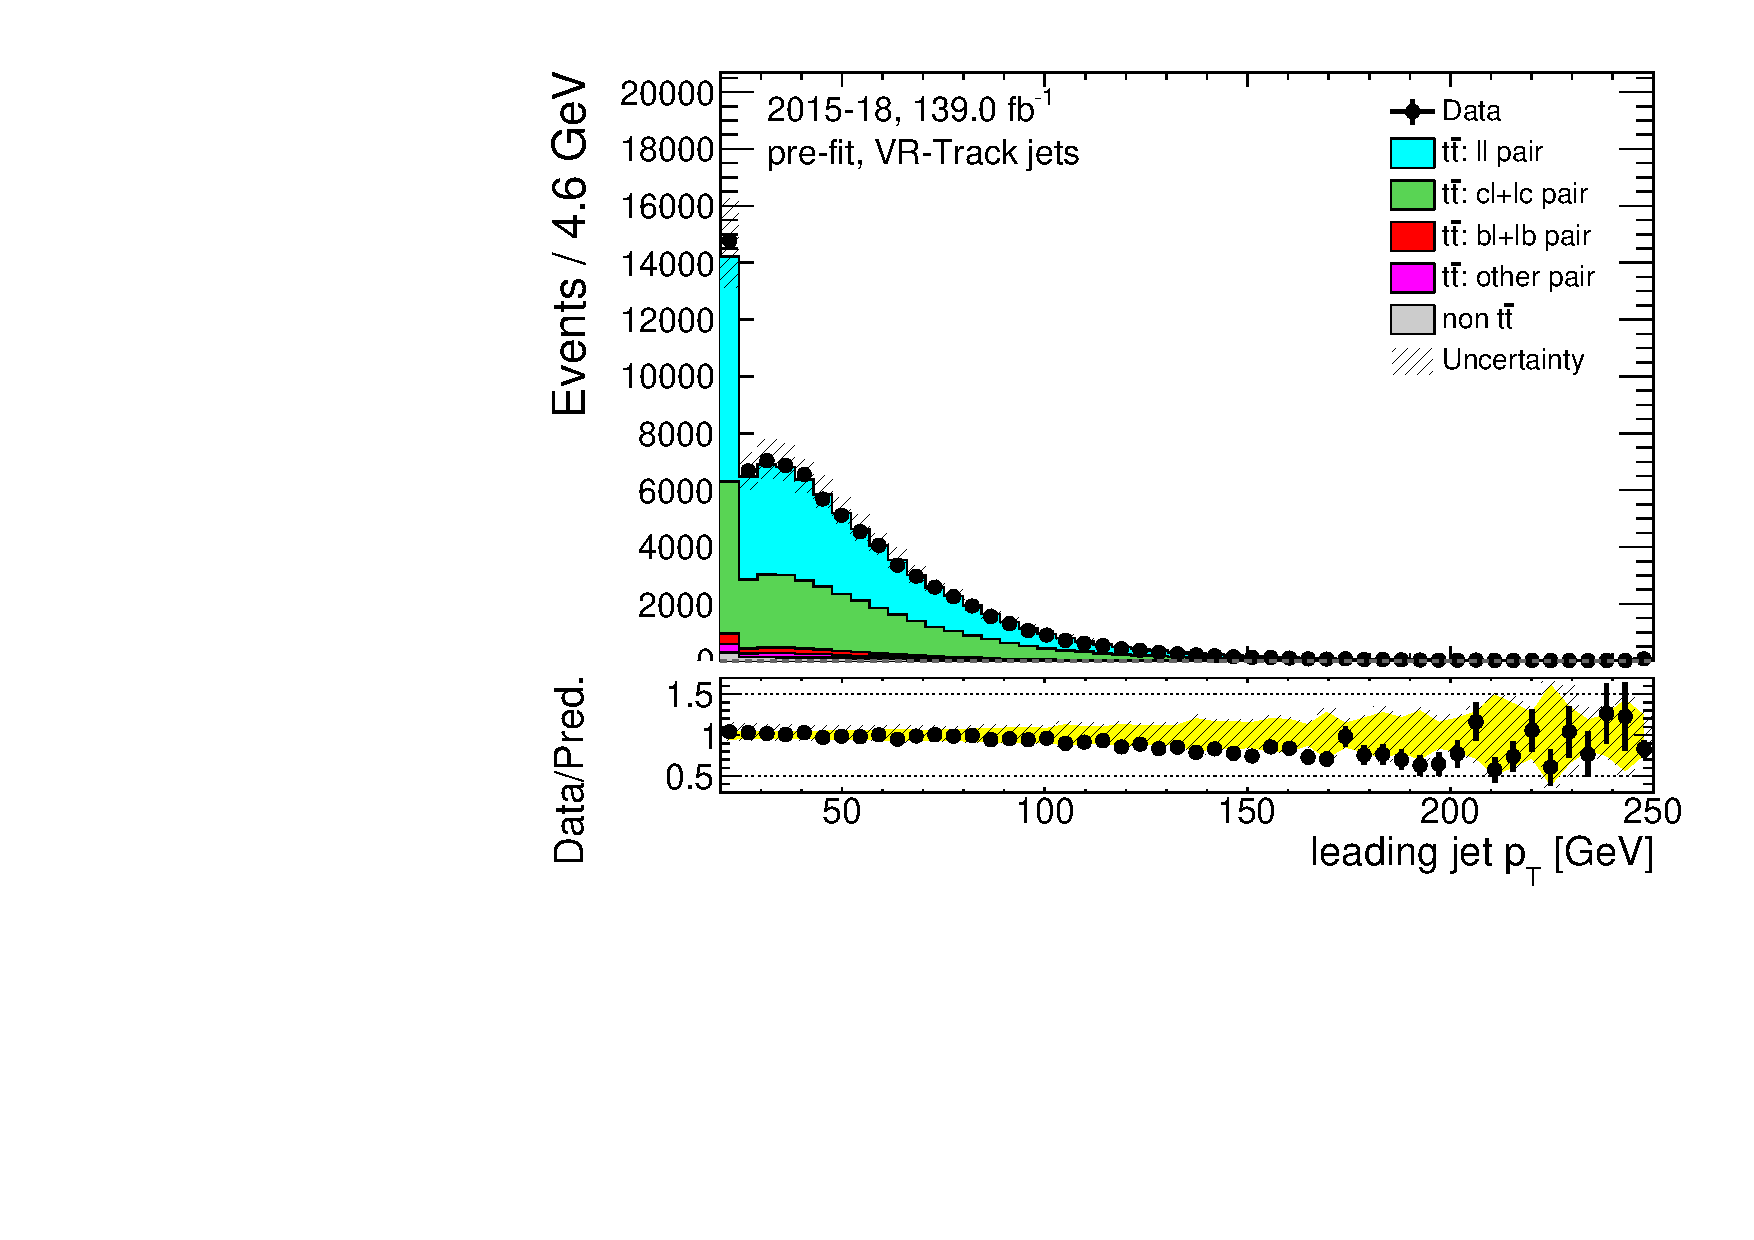
\includegraphics[width=0.45\textwidth]{FTAG_plots/pretagNoRwnewonlyVRJetsall/DataMC_h_J0_pttrackjet.pdf}\\
	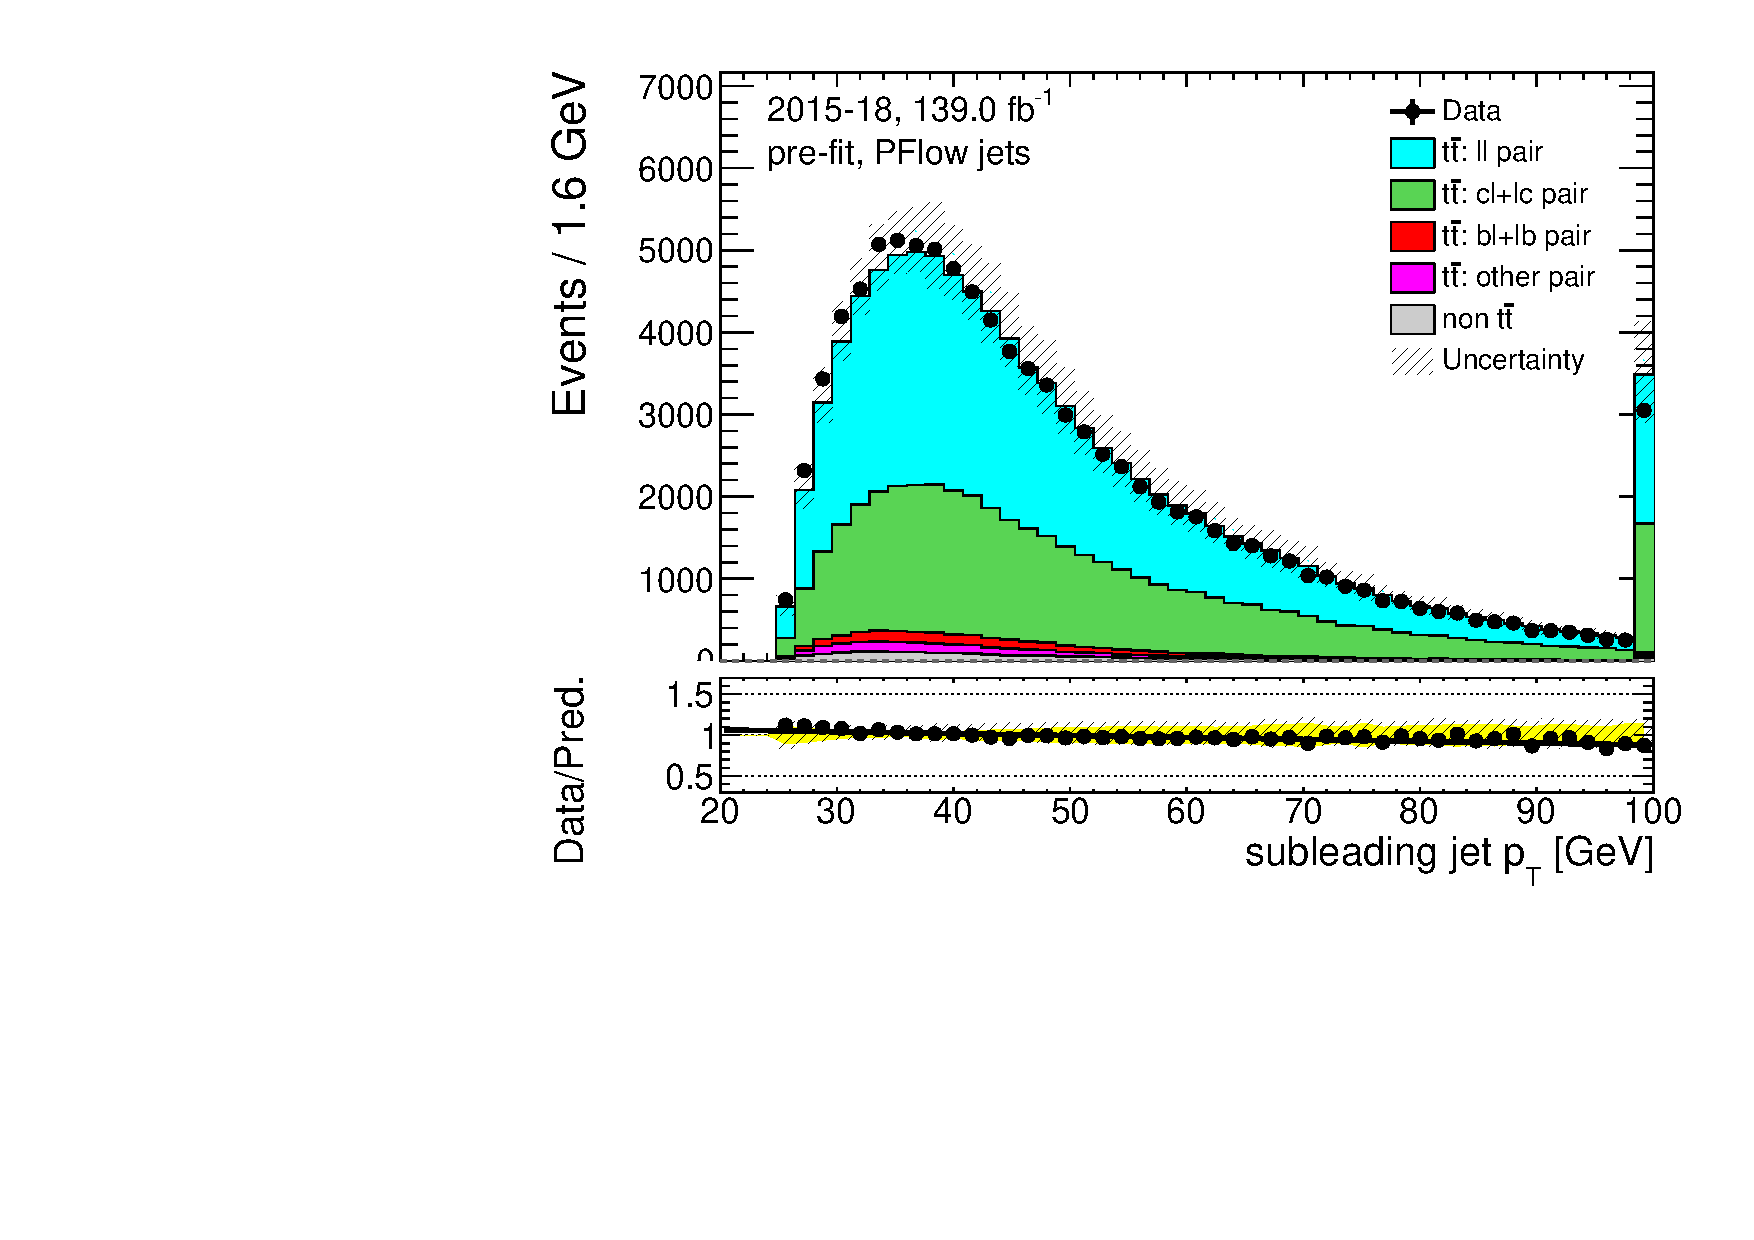
\includegraphics[width=0.45\textwidth]{FTAG_plots/pretagNoRwnewonlyPFlowall/DataMC_h_J1_pt.pdf}
	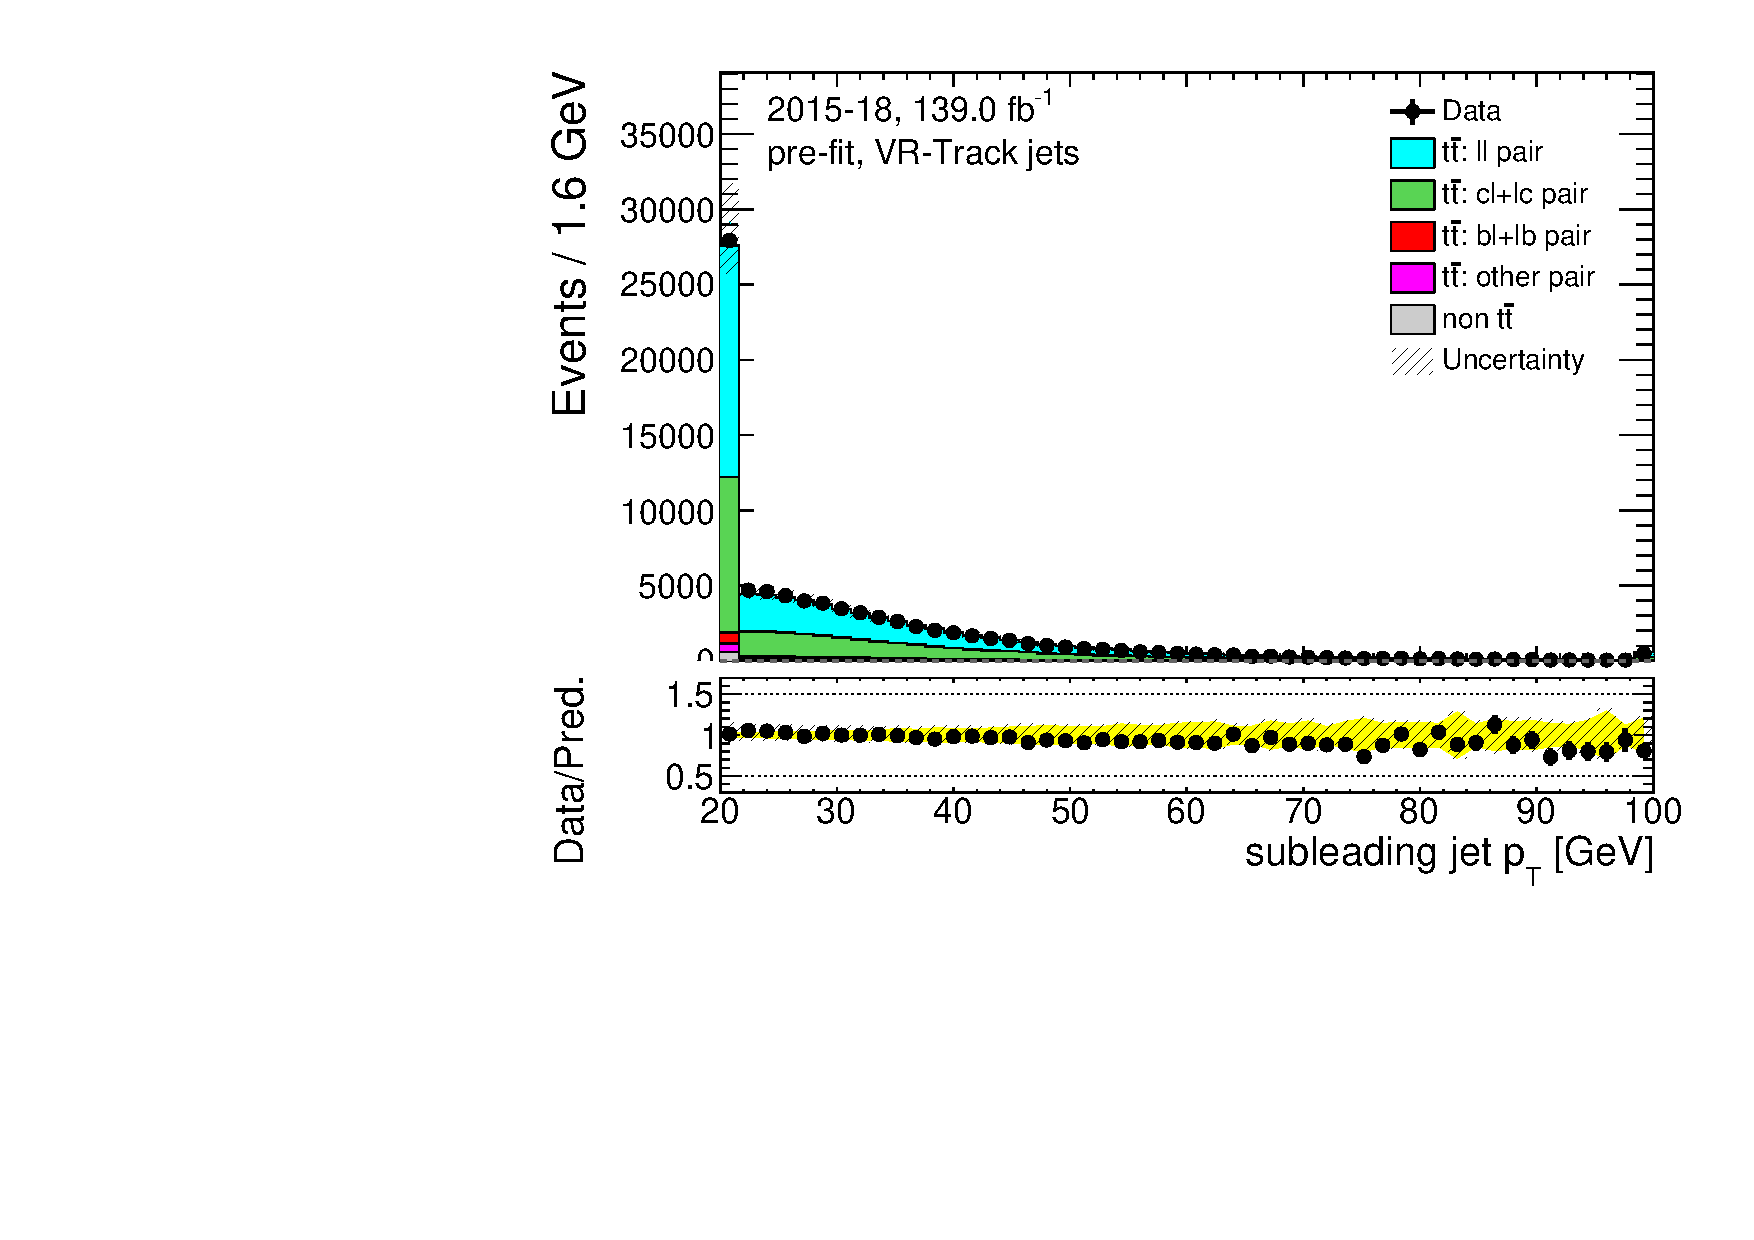
\includegraphics[width=0.45\textwidth]{FTAG_plots/pretagNoRwnewonlyVRJetsall/DataMC_h_J1_pttrackjet.pdf}\\
	\caption{High-\pt\ selection: data versus simulation of $W$ jets \pt\ for 
	PFlow jets in the left column and for VR-Track jets in the right column.}
	\label{fig:kinematic_distributions_highpT}
\end{figure}
	

The yields of the data and the MC are given in Table \ref{tab:yields_highpT}. 
An example of the \pt\ distributions before any tagging or fitting, applying 
the high-\pt\ selection is shown in Figure~\ref{fig:kinematic_distributions_highpT}. 
In general the event statistics improve about 80\% in region with \pt\ > 70~GeV as desired.
More plots can be found in Appendix \ref{sec:appendix_highpT_selection}.




\subsection{Combined selection}
\label{combined_selection}
As the standard selections, low-\pt\ selection and high-\pt\ selection are othorgonal 
to each other, all the selections are combined to provide the maximum range 
and statistics for the calibration. 
The yields of the data and the MC are given in Table \ref{tab:yields_combined}, 
an example of the \pt\ distributions before any tagging or fitting and 
after the combined selection is shown in Figure~\ref{fig:kinematic_distributions_combined}. More plots 
can be found in Appendix \ref{sec:appendix_combined_selection}.

\begin{table}[ht]
	\centering
	\small
	\setlength\tabcolsep{5pt} 
	\newcolumntype{C}{ @{}>{${}}c<{{}$}@{} }
	\begin{tabular}{|r *2{|rCr}| }
	\hline
	& \multicolumn{3}{|c|}{PFlow jets} & \multicolumn{3}{c|}{Track jets} \\
	\hline
	Data          &    385378           &      &        &   302308         &  &     \\  
	\ttbar\       &      383520   &\pm&  230 &            302690 &\pm&  200   \\
	Non \ttbar\         &        12420  &\pm&  120 &             8570  &\pm&  100     \\
	Data/MC       &        0.973  &\pm&  0.002 &           0.971 &\pm&  0.002          \\
	\hline

	\end{tabular}
	\vspace{0.2cm}
	\caption{Combined selection: prefit comparison of the number of events in data and in 
	simulation considering the PFlow jets and the VR-Track jets for an inclusive
	selection.}
	\label{tab:yields_combined}
	\end{table}

\begin{figure}[bth]
		\centering
		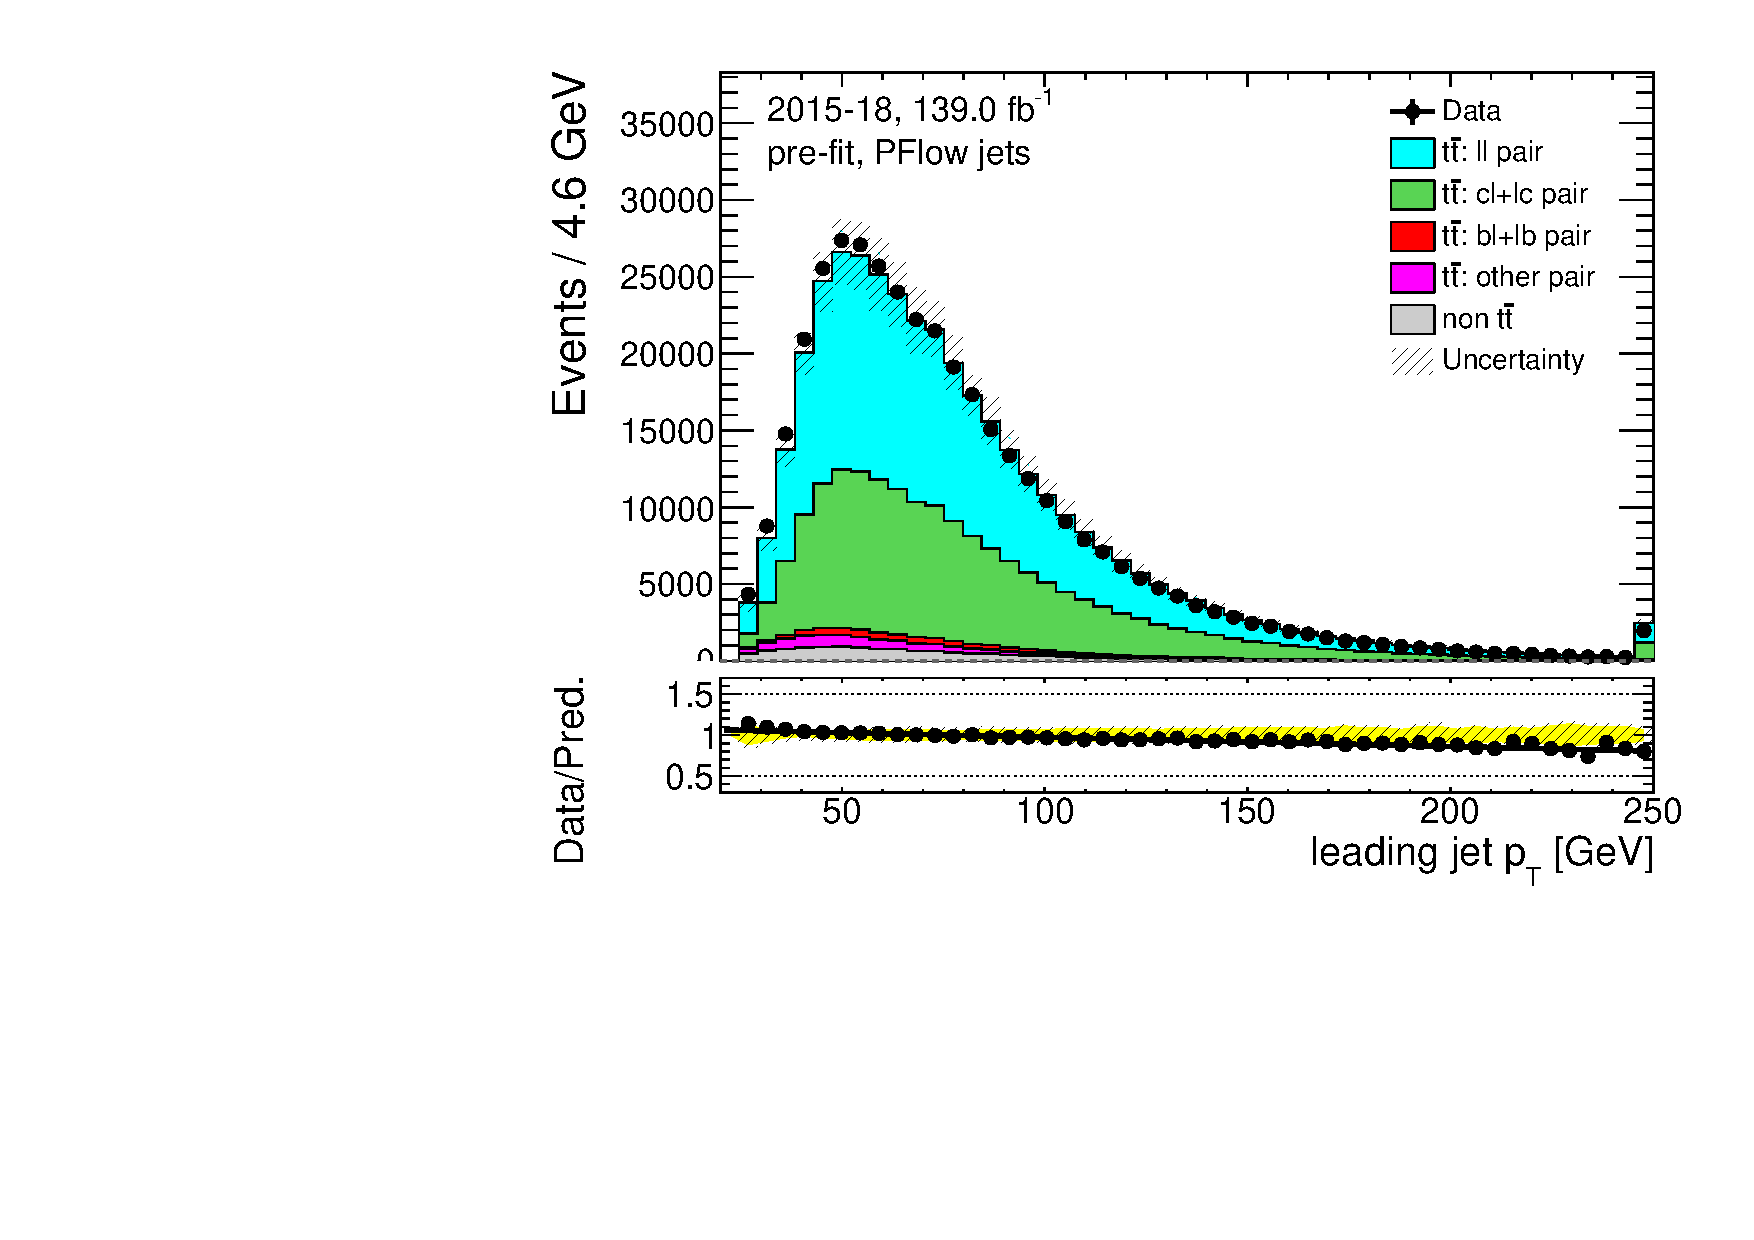
\includegraphics[width=0.45\textwidth]{FTAG_plots/pretagNoRwwithhighpTPFlowall/DataMC_h_J0_pt.pdf}
		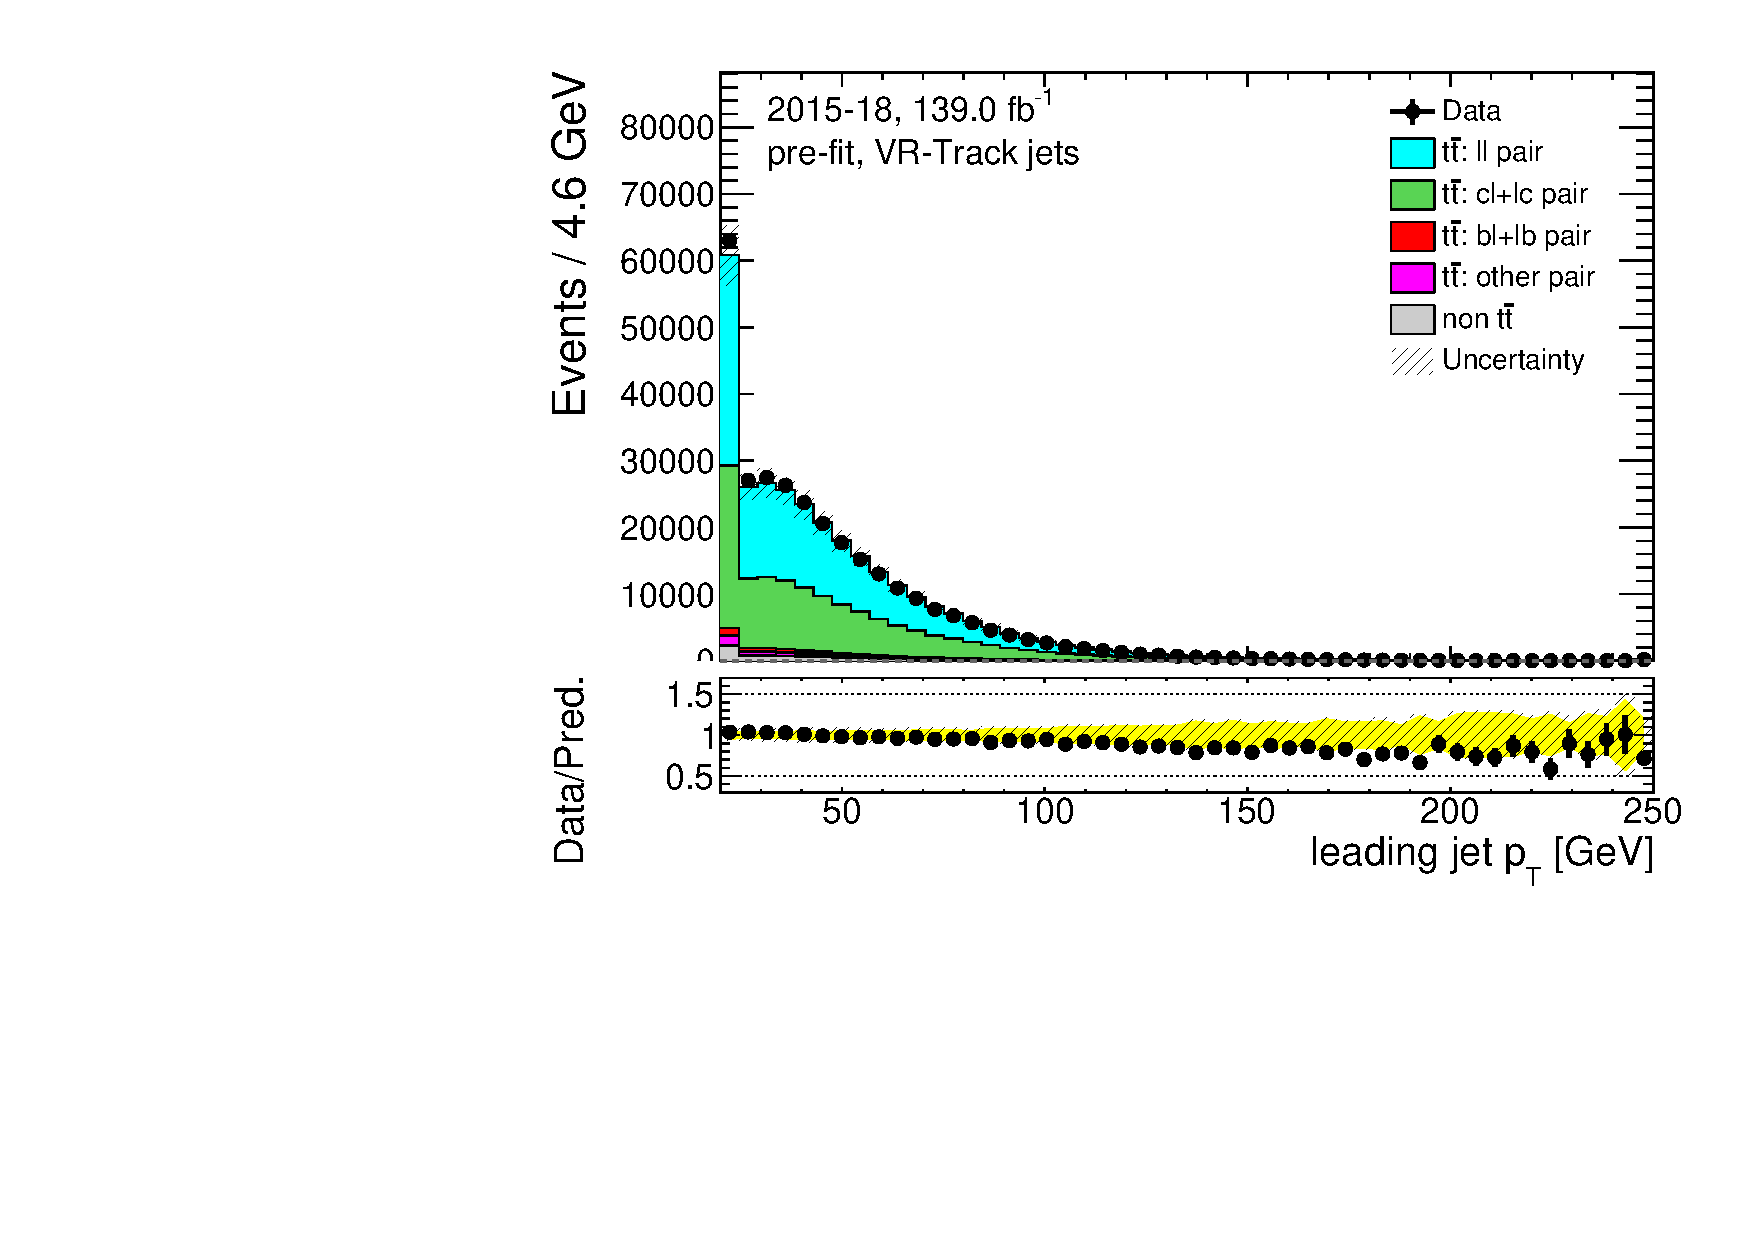
\includegraphics[width=0.45\textwidth]{FTAG_plots/pretagNoRwwithhighpTVRJetsall/DataMC_h_J0_pttrackjet.pdf}\\
		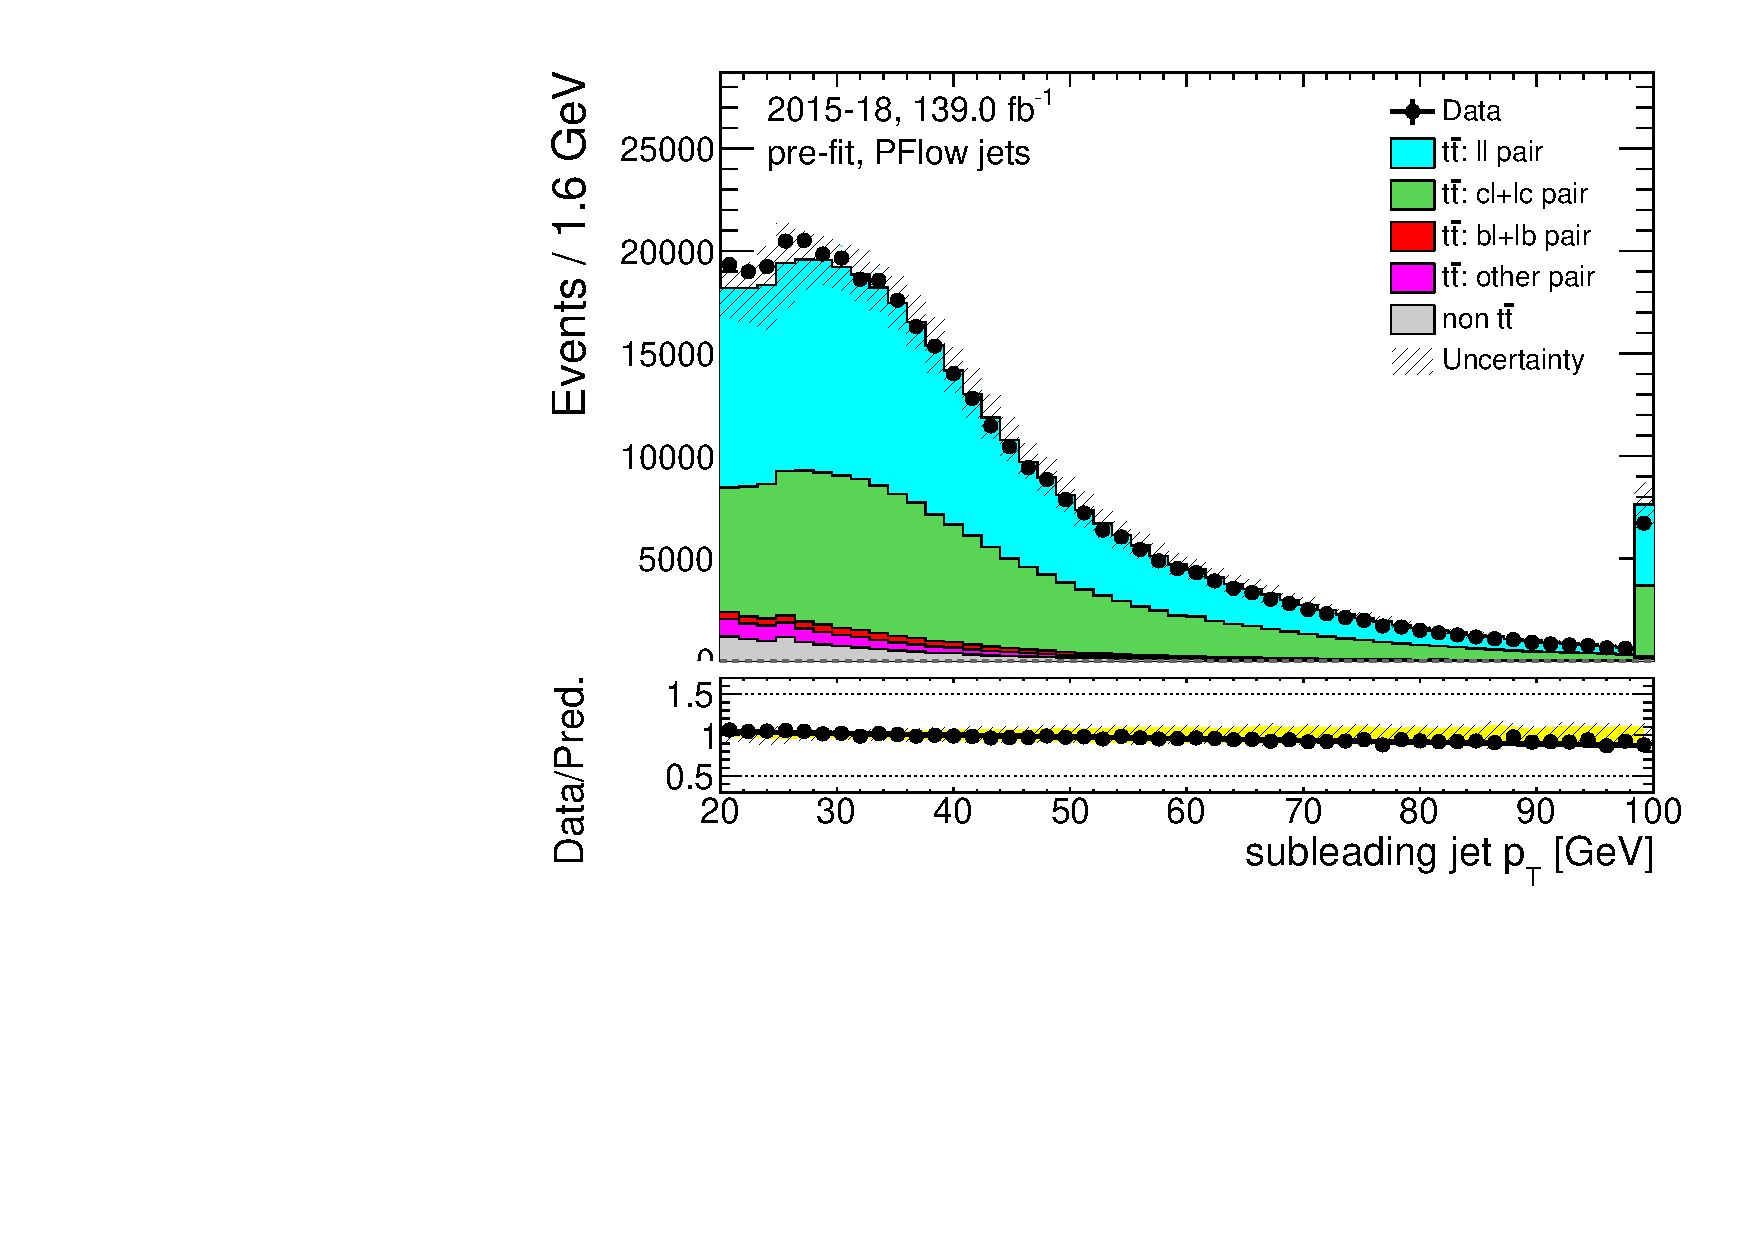
\includegraphics[width=0.45\textwidth]{FTAG_plots/pretagNoRwwithhighpTPFlowall/DataMC_h_J1_pt.pdf}
		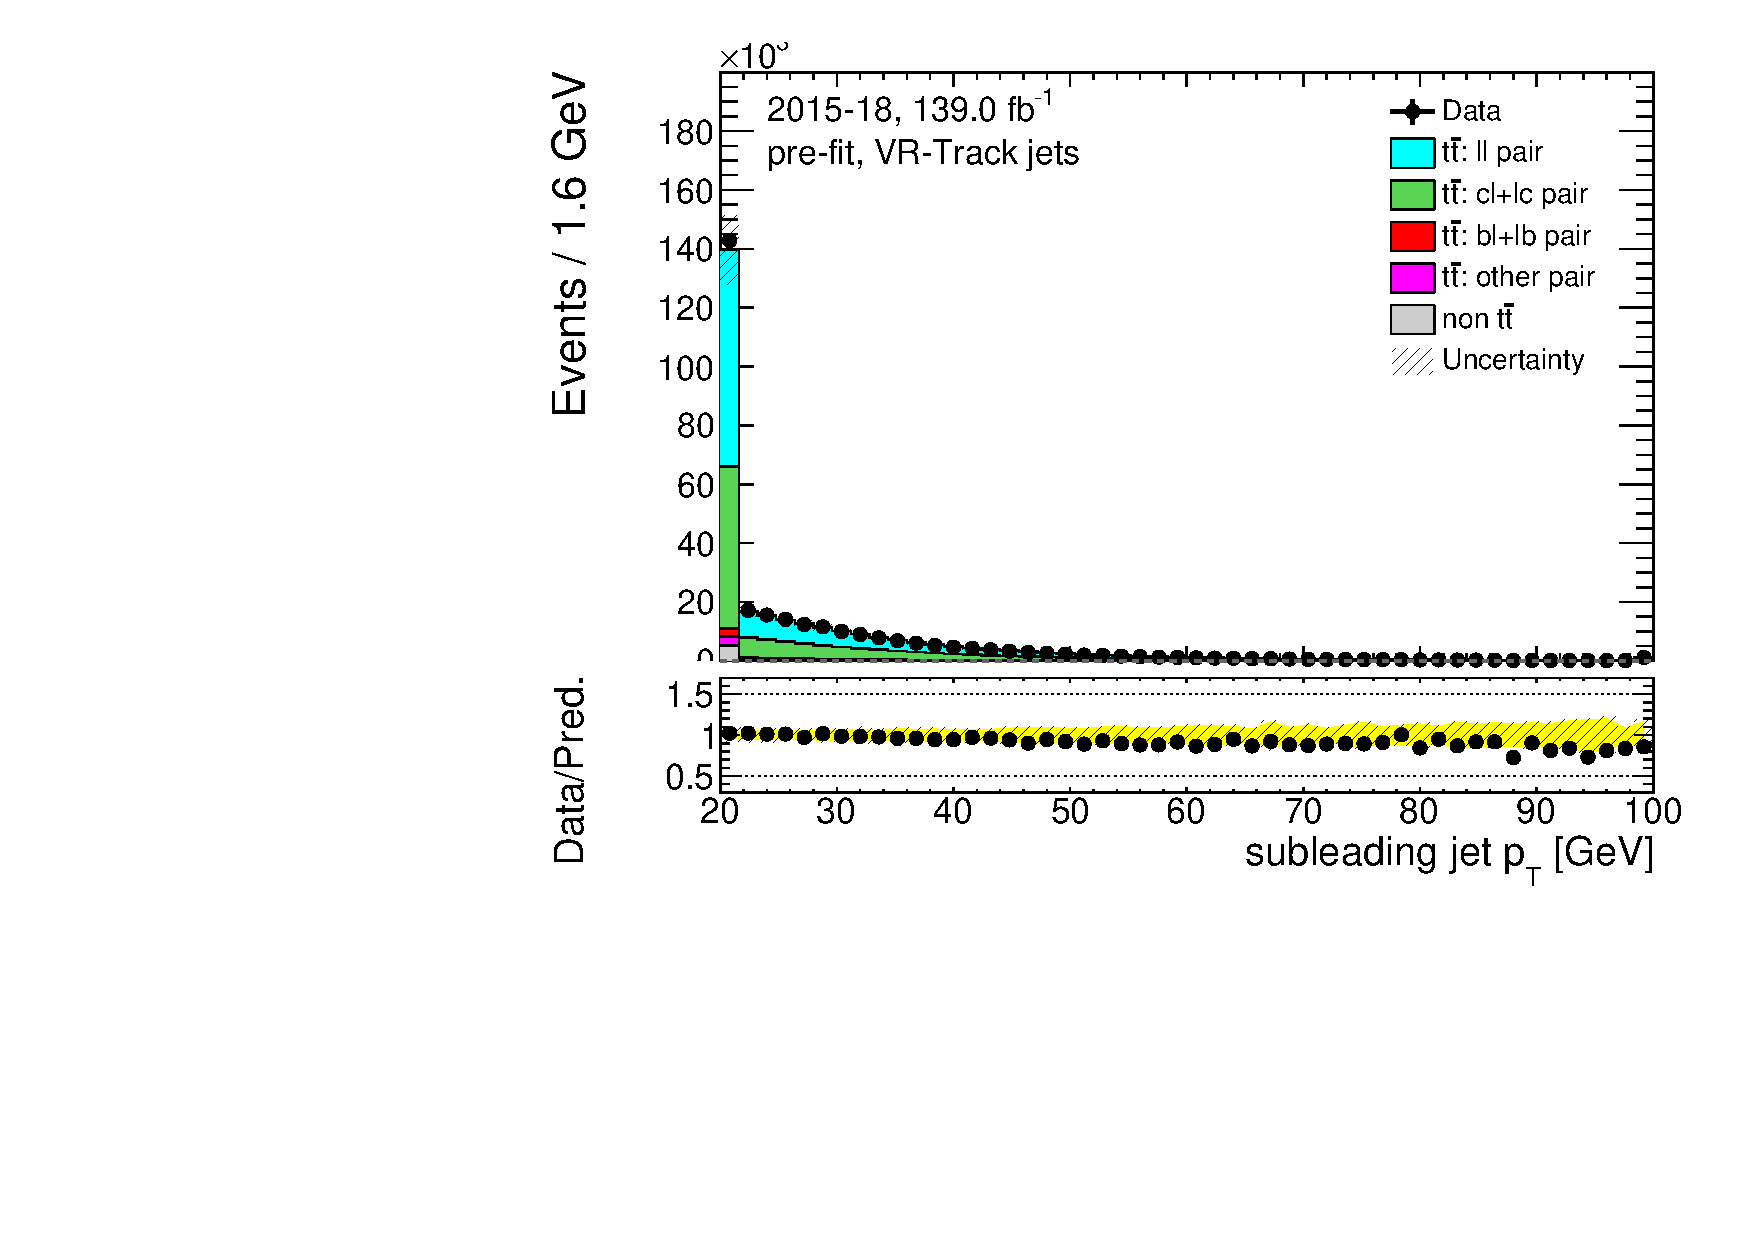
\includegraphics[width=0.45\textwidth]{FTAG_plots/pretagNoRwwithhighpTVRJetsall/DataMC_h_J1_pttrackjet.pdf}\\
		\caption{Combined selection: data versus simulation of $W$ jets\pt\ for 
		PFlow jets in the left column and for VR-Track jets in the right column.}
		\label{fig:kinematic_distributions_combined}
\end{figure}
		

\section{Systematic uncertainties}
\label{sec:FTAG_systematics}
The systematic uncertainties considered and propagated in this calibration 
can be broadly categorised into experimental and modelling systematic uncertainties. 
\subsection{Experimental uncertainties}
TODO: refer to the analysis Part
Experimental uncertainties are related to the detector and estimated using 
data-driven methods or MC simulations. 
The lepton energy scale and resolution are corrected to 
provide better agreement between MC predictions and data, uncertainties 
due the corrections are considered. Uncertainties are taken into account on the 
electron and muon trigger, identification and reconstruction efficiencies, and for 
uncertainties associated with the isolation requirements. 

The jet energy scale (JES) uncertainty depends on $p_T$ and $\eta$ and 
takes into account uncertainties due to pile-up effects. Uncertainties on the jet energy resolution (JER) 
are taken into account. Uncertainties on the energy scale and resolution of 
the electrons, muons, jets and taus are propagated to the calculation of the \MET, 
which also has additional dedicated uncertainties on the scale, resolution, and 
reconstruction efficiency of tracks not associated to any of the reconstructed objects,
 along with the modelling of the underlying event. Uncertainties on the $b$-tagging (mis-tagging) 
 probabilities for $b$ (light) jets are considered both for the tagging jets assigned to the $b$ quark 
 from the top decay and for the jets associated to the hadronically decaying $W$ boson.
Supporting material for this section can be found in the appendix, Tab.\ref{tab:systematics}.
%The uncertainty on these corrections is taken into account as a shape-dependent systematic uncertainty in the final fit of the backgrounds and signal models.

\subsection{Modelling uncertainties} 
The uncertaity due to different choices of the parton shower models is estimated by comparing
the MC samples generated with nominal parton shower model and with the 
alternative parton shower model.
More specifically, it is derived 
by comparing the prediction from \powheg interfaced either to \pythia or \Herwigpp. 
The uncertainty due to additional radiation in 
the initial state and the final state is estimated by comparing the nominal MC samples with the MC samples 
with alternative scale of renormalisation and factorisation.
The uncertainty on modelling of initial state radiation (ISR) is assessed with two alternative \powhegpythia 
samples. The samples include one with an increase in radiation which has the renormalisation and 
factorisation scales decreased by a factor of two and the \textit{hdamp} parameter doubled 
(which controls the \pt\ of the first additional emission), while 
the sample with a decrease in radiation has the scales increased by a factor of two. 
In all cases, MC-to-MC SFs are taken into account.
In addition, the uncertainty due to the
variations samples being produced by fast simulation while the nominal samples being 
produced full simulation is also considered.
The comparisons of 
the nominal \ttbar\ sample and the samples with each systematic uncertainty 
are shown in Table \ref{tab:modelling_syst}. 



\begin{table}[ht]
	\centering
	\small
	\setlength\tabcolsep{5pt} 
	\newcolumntype{C}{ @{}>{${}}c<{{}$}@{} }
	\begin{tabular}{|r *2{|rCr|r}| }
	\hline
	& \multicolumn{4}{|c|}{PFlow jets} & \multicolumn{4}{c|}{Track jets} \\
	\hline
	& \multicolumn{3}{c|}{Yields} & \specialcell{Ratio of \\difference to \\nominal sample} & \multicolumn{3}{c|}{Yields} & \specialcell{Ratio of \\difference to\\ nominal sample} \\
	\hline
	\ttbar\ Nominal &	 385378  &\pm&  230 &         &   	  302690 &\pm&  200   &  \\
	Data/MC         &        0.973  &\pm&  0.002 &      &     0.971 &\pm&  0.002 &         \\
	\hline
	\ttbar\ AF2     &    386260  &\pm&  250  &  0.716\% &     304860  &\pm&  230  &  0.716\%\\
	DATA/MC(AF2)    &    0.967  &\pm&  0.002  &          &    0.965  &\pm&  0.002   &      \\              
	\hline
	\ttbar\ ISR     &    377130  &\pm&  220  & -1.665\% &     297960  &\pm&  200  & -1.562\%\\     
	DATA/MC(ISR)    &    0.989  &\pm&  0.002  &          &    0.986  &\pm&  0.002   &  \\       
	\hline
	\ttbar\ \Herwig &    331960  &\pm&  220  & -13.443\%&     259940  &\pm&  190  & -14.123\%\\ 
	DATA/MC(\Herwig)&    1.119  &\pm&  0.002  &          &    1.126  &\pm&  0.002   &\\                
	\hline
	\end{tabular}
	\vspace{0.2cm}
	\caption{Comparison of the number of events in data and in 
	simulation considering the PFlow jets and the VR-Track jets for an inclusive
	selection. The uncertainty due to the variations samples being produced 
	by fast simulation is included in the table as \ttbar\ AF2. }
	\label{tab:modelling_syst}
	\end{table}


\section{Under-estimation of $t\bar{t}$ + Heavy flavour background }
Depsite the fact that the true nature of most of the reconstructed $W$ jets are either 
\cjets\ or light jets, there is still a very small amount of them are true \bjets. 

There are two main sources of these true \bjets. The first is a $W$ boson 
decays to a $b$ and a $c$ quark. The second is 
when the $t\bar{t}$ plus a gluon process (referred to as \ttbar\ + heavy flavour process)
is selected, and the gluon splits
into a pair a $b$ quarks and one of them is assigned as a $W$ jet. 
The first source can be excluded by requiring no \cjets in the $W$ jets,
meaning the true \bjet\ in the $W$ jets 
can only come from the $t\bar{t}$ + heavy flavour 
process. This process is underestimated by the MC by about 30\% 
for both the PFlow and VR-Track jets collections, as shown in Table \ref{tab:3byields1} 
and Figure~\ref{fig:3bplots}, where an extra cut requiring at least one $W$ jet with DL1r $> 8$ 
is added to the combined selection to reject most of the true \cjets and true light jet. 
A more thorough study is done in Ref.~\cite{TOPQ-2017-12}, where the mis-modelling 
factor is measured to be $1.25 \pm 0.25$, which is also consistent with the $30\%$ 
mismodelling observed in the previous study. 
Therefore, events in the simulation
in which the top jets and at least one of the $W$ jets are \bjets (referred to as 3 true \bjets\ events), 
are scaled by $1.25 \pm 0.25$.
All results shown in this chapter have this scale factor implemented, 
and the full difference between the simulation before applying this scale factor and 
after is taken as a systematic uncertainty. This uncertainty has been added in quadrature 
to the systematic uncertainties described in Section \ref{sec:FTAG_systematics} 
in all the plots in this chapter.



\begin{table}[ht]
    \centering
	\newcolumntype{C}{ @{}>{${}}c<{{}$}@{} }
	\begin{tabular}{|r *2{|rCr}| }
		\hline
		& \multicolumn{3}{|c|}{PFlow jets} & \multicolumn{3}{c|}{VR-Track jets} \\
		\hline
        Data & 1589& & & 1336  & & \\
         $t\bar{t}$ & 1100  &\pm&  13	& 940  &\pm&  12\\
         Non \ttbar\ 		& 83  &\pm&  6		& 69  &\pm&  5  \\
		 Data/MC 	& 1.34  &\pm&  0.04 & 1.32  &\pm&  0.04 \\
		 \hline
    \end{tabular}
	\caption{Yields of the 2018 data and MC of the combined selection, 
	requiring at least 1 PFlow or track $W$ jet with DL1r > 8 to 
	reject most of the light- and \cjets.}
    \label{tab:3byields1}
\end{table}


\begin{figure}[bth]
    \centering
\includegraphics[width=.45\textwidth]{FTAG_plots/3bplots/3bplots.png}
	\caption{The DL1r score distribution of the leading VR-Track jet, 
	requiring at least 1 VR-Track jets have DL1r > 8 to reject most of 
	the light and the $c$ jets, with $t\bar{t}$ modelling and statistical uncertainties. }
    \label{fig:3bplots}
\end{figure}


\section{Results}
\label{result}


\subsection{Overview}
Four rounds of calibrations have been carried out, containing different 
jet collections, Monte Carlo samples, analysis framework 
and \bjet\ identification algorithm. 
In the latest round, 
the calibration includes the PFlow jet and the VR-Track jet collection, 
and MV2c10, DL1 and DL1r taggers. The low-$p_T$ 
selection and the standard selection are carried out for all four 
calibrations, while the high-$p_T$ selection is only implemented 
in the latest calibration. 

\subsection{\btagging\ algorithms output distribution}
The distributions of the \btagging\ algorithm' output of 
the MC and the data of the latest calibration 
(December 2020) are shown in Figure~\ref{fig:taggers_PFlow} for the PFlow jets and 
Figure~\ref{fig:taggers_VRJets} for the VR-Track jets, 
combining the standard selection, low \pt\ and the high-$p_T$ selection. 
In these figure, the data events are compared against the simulation.
The majority of the events come from \ttbar\ production. There is only
a very small fraction of non \ttbar\ events. The $W$ jets pairs are mostly light jets 
pairs and \cjet\ light jet pairs, and a very small fraction of the pairs are 
\bjet\ light jet pairs or pairs containing one or more $\tau$ hadron(s). 
The yellow band in the lower pad indicates the overall systematic uncertainties
and the black band represents the \ttbar\ modelling systematic uncertainty, 
which dominates at low \btagging\ discriminant (DL1 or DL1r < 4). 
The experimental systematic uncertainty is in general very small. 
At high \btagging\ discriminant (DL1 or DL1r > 4), the
uncertainty due to the $1.25 \pm 0.25$ scale factor 
becomes more important. 
\begin{figure}[H]
	\begin{subfigure}[t]{1\linewidth}
	\includegraphics[width=.45\textwidth]{FTAG_plots/pretagNoRwwithhighpTPFlowall/DataMC_h_J0_DL1_log.png}
	\includegraphics[width=.45\textwidth]{FTAG_plots/pretagNoRwwithhighpTPFlowall/DataMC_h_J1_DL1_log.png}\\
	\caption{DL1 tagger output}
	\end{subfigure}
	\begin{subfigure}[t]{1\linewidth}
		\includegraphics[width=.45\textwidth]{FTAG_plots/pretagNoRwwithhighpTPFlowall/DataMC_h_J0_DL1r_log.png}
		\includegraphics[width=.45\textwidth]{FTAG_plots/pretagNoRwwithhighpTPFlowall/DataMC_h_J1_DL1r_log.png}\\
		\caption{DL1r tagger output}
	\end{subfigure}
	\begin{subfigure}[t]{1\linewidth}
	\includegraphics[width=.45\textwidth]{FTAG_plots/pretagNoRwwithhighpTPFlowall/DataMC_h_J0_MV2c10_log.png}
	\includegraphics[width=.45\textwidth]{FTAG_plots/pretagNoRwwithhighpTPFlowall/DataMC_h_J1_MV2c10_log.png}\\
	\caption{MV2c10 tagger output}
	\end{subfigure}
	\caption{PFlow jets: distributions of the DL1, DL1r and MV2c10 
	tagger outputs of the combined selection, 
	leading jet in the left column and sub-leading jet in the right column,
	before fitting or tagging with full uncertainties.} \label{fig:taggers_PFlow}
\end{figure}
\newpage
\begin{figure}[H]
	\begin{subfigure}[t]{1\linewidth}
	\includegraphics[width=.45\textwidth]{FTAG_plots/pretagNoRwwithhighpTVRJetsall/DataMC_h_J0_DL1trackjet_log.png}
	\includegraphics[width=.45\textwidth]{FTAG_plots/pretagNoRwwithhighpTVRJetsall/DataMC_h_J1_DL1trackjet_log.png}\\
	\caption{DL1 tagger output}
	\end{subfigure}
	\begin{subfigure}[t]{1\linewidth}
	\includegraphics[width=.45\textwidth]{FTAG_plots/pretagNoRwwithhighpTVRJetsall/DataMC_h_J0_DL1rtrackjet_log.png}
	\includegraphics[width=.45\textwidth]{FTAG_plots/pretagNoRwwithhighpTVRJetsall/DataMC_h_J1_DL1rtrackjet_log.png}\\
	\caption{DL1r tagger output}
	\end{subfigure}
	\begin{subfigure}[t]{1\linewidth}
	\includegraphics[width=.45\textwidth]{FTAG_plots/pretagNoRwwithhighpTVRJetsall/DataMC_h_J0_MV2c10_Fulltrackjet_log.png}
	\includegraphics[width=.45\textwidth]{FTAG_plots/pretagNoRwwithhighpTVRJetsall/DataMC_h_J1_MV2c10_Fulltrackjet_log.png}\\
	\caption{MV2c10 tagger output}
	\end{subfigure}
	\caption{VR-Track jets: distributions of the DL1, DL1r and MV2c10 tagger outputs of 
	the combined selection, 
	leading jet in the left column and sub-leading jet in the right column,
	before fitting or tagging with full uncertainties.} \label{fig:taggers_VRJets}
\end{figure}	

\subsection{Efficiencies and Scale Factors}
%The Monte Carlo simulation demonstrates good agreement in different kinematic variables with data. 
The Dl1 and DL1r \cjet efficiencies and scale factors with systematics 
uncertainties are calculated with four fixed cut working points 
for the PFlow and VR VR-Track jets collection in the latest derivation 
in December 2020.

The \cjet\ mis-tagging efficiencies are shown in Figure~\ref{fig:Dec_eff_PFlow_DL1}-\ref{fig:Dec_eff_VRJets_DL1r} 
for the PFlow jet collections and the VR-Track jets with the DL1 and the DL1r tagger. 
For PFlow jets, these results combine the standard selection, low\pt\ selection and the high-$p_T$ selection 
and for the VR-Track jets they combine the standard selection and the high-$p_T$ selection. 

The $1.25 \pm 0.25$ scale factor is applied on events with 3 true \bjets. 
The overall uncertainties are shown 
in the red band. 
The scale factors are shown in Figure~\ref{fig:Dec_SF_PFlow_DL1}-\ref{fig:Dec_SF_VRJets_DL1r} for the PFlow jets
and the VR-Track jets with the DL1 and DL1r tagger. 
The tighter working points (60\%, 70\%) show larger uncertainties and bigger deviation from 1, while
the looser working points (77\%, 85\%) have much smaller uncertainty and the simulation is able to 
recover the data well due to more abundant events statistics.
For the PFlow jets, in most of the working points the systematic uncertainties dominate 
in the low-\pt\ bins (\pt\ < 150) and the statistical error, represented by the error bars on the 
markers, become more important in the last bin. 
For the VR-Track jets the statistical uncertainty is relatively constant for all bins while the 
systematic uncertainty increases as the \pt\ increases. 
To demonstrate the effect on statistics with the high-\pt\ selection, 
the fractional statistical uncertainties of 60\% working point scale factor
are shown in Table \ref{tab:stats_gain} for the standard and the combined selection.
In some bins the statistical uncertainty can decrease up to 30\%, suggesting that the
high-\pt\ selection is successful at increasing events statistics. 

\begin{table}[ht]
	\centering
	\small
	\setlength\tabcolsep{5pt} 
	\begin{tabular}{|r *2{|rr|r}| }
	\hline
	& \multicolumn{3}{|c|}{PFlow jets} & \multicolumn{3}{c|}{VR-Track jets} \\
	\hline
	&  \specialcell{Standard\\ selection} &\specialcell{ High-\pt\ \\selection }&\specialcell{ Fractional \\decrease} &  \specialcell{Standard\\ selection} &\specialcell{ High-\pt\ \\selection }&\specialcell{ Fractional \\decrease}\\
	\hline
	Bin No.1    &	 3.3\%  &3.3\% & 0.0\% & 5.6\%  & 5.3\%      &  5.7\%  \\
	Bin No.2    &    3.1\%  &2.8\% & 10.7\% & 4.2\%  & 3.7\%     & 13.5\%   \\
	Bin No.3    &    3.4\%  &2.6\% & 30.8\% & 5.8\%  & 4.9\%     & 18.4\%   \\
	Bin No.4    &    12.1\% &9.3\% & 30.1\% & 7.2\%  & 5.6\%     & 28.6\%   \\           
	\hline                 
	\end{tabular}
	\vspace{0.2cm}
	\caption{Comparison of the fractional statistical uncertainty in the DL1r 60\%
	working point scale factor. The \pt\ range of each bin can be found in section \ref{sec:Calibration method for charm jet}. }
	\label{tab:stats_gain}
	\end{table}



\newpage
%%% Efficiencies plots %%%

\begin{figure}[H]
	\centering
	\begin{subfigure}[t]{.35\linewidth}
\includegraphics[width=1\textwidth]{FTAG_plots/DL1allPFlowDec/eff60.eps}
\caption{60\% working point}
	\end{subfigure}
\begin{subfigure}[t]{.35\linewidth}
	\includegraphics[width=1\textwidth]{FTAG_plots/DL1allPFlowDec/eff70.eps}
	\caption{70\% working point}
\end{subfigure}
\begin{subfigure}[t]{.35\linewidth}
\includegraphics[width=1\textwidth]{FTAG_plots/DL1allPFlowDec/eff77.eps}
\caption{77\% working point}
\end{subfigure}
\begin{subfigure}[t]{.35\linewidth}
\includegraphics[width=1\textwidth]{FTAG_plots/DL1allPFlowDec/eff85.eps}
\caption{85\% working point}
\end{subfigure}
\caption{Charm-jet efficiencies for the PFlow jets collection with
the DL1 tagger.} \label{fig:Dec_eff_PFlow_DL1}
\end{figure}

\begin{figure}[H]
	\centering
	\begin{subfigure}[t]{.35\linewidth}
		\includegraphics[width=1\textwidth]{FTAG_plots/DL1rallPFlowDec/eff60.eps}
		\caption{60\% working point}
			\end{subfigure}
		\begin{subfigure}[t]{.35\linewidth}
			\includegraphics[width=1\textwidth]{FTAG_plots/DL1rallPFlowDec/eff70.eps}
			\caption{70\% working point}
		\end{subfigure}
		\begin{subfigure}[t]{.35\linewidth}
		\includegraphics[width=1\textwidth]{FTAG_plots/DL1rallPFlowDec/eff77.eps}
		\caption{77\% working point}
		\end{subfigure}
		\begin{subfigure}[t]{.35\linewidth}
		\includegraphics[width=1\textwidth]{FTAG_plots/DL1rallPFlowDec/eff85.eps}
		\caption{85\% working point}
		\end{subfigure}
		\caption{Charm-jet efficiencies for the PFlow jets collection with
	the DL1r tagger.} \label{fig:Dec_eff_PFlow_DL1r}
\end{figure}


\newpage
\begin{figure}[H]
	\centering
	\begin{subfigure}[t]{.35\linewidth}
		\includegraphics[width=1\textwidth]{FTAG_plots/DL1allVRJetsDec/eff60.eps}
		\caption{60\% working point}
			\end{subfigure}
		\begin{subfigure}[t]{.35\linewidth}
			\includegraphics[width=1\textwidth]{FTAG_plots/DL1allVRJetsDec/eff70.eps}
			\caption{70\% working point}
		\end{subfigure}
		\begin{subfigure}[t]{.35\linewidth}
		\includegraphics[width=1\textwidth]{FTAG_plots/DL1allVRJetsDec/eff77.eps}
		\caption{77\% working point}
		\end{subfigure}
		\begin{subfigure}[t]{.35\linewidth}
		\includegraphics[width=1\textwidth]{FTAG_plots/DL1allVRJetsDec/eff85.eps}
		\caption{85\% working point}
		\end{subfigure}
	\caption{Charm-jet efficiencies for the VR-Track jets collection with
	the DL1 tagger.} \label{fig:Dec_eff_VRJets_DL1}
	\end{figure}

	\begin{figure}[H]
		\centering
		\begin{subfigure}[t]{.35\linewidth}
			\includegraphics[width=1\textwidth]{FTAG_plots/DL1rallVRJetsDec/eff60.eps}
			\caption{60\% working point}
				\end{subfigure}
			\begin{subfigure}[t]{.35\linewidth}
				\includegraphics[width=1\textwidth]{FTAG_plots/DL1rallVRJetsDec/eff70.eps}
				\caption{70\% working point}
			\end{subfigure}
			\begin{subfigure}[t]{.35\linewidth}
			\includegraphics[width=1\textwidth]{FTAG_plots/DL1rallVRJetsDec/eff77.eps}
			\caption{77\% working point}
			\end{subfigure}
			\begin{subfigure}[t]{.35\linewidth}
			\includegraphics[width=1\textwidth]{FTAG_plots/DL1rallVRJetsDec/eff85.eps}
			\caption{85\% working point}
			\end{subfigure}
		\caption{Charm-jet efficiencies for the VR-Track jets collection with
		the DL1r tagger.} \label{fig:Dec_eff_VRJets_DL1r}
\end{figure}

\newpage
%SF plots
\begin{figure}[H]
	\centering
	\begin{subfigure}[t]{.35\linewidth}
		\includegraphics[width=1\textwidth]{FTAG_plots/DL1allPFlowDec/SF60.eps}
		\caption{60\% working point}
			\end{subfigure}
		\begin{subfigure}[t]{.35\linewidth}
			\includegraphics[width=1\textwidth]{FTAG_plots/DL1allPFlowDec/SF70.eps}
			\caption{70\% working point}
		\end{subfigure}
		\begin{subfigure}[t]{.35\linewidth}
		\includegraphics[width=1\textwidth]{FTAG_plots/DL1allPFlowDec/SF77.eps}
		\caption{77\% working point}
		\end{subfigure}
		\begin{subfigure}[t]{.35\linewidth}
		\includegraphics[width=1\textwidth]{FTAG_plots/DL1allPFlowDec/SF85.eps}
		\caption{85\% working point}
		\end{subfigure}
	\caption{Charm-jet scale factors for the PFlow jets collection with 
	the DL1 tagger.} \label{fig:Dec_SF_PFlow_DL1}
	\end{figure}
	

\begin{figure}[H]
	\centering
	\begin{subfigure}[t]{.35\linewidth}
		\includegraphics[width=1\textwidth]{FTAG_plots/DL1rallPFlowDec/SF60.eps}
		\caption{60\% working point}
			\end{subfigure}
		\begin{subfigure}[t]{.35\linewidth}
			\includegraphics[width=1\textwidth]{FTAG_plots/DL1rallPFlowDec/SF70.eps}
			\caption{70\% working point}
		\end{subfigure}
		\begin{subfigure}[t]{.35\linewidth}
		\includegraphics[width=1\textwidth]{FTAG_plots/DL1rallPFlowDec/SF77.eps}
		\caption{77\% working point}
		\end{subfigure}
		\begin{subfigure}[t]{.35\linewidth}
		\includegraphics[width=1\textwidth]{FTAG_plots/DL1rallPFlowDec/SF85.eps}
		\caption{85\% working point}
		\end{subfigure}
	\caption{Charm-jet scale factors for the PFlow jets collection with 
	the DL1r tagger.} \label{fig:Dec_SF_PFlow_DL1r}
	\end{figure}	
\newpage
\begin{figure}[H]
	\centering
	\begin{subfigure}[t]{.35\linewidth}
		\includegraphics[width=1\textwidth]{FTAG_plots/DL1allVRJetsDec/SF60.eps}
		\caption{60\% working point}
			\end{subfigure}
		\begin{subfigure}[t]{.35\linewidth}
			\includegraphics[width=1\textwidth]{FTAG_plots/DL1allVRJetsDec/SF70.eps}
			\caption{70\% working point}
		\end{subfigure}
		\begin{subfigure}[t]{.35\linewidth}
		\includegraphics[width=1\textwidth]{FTAG_plots/DL1allVRJetsDec/SF77.eps}
		\caption{77\% working point}
		\end{subfigure}
		\begin{subfigure}[t]{.35\linewidth}
		\includegraphics[width=1\textwidth]{FTAG_plots/DL1allVRJetsDec/SF85.eps}
		\caption{85\% working point}
		\end{subfigure}
	\caption{Charm-jet scale factors for the VR-Track jets collection with 
	the DL1 tagger.} \label{fig:Dec_SF_VRJets_DL1}
	\end{figure}
	

\begin{figure}[H]
	\centering
	\begin{subfigure}[t]{.35\linewidth}
		\includegraphics[width=1\textwidth]{FTAG_plots/DL1rallVRJetsDec/SF60.eps}
		\caption{60\% working point}
			\end{subfigure}
		\begin{subfigure}[t]{.35\linewidth}
			\includegraphics[width=1\textwidth]{FTAG_plots/DL1rallVRJetsDec/SF70.eps}
			\caption{70\% working point}
		\end{subfigure}
		\begin{subfigure}[t]{.35\linewidth}
		\includegraphics[width=1\textwidth]{FTAG_plots/DL1rallVRJetsDec/SF77.eps}
		\caption{77\% working point}
		\end{subfigure}
		\begin{subfigure}[t]{.35\linewidth}
		\includegraphics[width=1\textwidth]{FTAG_plots/DL1rallVRJetsDec/SF85.eps}
		\caption{85\% working point}
		\end{subfigure}
	\caption{Charm-jet scale factors for the VR-Track jets collection with 
	the DL1r tagger.} \label{fig:Dec_SF_VRJets_DL1r}
	\end{figure}	


\newpage
\iffalse


In terms of statistical gain, taking the 60\% working point scale factor with 2018 data as an example, the error is reduced as expected. In the last bin of the $p_{T}$ distribution of scale factors, the error is reduced by 55\%, which suggests the success of high-$p_{T}$ selection method. The percentage reduction of error of each bin is given in Tab.\ref{tab:limit}:


 \begin{table}[ht]
 \begin{centering}
 \begin{tabular}{|p{2.5em}||p{2.5em}|p{2.5em}|p{5em}||p{2.5em}|p{2.5em}|p{5em}||p{5em}|}
          \hline
          & \multicolumn{3}{|c||}{high-$p_{T}$ + standard selection} & \multicolumn{3}{|c||}{standard selection only} & \\  \hline\hline
          Bins& Bin Value &Bin error&Percentage error&Bin Value &Bin error&Percentage error & Error reduction\\ \hline
          Bin 1 & 1.25 & 0.12 & 10\% &1.20 & 0.13 & 11\% & 11\% \\ \hline
          Bin 2 & 1.34 & 0.10 & 8\% & 1.24 & 0.11 & 9\% & 18\% \\ \hline
          Bin 3 & 1.22 & 0.10 & 8\% & 1.04 & 0.11 & 10\% & 28\% \\ \hline
          Bin 4 & 0.98 & 0.24 & 24\% & 0.72 & 0.27 & 37\% & 55\% \\ \hline
          
 
 \end{tabular} 
 \caption{Bins values and the corresponding errors of the scale factor at 60\% working point, with 2018 data.}
 \end{centering}
 \label{tab:limit}
 \end{table}

\fi

\newpage




\large
\chapter{Search for Higgs boson pair production in the \bbtt\ channel}
\label{sec:search for dihiggs}
\section{Data and Monte Carlo samples}
\section{Trigger and event selection}
\label{sec:event selection}
\section{Background estimation}
\section{Multivariate analysis}
\section{Systematic uncertainties}
\section{Results}
\chapter{Summary}

\printbibliography
\appendix

\chapter{Supplementary material for \texorpdfstring{\cjet}{c-jet} calibration}
\section{Additional plots for kinematic variables}
\subsection{Standard selection}

\label{sec:appendix_standard_selection}
\newpage	
\begin{figure}[H]
\includegraphics[width=.45\textwidth]{FTAG_plots/pretagNoRwwithouthighpTPFlowall/DataMC_h_J0_eta.png}
\includegraphics[width=.45\textwidth]{FTAG_plots/pretagNoRwwithouthighpTPFlowall/DataMC_h_J1_eta.png}\\
\includegraphics[width=.45\textwidth]{FTAG_plots/pretagNoRwwithouthighpTPFlowall/DataMC_h_LLR.png}
\includegraphics[width=.45\textwidth]{FTAG_plots/pretagNoRwwithouthighpTPFlowall/DataMC_h_MET.png}\\

\caption{PFlow jets: distributions of the leading and sub-leading jets 
from W decay, KLFitter output and the transverse missing transverse 
energy of the standard selection, before fitting or tagging with 
full uncertainties.} \label{fig:standard_jets_PFlow}
\end{figure}

\newpage
\begin{figure}[H]
\includegraphics[width=.45\textwidth]{FTAG_plots/pretagNoRwwithouthighpTPFlowall/DataMC_h_dRbb.png}
\includegraphics[width=.45\textwidth]{FTAG_plots/pretagNoRwwithouthighpTPFlowall/DataMC_h_dRqq.png}\\
\includegraphics[width=.45\textwidth]{FTAG_plots/pretagNoRwwithouthighpTPFlowall/DataMC_h_dRbhadq1.png}
\includegraphics[width=.45\textwidth]{FTAG_plots/pretagNoRwwithouthighpTPFlowall/DataMC_h_dRblepq1.png} \\
\includegraphics[width=.45\textwidth]{FTAG_plots/pretagNoRwwithouthighpTPFlowall/DataMC_h_dRWhadbhad.png} 
\includegraphics[width=.45\textwidth]{FTAG_plots/pretagNoRwwithouthighpTPFlowall/DataMC_h_dRWhadblep.png} \\
\caption{PFlow jets: distributions of angle related variables of the combination of the standard selection,
 before fitting or 
tagging with full uncertainties.} \label{fig:standard_angles_PFlow}
\end{figure}

\newpage
\begin{figure}[H]
\includegraphics[width=.45\textwidth]{FTAG_plots/pretagNoRwwithouthighpTPFlowall/DataMC_h_Mbb.png}
\includegraphics[width=.45\textwidth]{FTAG_plots/pretagNoRwwithouthighpTPFlowall/DataMC_h_mjj.png}\\
\includegraphics[width=.45\textwidth]{FTAG_plots/pretagNoRwwithouthighpTPFlowall/DataMC_h_mjjj.png}
\includegraphics[width=.45\textwidth]{FTAG_plots/pretagNoRwwithouthighpTPFlowall/DataMC_h_Htjj.png}\\
\caption{PFlow jets: distributions of mass related variables of the standard selection, 
before fitting or 
tagging with stat-only uncertainties.} \label{fig:standard_mass_PFlow}
\end{figure}



\newpage	
\begin{figure}[H]
\includegraphics[width=.45\textwidth]{FTAG_plots/pretagNoRwwithouthighpTVRJetsall/DataMC_h_J0_etatrackjet.png}
\includegraphics[width=.45\textwidth]{FTAG_plots/pretagNoRwwithouthighpTVRJetsall/DataMC_h_J1_etatrackjet.png}\\
\includegraphics[width=.45\textwidth]{FTAG_plots/pretagNoRwwithouthighpTVRJetsall/DataMC_h_LLRtrackjet.png}
\includegraphics[width=.45\textwidth]{FTAG_plots/pretagNoRwwithouthighpTVRJetsall/DataMC_h_METtrackjet.png}\\

\caption{VR-Track jets: distributions of the leading and sub-leading jets 
from W decay, KLFitter output and the transverse missing transverse 
energy of the standard selection, before fitting or tagging with 
full uncertainties.} \label{fig:standard_jets_VRJets}
\end{figure}



\newpage
\begin{figure}[H]
\includegraphics[width=.45\textwidth]{FTAG_plots/pretagNoRwwithouthighpTVRJetsall/DataMC_h_dRbbtrackjet.png}
\includegraphics[width=.45\textwidth]{FTAG_plots/pretagNoRwwithouthighpTVRJetsall/DataMC_h_dRqqtrackjet.png}\\
\includegraphics[width=.45\textwidth]{FTAG_plots/pretagNoRwwithouthighpTVRJetsall/DataMC_h_dRbhadq1trackjet.png}
\includegraphics[width=.45\textwidth]{FTAG_plots/pretagNoRwwithouthighpTVRJetsall/DataMC_h_dRblepq1trackjet.png} \\
\includegraphics[width=.45\textwidth]{FTAG_plots/pretagNoRwwithouthighpTVRJetsall/DataMC_h_dRWhadbhadtrackjet.png} 
\includegraphics[width=.45\textwidth]{FTAG_plots/pretagNoRwwithouthighpTVRJetsall/DataMC_h_dRWhadbleptrackjet.png} \\
\caption{VR-Track jets: distributions of angle related variables of the combination 
of the standard selection, before fitting or tagging with full uncertainties.} \label{fig:standard_angles_VRJets}
\end{figure}

\newpage
\begin{figure}[H]
\includegraphics[width=.45\textwidth]{FTAG_plots/pretagNoRwwithouthighpTVRJetsall/DataMC_h_Mbbtrackjet.png}
\includegraphics[width=.45\textwidth]{FTAG_plots/pretagNoRwwithouthighpTVRJetsall/DataMC_h_mjjtrackjet.png}\\
\includegraphics[width=.45\textwidth]{FTAG_plots/pretagNoRwwithouthighpTVRJetsall/DataMC_h_mjjjtrackjet.png}
\includegraphics[width=.45\textwidth]{FTAG_plots/pretagNoRwwithouthighpTVRJetsall/DataMC_h_Htjjtrackjet.png}\\
\caption{VR-Track jets: distributions of mass related variables of the standard selection, 
before fitting or tagging with stat-only uncertainties.} \label{fig:standard_mass_VRJets}
\end{figure}


\subsection{Low-\texorpdfstring{\pt}{pT} selection}
\label{sec:appendix_lowpT_selection}
\newpage	
\begin{figure}[H]
\includegraphics[width=.45\textwidth]{FTAG_plots/pretagNoRwLowpTPFlowall/DataMC_h_J0_eta.png}
\includegraphics[width=.45\textwidth]{FTAG_plots/pretagNoRwLowpTPFlowall/DataMC_h_J1_eta.png}\\
\includegraphics[width=.45\textwidth]{FTAG_plots/pretagNoRwLowpTPFlowall/DataMC_h_LLR.png}
\includegraphics[width=.45\textwidth]{FTAG_plots/pretagNoRwLowpTPFlowall/DataMC_h_MET.png}\\

\caption{PFlow jets: distributions of the leading and sub-leading jets 
from W decay, KLFitter output and the transverse missing transverse 
energy of the low-\pt\ selection, before fitting or tagging with 
full uncertainties.} \label{fig:lowpT_jets_VRJets}
\end{figure}

\newpage
\begin{figure}[H]
\includegraphics[width=.45\textwidth]{FTAG_plots/pretagNoRwLowpTPFlowall/DataMC_h_dRbb.png}
\includegraphics[width=.45\textwidth]{FTAG_plots/pretagNoRwLowpTPFlowall/DataMC_h_dRqq.png}\\
\includegraphics[width=.45\textwidth]{FTAG_plots/pretagNoRwLowpTPFlowall/DataMC_h_dRbhadq1.png}
\includegraphics[width=.45\textwidth]{FTAG_plots/pretagNoRwLowpTPFlowall/DataMC_h_dRblepq1.png} \\
\includegraphics[width=.45\textwidth]{FTAG_plots/pretagNoRwLowpTPFlowall/DataMC_h_dRWhadbhad.png} 
\includegraphics[width=.45\textwidth]{FTAG_plots/pretagNoRwLowpTPFlowall/DataMC_h_dRWhadblep.png} \\
\caption{PFlow jets: distributions of angle related variables of the combination of the low-\pt\ selection,
 before fitting or 
tagging with full uncertainties.} \label{fig:lowpT_angles_PFlow}
\end{figure}

\newpage
\begin{figure}[H]
\includegraphics[width=.45\textwidth]{FTAG_plots/pretagNoRwLowpTPFlowall/DataMC_h_Mbb.png}
\includegraphics[width=.45\textwidth]{FTAG_plots/pretagNoRwLowpTPFlowall/DataMC_h_mjj.png}\\
\includegraphics[width=.45\textwidth]{FTAG_plots/pretagNoRwLowpTPFlowall/DataMC_h_mjjj.png}
\includegraphics[width=.45\textwidth]{FTAG_plots/pretagNoRwLowpTPFlowall/DataMC_h_Htjj.png}\\
\caption{PFlow jets: distributions of mass related variables of the low-\pt\ selection, 
before fitting or 
tagging with stat-only uncertainties.} \label{fig:lowpT_mass_PFlow}
\end{figure}

\section{High-\texorpdfstring{\pt}{pT} selection}
\label{sec:appendix_highpT_selection}
\newpage	
\begin{figure}[H]
\includegraphics[width=.45\textwidth]{FTAG_plots/pretagNoRwnewonlyPFlowall/DataMC_h_J0_eta.png}
\includegraphics[width=.45\textwidth]{FTAG_plots/pretagNoRwnewonlyPFlowall/DataMC_h_J1_eta.png}\\
\includegraphics[width=.45\textwidth]{FTAG_plots/pretagNoRwnewonlyPFlowall/DataMC_h_LLR.png}
\includegraphics[width=.45\textwidth]{FTAG_plots/pretagNoRwnewonlyPFlowall/DataMC_h_MET.png}\\

\caption{PFlow jets: distributions of the leading and sub-leading jets 
from W decay, KLFitter output and the transverse missing transverse 
energy of the high-\pt\ selection, before fitting or tagging with 
full uncertainties.} \label{fig:highpT_jets_PFlow}
\end{figure}

\newpage
\begin{figure}[H]
\includegraphics[width=.45\textwidth]{FTAG_plots/pretagNoRwnewonlyPFlowall/DataMC_h_dRbb.png}
\includegraphics[width=.45\textwidth]{FTAG_plots/pretagNoRwnewonlyPFlowall/DataMC_h_dRqq.png}\\
\includegraphics[width=.45\textwidth]{FTAG_plots/pretagNoRwnewonlyPFlowall/DataMC_h_dRbhadq1.png}
\includegraphics[width=.45\textwidth]{FTAG_plots/pretagNoRwnewonlyPFlowall/DataMC_h_dRblepq1.png} \\
\includegraphics[width=.45\textwidth]{FTAG_plots/pretagNoRwnewonlyPFlowall/DataMC_h_dRWhadbhad.png} 
\includegraphics[width=.45\textwidth]{FTAG_plots/pretagNoRwnewonlyPFlowall/DataMC_h_dRWhadblep.png} \\
\caption{PFlow jets: distributions of angle related variables of the combination of the high-\pt\ selection,
 before fitting or 
tagging with full uncertainties.} \label{fig:highpT_angles_PFlow}
\end{figure}

\newpage
\begin{figure}[H]
\includegraphics[width=.45\textwidth]{FTAG_plots/pretagNoRwnewonlyPFlowall/DataMC_h_Mbb.png}
\includegraphics[width=.45\textwidth]{FTAG_plots/pretagNoRwnewonlyPFlowall/DataMC_h_mjj.png}\\
\includegraphics[width=.45\textwidth]{FTAG_plots/pretagNoRwnewonlyPFlowall/DataMC_h_mjjj.png}
\includegraphics[width=.45\textwidth]{FTAG_plots/pretagNoRwnewonlyPFlowall/DataMC_h_Htjj.png}\\
\caption{PFlow jets: distributions of mass related variables of the high-\pt\ selection, 
before fitting or 
tagging with stat-only uncertainties.} \label{fig:highpT_mass_PFlow}
\end{figure}



\newpage	
\begin{figure}[H]
\includegraphics[width=.45\textwidth]{FTAG_plots/pretagNoRwnewonlyVRJetsall/DataMC_h_J0_etatrackjet.png}
\includegraphics[width=.45\textwidth]{FTAG_plots/pretagNoRwnewonlyVRJetsall/DataMC_h_J1_etatrackjet.png}\\
\includegraphics[width=.45\textwidth]{FTAG_plots/pretagNoRwnewonlyVRJetsall/DataMC_h_LLRtrackjet.png}
\includegraphics[width=.45\textwidth]{FTAG_plots/pretagNoRwnewonlyVRJetsall/DataMC_h_METtrackjet.png}\\

\caption{VR-Track jets: distributions of the leading and sub-leading jets 
from W decay, KLFitter output and the transverse missing transverse 
energy of the high-\pt\ selection, before fitting or tagging with 
full uncertainties.} \label{fig:highpT_jets_VRJets}
\end{figure}



\newpage
\begin{figure}[H]
\includegraphics[width=.45\textwidth]{FTAG_plots/pretagNoRwnewonlyVRJetsall/DataMC_h_dRbbtrackjet.png}
\includegraphics[width=.45\textwidth]{FTAG_plots/pretagNoRwnewonlyVRJetsall/DataMC_h_dRqqtrackjet.png}\\
\includegraphics[width=.45\textwidth]{FTAG_plots/pretagNoRwnewonlyVRJetsall/DataMC_h_dRbhadq1trackjet.png}
\includegraphics[width=.45\textwidth]{FTAG_plots/pretagNoRwnewonlyVRJetsall/DataMC_h_dRblepq1trackjet.png} \\
\includegraphics[width=.45\textwidth]{FTAG_plots/pretagNoRwnewonlyVRJetsall/DataMC_h_dRWhadbhadtrackjet.png} 
\includegraphics[width=.45\textwidth]{FTAG_plots/pretagNoRwnewonlyVRJetsall/DataMC_h_dRWhadbleptrackjet.png} \\
\caption{VR-Track jets: distributions of angle related variables of the combination 
of the high-\pt\ selection, before fitting or tagging with full uncertainties.} \label{fig:highpT_angles_VRJets}
\end{figure}

\newpage
\begin{figure}[H]
\includegraphics[width=.45\textwidth]{FTAG_plots/pretagNoRwnewonlyVRJetsall/DataMC_h_Mbbtrackjet.png}
\includegraphics[width=.45\textwidth]{FTAG_plots/pretagNoRwnewonlyVRJetsall/DataMC_h_mjjtrackjet.png}\\
\includegraphics[width=.45\textwidth]{FTAG_plots/pretagNoRwnewonlyVRJetsall/DataMC_h_mjjjtrackjet.png}
\includegraphics[width=.45\textwidth]{FTAG_plots/pretagNoRwnewonlyVRJetsall/DataMC_h_Htjjtrackjet.png}\\
\caption{VR-Track jets: distributions of mass related variables of the high-\pt\ selection, 
before fitting or tagging with stat-only uncertainties.} \label{fig:highpT_mass_VRJets}
\end{figure}


	

	\newpage
	\section{Combined selection}
	\label{sec:appendix_combined_selection}
	\newpage	
	\begin{figure}[H]
	\includegraphics[width=.45\textwidth]{FTAG_plots/pretagNoRwwithhighpTPFlowall/DataMC_h_J0_eta.png}
	\includegraphics[width=.45\textwidth]{FTAG_plots/pretagNoRwwithhighpTPFlowall/DataMC_h_J1_eta.png}\\
	\includegraphics[width=.45\textwidth]{FTAG_plots/pretagNoRwwithhighpTPFlowall/DataMC_h_LLR.png}
	\includegraphics[width=.45\textwidth]{FTAG_plots/pretagNoRwwithhighpTPFlowall/DataMC_h_MET.png}\\
	
	\caption{PFlow jets: distributions of the leading and sub-leading jets 
	from W decay, KLFitter output and the transverse missing transverse 
	energy of the combined selection, before fitting or tagging with 
	full uncertainties.} \label{fig:combined_jets_PFlow}
	\end{figure}
	
	\newpage
	\begin{figure}[H]
	\includegraphics[width=.45\textwidth]{FTAG_plots/pretagNoRwwithhighpTPFlowall/DataMC_h_dRbb.png}
	\includegraphics[width=.45\textwidth]{FTAG_plots/pretagNoRwwithhighpTPFlowall/DataMC_h_dRqq.png}\\
	\includegraphics[width=.45\textwidth]{FTAG_plots/pretagNoRwwithhighpTPFlowall/DataMC_h_dRbhadq1.png}
	\includegraphics[width=.45\textwidth]{FTAG_plots/pretagNoRwwithhighpTPFlowall/DataMC_h_dRblepq1.png} \\
	\includegraphics[width=.45\textwidth]{FTAG_plots/pretagNoRwwithhighpTPFlowall/DataMC_h_dRWhadbhad.png} 
	\includegraphics[width=.45\textwidth]{FTAG_plots/pretagNoRwwithhighpTPFlowall/DataMC_h_dRWhadblep.png} \\
	\caption{PFlow jets: distributions of angle related variables of the combination of the combined selection,
	 before fitting or 
	tagging with full uncertainties.} \label{fig:combined_angles_PFlow}
	\end{figure}
	
	\newpage
	\begin{figure}[H]
	\includegraphics[width=.45\textwidth]{FTAG_plots/pretagNoRwwithhighpTPFlowall/DataMC_h_Mbb.png}
	\includegraphics[width=.45\textwidth]{FTAG_plots/pretagNoRwwithhighpTPFlowall/DataMC_h_mjj.png}\\
	\includegraphics[width=.45\textwidth]{FTAG_plots/pretagNoRwwithhighpTPFlowall/DataMC_h_mjjj.png}
	\includegraphics[width=.45\textwidth]{FTAG_plots/pretagNoRwwithhighpTPFlowall/DataMC_h_Htjj.png}\\
	\caption{PFlow jets: distributions of mass related variables of the combined selection, 
	before fitting or 
	tagging with stat-only uncertainties.} \label{fig:combined_mass_PFlow}
	\end{figure}
	
	
	
	\newpage	
	\begin{figure}[H]
	\includegraphics[width=.45\textwidth]{FTAG_plots/pretagNoRwwithhighpTVRJetsall/DataMC_h_J0_etatrackjet.png}
	\includegraphics[width=.45\textwidth]{FTAG_plots/pretagNoRwwithhighpTVRJetsall/DataMC_h_J1_etatrackjet.png}\\
	\includegraphics[width=.45\textwidth]{FTAG_plots/pretagNoRwwithhighpTVRJetsall/DataMC_h_LLRtrackjet.png}
	\includegraphics[width=.45\textwidth]{FTAG_plots/pretagNoRwwithhighpTVRJetsall/DataMC_h_METtrackjet.png}\\
	
	\caption{VR-Track jets: distributions of the leading and sub-leading jets 
	from W decay, KLFitter output and the transverse missing transverse 
	energy of the combined selection, before fitting or tagging with 
	full uncertainties.} \label{fig:combined_jets_VRJets}
	\end{figure}
	
	
	
	\newpage
	\begin{figure}[H]
	\includegraphics[width=.45\textwidth]{FTAG_plots/pretagNoRwwithhighpTVRJetsall/DataMC_h_dRbbtrackjet.png}
	\includegraphics[width=.45\textwidth]{FTAG_plots/pretagNoRwwithhighpTVRJetsall/DataMC_h_dRqqtrackjet.png}\\
	\includegraphics[width=.45\textwidth]{FTAG_plots/pretagNoRwwithhighpTVRJetsall/DataMC_h_dRbhadq1trackjet.png}
	\includegraphics[width=.45\textwidth]{FTAG_plots/pretagNoRwwithhighpTVRJetsall/DataMC_h_dRblepq1trackjet.png} \\
	\includegraphics[width=.45\textwidth]{FTAG_plots/pretagNoRwwithhighpTVRJetsall/DataMC_h_dRWhadbhadtrackjet.png} 
	\includegraphics[width=.45\textwidth]{FTAG_plots/pretagNoRwwithhighpTVRJetsall/DataMC_h_dRWhadbleptrackjet.png} \\
	\caption{VR-Track jets: distributions of angle related variables of the combination 
	of the combined selection, before fitting or tagging with full uncertainties.} \label{fig:combined_angles_VRJets}
	\end{figure}
	
	\newpage
	\begin{figure}[H]
	\includegraphics[width=.45\textwidth]{FTAG_plots/pretagNoRwwithhighpTVRJetsall/DataMC_h_Mbbtrackjet.png}
	\includegraphics[width=.45\textwidth]{FTAG_plots/pretagNoRwwithhighpTVRJetsall/DataMC_h_mjjtrackjet.png}\\
	\includegraphics[width=.45\textwidth]{FTAG_plots/pretagNoRwwithhighpTVRJetsall/DataMC_h_mjjjtrackjet.png}
	\includegraphics[width=.45\textwidth]{FTAG_plots/pretagNoRwwithhighpTVRJetsall/DataMC_h_Htjjtrackjet.png}\\
	\caption{VR-Track jets: distributions of mass related variables of the combined selection, 
	before fitting or tagging with stat-only uncertainties.} \label{fig:combined_mass_VRJets}
	\end{figure}
	
	

% \section{Plots for previous calibrations}



% \newpage
% \begin{figure}[H]
% \includegraphics[width=1\textwidth]{Dec_eff.png}
% \caption{Calibration of derivation p3970 in December 2019, given for  4 different working points.}\label{fig:Dec_eff}
% \end{figure}
% \newpage
% \begin{figure}[H]
% \includegraphics[width=1\textwidth]{Dec.png}
% \caption{Calibration result of derivation p3970 in December 2019, given for  4 different working points.}\label{fig:Dec}
% \end{figure}


\newpage
	

\section{Experimental uncertainties}








\begin{table}[H]
\begin{centering}
\begin{tabular}{p{25em}}

          \hline
          \textbf{Systematic uncertainty}
          \\
          \hline
          \hline
        EG\_RESOLUTION\_ALL
        \\
		\hline
		MUON\_ID
		\\
		MUON\_MS
		\\
		\hline
		MET\_SoftTrk\_ResoPara
		\\
		MET\_SoftTrk\_ResoPerp
		\\
		MET\_SoftTrk\_ScaleDown
		\\
		MET\_SoftTrk\_ScaleUp
		\\
		\hline
		JET\_Pileup\_OffsetNPV
		\\
		JET\_Pileup\_RhoTopology
		\\
		\hline
		JET\_EffectiveNP\_Modelling1
		\\ 
		JET\_EffectiveNP\_Modelling2
		\\ 
		JET\_EffectiveNP\_Modelling3
		\\ 
		JET\_EffectiveNP\_Modelling4
		\\ 
		JET\_EffectiveNP\_Statistical4
		\\ 
		JET\_EffectiveNP\_Detector1
		\\ 
		\hline 
		JET\_JER\_EffectiveNP\_1
		\\ 
		JET\_JER\_EffectiveNP\_2
		\\ 
		JET\_JER\_EffectiveNP\_3
		\\ 
		JET\_JER\_EffectiveNP\_4
		\\ 
		\hline 
		JET\_BJES\_Response
		\\ 
		\hline 
		JET\_Flavor\_Composition
		\\ 
		JET\_Flavor\_Response
        \\ 
        \hline

 \end{tabular} 
 
 \end{centering}
 \caption{List of experimental systematics.}\label{tab:systematics}
 \end{table}


\end{document}
